\documentclass[11pt,a4paper,oneside]{report}             % Single-side
%\documentclass[11pt,a4paper,twoside,openright]{report}  % Duplex

\usepackage{ifxetex}
\ifxetex
  \usepackage{fontspec}
\else
  \usepackage[T1]{fontenc}
  \usepackage[utf8]{inputenc}
  \usepackage[lighttt]{lmodern}
\fi

\usepackage[english,magyar]{babel} % Alapértelmezés szerint utoljára definiált nyelv lesz aktív, de később külön beállítjuk az aktív nyelvet.

%\usepackage{cmap}
\usepackage{amsfonts,amsmath,amssymb} % Mathematical symbols.
\usepackage[ruled,boxed,resetcount,linesnumbered]{algorithm2e} % For pseudocodes.
\usepackage{booktabs} % For publication quality tables for LaTeX
\usepackage{graphicx}

%\usepackage{fancyhdr}
%\usepackage{lastpage}

\usepackage{anysize}
\usepackage{sectsty}
\usepackage{setspace}  % Ettol a tablazatok, abrak, labjegyzetek maradnak 1-es sorkozzel!

\usepackage[unicode]{hyperref} % For hyperlinks in the generated document.
\usepackage{color}
\usepackage{listings} % For source code snippets.

\usepackage[amsmath,thmmarks]{ntheorem} % Theorem-like environments.

\usepackage[hang]{caption}

\newcommand{\selecthungarian}{
	\selectlanguage{magyar}
	\setlength{\parindent}{0em} % angol nyelvű dokumentumokban jellemző
	\setlength{\parskip}{0.5em} % angol nyelvű dokumentumokban jellemző
	\frenchspacing
}

\newcommand{\selectenglish}{
	\selectlanguage{english}
	\setlength{\parindent}{2em} % angol nyelvű dokumentumokban jellemző
	\setlength{\parskip}{0em}   % angol nyelvű dokumentumokban jellemző
	\nonfrenchspacing
	\renewcommand{\figureautorefname}{Figure}
	\renewcommand{\tableautorefname}{Table}
	\renewcommand{\partautorefname}{Part}
	\renewcommand{\chapterautorefname}{Chapter}
	\renewcommand{\sectionautorefname}{Section}
	\renewcommand{\subsectionautorefname}{Section}
	\renewcommand{\subsubsectionautorefname}{Section}
}


%TODO Set the main variables
\newcommand{\vikszerzoVezeteknev}{Kiss}
\newcommand{\vikszerzoKeresztnev}{Dávid}
\newcommand{\vikkonzulensA}{dr.~Varjasi István} % Első konzulens neve
%\newcommand{\vikkonzulensB}{Második Konzulens} % Második konzulens neve; hagyd üresen, ha egy konzulensed van.
\newcommand{\vikcim}{HIL alapú szimulációs környezet vizsgálata} % Cím
\newcommand{\viktanszek}{\bmeaut} % Tanszék
\newcommand{\vikdoktipus}{\msc} % Dokumentum típusa (\bsc, \msc)

%--------------------------------------------------------------------------------------
% TDK-specifikus változók
%--------------------------------------------------------------------------------------
\newcommand{\tdkszerzoB}{Második Szerző} % Második szerző neve; hagyd üresen, ha egyedül í­rtad a TDK-t.
\newcommand{\tdkev}{2014} % A dolgozat írásának éve (pl. "2014") (Ez OTDK-nál eltérhet az aktuális évtől.)

% További adatok az OTDK címlaphoz (BME-s TDK-hoz nem kell kitölteni)
\newcommand{\tdkevfolyamA}{IV} % Első szerző évfolyama, római számmal (pl. IV).
\newcommand{\tdkevfolyamB}{III} % Második szerző évfolyama, római számmal (pl. III).
\newcommand{\tdkkonzulensbeosztasA}{egyetemi tanár} % Első konzulens beosztása (pl. egyetemi docens)
\newcommand{\tdkkonzulensbeosztasB}{doktorandusz} % Második konzulens beosztása (pl. egyetemi docens)

\newcommand{\szerzoMeta}{\vikszerzoVezeteknev{} \vikszerzoKeresztnev} % egy szerző esetén
%\newcommand{\szerzoMeta}{\vikszerzoVezeteknev{} \vikszerzoKeresztnev, \tdkszerzoB} % két szerző esetén

%TODO Language configuration -- choose one
%--------------------------------------------------------------------------------------
% Elnevezések
%--------------------------------------------------------------------------------------
\newcommand{\bme}{Budapesti Műszaki és Gazdaságtudományi Egyetem}
\newcommand{\vik}{Villamosmérnöki és Informatikai Kar}

\newcommand{\bmemit}{Méréstechnika és Információs Rendszerek Tanszék}
\newcommand{\bmeaut}{Automatizálási és Alkalmazott Informatikai Tanszék}
\newcommand{\bmeiit}{Irányítástechnikai és Informatika Tanszék}

\newcommand{\keszitette}{Készítette}
\newcommand{\konzulens}{Konzulens}

\newcommand{\bsc}{Szakdolgozat}
\newcommand{\msc}{Diplomaterv}

\newcommand{\pelda}{Példa}
\newcommand{\definicio}{Definíció}
\newcommand{\tetel}{Tétel}

\newcommand{\bevezeto}{Bevezető}
\newcommand{\koszonetnyilvanitas}{Köszönetnyilvánítás}
\newcommand{\abrakjegyzeke}{Ábrák jegyzéke}
\newcommand{\tablazatokjegyzeke}{Táblázatok jegyzéke}
\newcommand{\irodalomjegyzek}{Irodalomjegyzék}
\newcommand{\fuggelek}{Függelék}

\newcommand{\szerzo}{\vikszerzoVezeteknev{} \vikszerzoKeresztnev}

\newcommand{\selectthesislanguage}{\selecthungarian}

\bibliographystyle{huplain}

\def\lstlistingname{lista}

\newcommand{\appendixnumber}{6}  % a fofejezet-szamlalo az angol ABC 6. betuje (F) lesz
  % Beállítások magyar nyelvű dolgozathoz
%%--------------------------------------------------------------------------------------
% Elnevezések
%--------------------------------------------------------------------------------------
\newcommand{\bme}{Budapest University of Technology and Economics}
\newcommand{\vik}{Faculty of Electrical Engineering and Informatics}

\newcommand{\bmemit}{Department of Measurement and Information Systems}

\newcommand{\keszitette}{Author}
\newcommand{\konzulens}{Advisor}

\newcommand{\bsc}{Bachelor's Thesis}
\newcommand{\msc}{Master's Thesis}

\newcommand{\pelda}{Example}
\newcommand{\definicio}{Definition}
\newcommand{\tetel}{Theorem}

\newcommand{\bevezeto}{Introduction}
\newcommand{\koszonetnyilvanitas}{Acknowledgements}
\newcommand{\abrakjegyzeke}{List of Figures}
\newcommand{\tablazatokjegyzeke}{List of Tables}
\newcommand{\irodalomjegyzek}{Bibliography}
\newcommand{\fuggelek}{Appendix}

\newcommand{\szerzo}{\vikszerzoKeresztnev{} \vikszerzoVezeteknev}

\newcommand{\selectthesislanguage}{\selectenglish}

\bibliographystyle{plain}

\newcommand{\ie}{i.e.\@\xspace}
\newcommand{\Ie}{I.e.\@\xspace}
\newcommand{\eg}{e.g.\@\xspace}
\newcommand{\Eg}{E.g.\@\xspace}
\newcommand{\etal}{et al.\@\xspace}
\newcommand{\etc}{etc.\@\xspace}

\newcommand{\appendixnumber}{1}  % a fofejezet-szamlalo az angol ABC 1. betuje (A) lesz
 % Settings for English documents

%--------------------------------------------------------------------------------------
% Page layout setup
%--------------------------------------------------------------------------------------
% we need to redefine the pagestyle plain
% another possibility is to use the body of this command without \fancypagestyle
% and use \pagestyle{fancy} but in that case the special pages
% (like the ToC, the References, and the Chapter pages)remain in plane style

\pagestyle{plain}
\marginsize{35mm}{25mm}{15mm}{15mm}

\setcounter{secnumdepth}{0}
\sectionfont{\large\upshape\bfseries}
\setcounter{secnumdepth}{2}

\sloppy % Margón túllógó sorok tiltása.
\widowpenalty=10000 \clubpenalty=10000 %A fattyú- és árvasorok elkerülése
\def\hyph{-\penalty0\hskip0pt\relax} % Kötőjeles szavak elválasztásának engedélyezése


%--------------------------------------------------------------------------------------
% Setup hyperref package
%--------------------------------------------------------------------------------------
\hypersetup{
    % bookmarks=true,            % show bookmarks bar?
    unicode=true,              % non-Latin characters in Acrobat's bookmarks
    pdftitle={\vikcim},        % title
    pdfauthor={\szerzoMeta},    % author
    pdfsubject={\vikdoktipus}, % subject of the document
    pdfcreator={\szerzoMeta},   % creator of the document
    pdfproducer={},    % producer of the document
    pdfkeywords={},    % list of keywords (separate then by comma)
    pdfnewwindow=true,         % links in new window
    colorlinks=true,           % false: boxed links; true: colored links
    linkcolor=black,           % color of internal links
    citecolor=black,           % color of links to bibliography
    filecolor=black,           % color of file links
    urlcolor=black             % color of external links
}


%--------------------------------------------------------------------------------------
% Set up listings
%--------------------------------------------------------------------------------------
\definecolor{lightgray}{rgb}{0.95,0.95,0.95}
\lstset{
	basicstyle=\scriptsize\ttfamily, % print whole listing small
	keywordstyle=\color{black}\bfseries, % bold black keywords
	identifierstyle=, % nothing happens
	% default behavior: comments in italic, to change use
	% commentstyle=\color{green}, % for e.g. green comments
	stringstyle=\scriptsize,
	showstringspaces=false, % no special string spaces
	aboveskip=3pt,
	belowskip=3pt,
	backgroundcolor=\color{lightgray},
	columns=flexible,
	keepspaces=true,
	escapeinside={(*@}{@*)},
	captionpos=b,
	breaklines=true,
	frame=single,
	float=!ht,
	literate=*
		{á}{{\'a}}1	{é}{{\'e}}1	{í}{{\'i}}1	{ó}{{\'o}}1	{ö}{{\"o}}1	{ő}{{\H{o}}}1	{ú}{{\'u}}1	{ü}{{\"u}}1	{ű}{{\H{u}}}1
		{Á}{{\'A}}1	{É}{{\'E}}1	{Í}{{\'I}}1	{Ó}{{\'O}}1	{Ö}{{\"O}}1	{Ő}{{\H{O}}}1	{Ú}{{\'U}}1	{Ü}{{\"U}}1	{Ű}{{\H{U}}}1
}


%--------------------------------------------------------------------------------------
% Set up theorem-like environments
%--------------------------------------------------------------------------------------
% Using ntheorem package -- see http://www.math.washington.edu/tex-archive/macros/latex/contrib/ntheorem/ntheorem.pdf

\theoremstyle{plain}
\theoremseparator{.}
\newtheorem{example}{\pelda}

\theoremseparator{.}
%\theoremprework{\bigskip\hrule\medskip}
%\theorempostwork{\hrule\bigskip}
\theorembodyfont{\upshape}
\theoremsymbol{{\large \ensuremath{\centerdot}}}
\newtheorem{definition}{\definicio}

\theoremseparator{.}
%\theoremprework{\bigskip\hrule\medskip}
%\theorempostwork{\hrule\bigskip}
\newtheorem{theorem}{\tetel}


%--------------------------------------------------------------------------------------
% Some new commands and declarations
%--------------------------------------------------------------------------------------
\newcommand{\code}[1]{{\upshape\ttfamily\scriptsize\indent #1}}
\newcommand{\doi}[1]{DOI: \href{http://dx.doi.org/\detokenize{#1}}{\raggedright{\texttt{\detokenize{#1}}}}} % A hivatkozások közt így könnyebb DOI-t megadni.

\DeclareMathOperator*{\argmax}{arg\,max}
%\DeclareMathOperator*[1]{\floor}{arg\,max}
\DeclareMathOperator{\sign}{sgn}
\DeclareMathOperator{\rot}{rot}


%--------------------------------------------------------------------------------------
% Setup captions
%--------------------------------------------------------------------------------------
\captionsetup[figure]{
	width=.75\textwidth,
	aboveskip=10pt}

\renewcommand{\captionlabelfont}{\bf}
%\renewcommand{\captionfont}{\footnotesize\it}


%--------------------------------------------------------------------------------------
% Redefine reference style
%--------------------------------------------------------------------------------------
\newcommand{\figref}[1]{\ref{fig:#1}.}
\renewcommand{\eqref}[1]{(\ref{eq:#1})}
\newcommand{\listref}[1]{\ref{listing:#1}.}
\newcommand{\sectref}[1]{\ref{sect:#1}}
\newcommand{\tabref}[1]{\ref{tab:#1}.}

\newcommand{\afigref}[1]{\aref{fig:#1}.}
\newcommand{\aeqref}[1]{(\aref{eq:#1})}
\newcommand{\alistref}[1]{\aref{listing:#1}.}
\newcommand{\asectref}[1]{\aref{sect:#1}}
\newcommand{\atabref}[1]{\aref{tab:#1}.}

\newcommand{\Afigref}[1]{\Aref{fig:#1}.}
\newcommand{\Aeqref}[1]{(\Aref{eq:#1})}
\newcommand{\Alistref}[1]{\Aref{listing:#1}.}
\newcommand{\Asectref}[1]{\Aref{sect:#1}}
\newcommand{\Atabref}[1]{\Aref{tab:#1}.}


%--------------------------------------------------------------------------------------
% Hyphenation exceptions
%--------------------------------------------------------------------------------------
\hyphenation{Shakes-peare Mar-seilles ár-víz-tű-rő tü-kör-fú-ró-gép}


\author{\vikszerzo}
\title{\viktitle}

%--------------------------------------------------------------------------------------
% Table of contents and the main text
%--------------------------------------------------------------------------------------
\begin{document}
\onehalfspacing


%TODO These define guidelines -- remove these
%~~~~~~~~~~~~~~~~~~~~~~~~~~~~~~~~~~~~~~~~~~~~~~~~~~~~~~~~~~~~~~~~~~~~~~~~~~~~~~~~~~~~~~
%\pagenumbering{gobble}
\selecthungarian
\singlespacing
%--------------------------------------------------------------------------------------
% Rovid formai es tartalmi tajekoztato
%--------------------------------------------------------------------------------------

\footnotesize
\begin{center}
\large
\textbf{\Large Általános információk, a diplomaterv szerkezete}\\
\end{center}

A diplomaterv szerkezete a BME Villamosmérnöki és Informatikai Karán:
\begin{enumerate}
\item	Diplomaterv feladatkiírás
\item	Címoldal
\item	Tartalomjegyzék
\item	A diplomatervező nyilatkozata az önálló munkáról és az elektronikus adatok kezeléséről
\item	Tartalmi összefoglaló magyarul és angolul
\item	Bevezetés: a feladat értelmezése, a tervezés célja, a feladat indokoltsága, a diplomaterv felépítésének rövid összefoglalása
\item	A feladatkiírás pontosítása és részletes elemzése
\item	Előzmények (irodalomkutatás, hasonló alkotások), az ezekből levonható következtetések
\item	A tervezés részletes leírása, a döntési lehetőségek értékelése és a választott megoldások indoklása
\item	A megtervezett műszaki alkotás értékelése, kritikai elemzése, továbbfejlesztési lehetőségek
\item	Esetleges köszönetnyilvánítások
\item	Részletes és pontos irodalomjegyzék
\item	Függelék(ek)
\end{enumerate}

Felhasználható a következő oldaltól kezdődő \LaTeX diplomatervsablon dokumentum tartalma. 

A diplomaterv szabványos méretű A4-es lapokra kerüljön. Az oldalak tükörmargóval készüljenek (mindenhol 2,5~cm, baloldalon 1~cm-es kötéssel). Az alapértelmezett betűkészlet a 12 pontos Times New Roman, másfeles sorközzel, de ettől kismértékben el lehet térni, ill. más betűtípus használata is megengedett.

Minden oldalon -- az első négy szerkezeti elem kivételével -- szerepelnie kell az oldalszámnak.

A fejezeteket decimális beosztással kell ellátni. Az ábrákat a megfelelő helyre be kell illeszteni, fejezetenként decimális számmal és kifejező címmel kell ellátni. A fejezeteket decimális aláosztással számozzuk, maximálisan 3 aláosztás mélységben (pl. 2.3.4.1.). Az ábrákat, táblázatokat és képleteket célszerű fejezetenként külön számozni (pl. 2.4. ábra, 4.2 táblázat vagy képletnél (3.2)). A fejezetcímeket igazítsuk balra, a normál szövegnél viszont használjunk sorkiegyenlítést. Az ábrákat, táblázatokat és a hozzájuk tartozó címet igazítsuk középre. A cím a jelölt rész alatt helyezkedjen el.

A képeket lehetőleg rajzoló programmal készítsék el, az egyenleteket egyenlet-szerkesztő segítségével írják le (A \LaTeX~ehhez kézenfekvő megoldásokat nyújt).

Az irodalomjegyzék szövegközi hivatkozása történhet a Harvard-rendszerben (a szerző és az évszám megadásával) vagy sorszámozva. A teljes lista névsor szerinti sorrendben a szöveg végén szerepeljen (sorszámozott irodalmi hivatkozások esetén hivatkozási sorrendben). A szakirodalmi források címeit azonban mindig az eredeti nyelven kell megadni, esetleg zárójelben a fordítással. A listában szereplő valamennyi publikációra hivatkozni kell a szövegben (a \LaTeX-sablon a Bib\TeX~segítségével mindezt automatikusan kezeli). Minden publikáció a szerzők után a következő adatok szerepelnek: folyóirat cikkeknél a pontos cím, a folyóirat címe, évfolyam, szám, oldalszám tól-ig. A folyóiratok címét csak akkor rövidítsük, ha azok nagyon közismertek vagy nagyon hosszúak. Internetes hivatkozások megadásakor fontos, hogy az elérési út előtt megadjuk az oldal tulajdonosát és tartalmát (mivel a link egy idő után akár elérhetetlenné is válhat), valamint az elérés időpontját.

\vspace{5mm}
Fontos:
\begin{itemize}
	\item A szakdolgozatkészítő / diplomatervező nyilatkozata (a jelen sablonban szereplő szövegtartalommal) kötelező előírás, Karunkon ennek hiányában a szakdolgozat/diplomaterv nem bírálható és nem védhető!
	\item Mind a dolgozat, mind a melléklet maximálisan 15~MB méretű lehet!
\end{itemize}

\vspace{5mm}
\begin{center}
Jó munkát, sikeres szakdolgozatkészítést, ill. diplomatervezést kívánunk!
\end{center}

\normalsize
\onehalfspacing
\selectthesislanguage

\pagenumbering{gobble}
%--------------------------------------------------------------------------------------
% Feladatkiiras (a tanszeken atveheto, kinyomtatott valtozat)
%--------------------------------------------------------------------------------------
\clearpage
\begin{center}
\large
\textbf{FELADATKIÍRÁS}\\
\end{center}

A feladatkiírást a tanszéki adminisztrációban lehet átvenni, és a leadott munkába eredeti, tanszéki pecséttel ellátott és a tanszékvezető által aláírt lapot kell belefűzni (ezen oldal \emph{helyett}, ez az oldal csak útmutatás). Az elektronikusan feltöltött dolgozatban már nem kell beleszerkeszteni ezt a feladatkiírást.


\selectthesislanguage

%TODO Titlepage -- choose one from below
%~~~~~~~~~~~~~~~~~~~~~~~~~~~~~~~~~~~~~~~~~~~~~~~~~~~~~~~~~~~~~~~~~~~~~~~~~~~~~~~~~~~~~~
\hypersetup{pageanchor=false}
%--------------------------------------------------------------------------------------
%	The title page
%--------------------------------------------------------------------------------------
\begin{titlepage}
\begin{center}

\includegraphics[width=60mm,keepaspectratio]{figures/bme_logo.pdf}\\
\vspace{0.3cm}
\textbf{\bme}\\
\textmd{\vik}\\
\textmd{\viktanszek}\\[5cm]

\vspace{0.4cm}
{\huge \bfseries \vikcim}\\[0.8cm]
\vspace{0.5cm}
\textsc{\Large \vikdoktipus}\\[4cm]

{
	\renewcommand{\arraystretch}{0.85}
	\begin{tabular}{cc}
	 \makebox[7cm]{\emph{\keszitette}} & \makebox[7cm]{\emph{\konzulens}} \\ \noalign{\smallskip}
	 \makebox[7cm]{\szerzo} & \makebox[7cm]{\vikkonzulensA} \\
	  & \makebox[7cm]{\vikkonzulensB} \\
	\end{tabular}
}

\vfill
{\large \today}
\end{center}
\end{titlepage}
\hypersetup{pageanchor=false}

		   % Szakdolgozat/Diplomaterv címlap
%%% TDK címlap
\begin{titlepage}
  \begin{center}  
  
\includegraphics[width=7cm]{./figures/bme_logo.pdf}
  \vspace{0.3cm}
  
  \bme \\
  \vik \\
  \viktanszek \\
  \vspace{5cm}
  
  \huge {\vikcim}
  \vspace{1.5cm}
  
  \large {\textbf{\vikdoktipus}}
  \vfill
    
  {\Large 
  	\keszitette: \\ \vspace{0.3cm}
  	\szerzo \\
	\tdkszerzoB \\
  	\vspace{1.5cm}
  	\konzulens: \\ \vspace{0.3cm}
  	\vikkonzulensA \\
  	\vikkonzulensB \\
  }
  
  \vspace{2cm}
  \large {\tdkev}
 \end{center}
\end{titlepage}
%% Címlap vége	% TDK címlap
%%% OTDK külső címlap
\begin{titlepage}
  	$\;$ 
	\vspace{5cm}
	
	\begin{center}
	\Huge
	\textbf{TDK-dolgozat}\let\thefootnote\relax\footnote{A dolgozat bemutatását a XXXXXXXXX  ``Lorem ipsum dolor sit amet'' című program támogatta.}
	\end{center}
	
	\vspace{13cm}
	
	\Large
	\hspace{8cm} \szerzo
	
	\hspace{8cm} \tdkszerzoB
	
	\hspace{8cm} \tdkev.
\end{titlepage}

\newpage
\thispagestyle{empty}


%% OTDK belső címlap
\begin{titlepage}
  \begin{center}  
  
\includegraphics[width=7cm]{./figures/bme_logo.pdf}
  \vspace{0.3cm}
  
  \bme \\
  \vik \\
  \viktanszek \\
  \vspace{3.5cm}
  
  \huge {\vikcim}
  \vspace{1.5cm}
  
  \large {\textbf{\vikdoktipus}}
  \vfill
    
  {\Large 
  	{\large \keszitette:} \\ \vspace{0.2cm}
  	\szerzo \\ \tdkevfolyamA. évfolyam \\
	\vspace{0.5cm}
	\tdkszerzoB \\ \tdkevfolyamB. évfolyam \\
  	\vspace{1.5cm}
  	{\large \konzulens:} \\ \vspace{0.2cm}
  	\vikkonzulensA,\\ \tdkkonzulensbeosztasA \\
  	\vspace{0.5cm}
  	\vikkonzulensB,\\ \tdkkonzulensbeosztasB \\
  }
  
  \vspace{2cm}
  \large {\tdkev.}
  
 \end{center}
\end{titlepage}   % OTDK címlap


% Table of Contents
%~~~~~~~~~~~~~~~~~~~~~~~~~~~~~~~~~~~~~~~~~~~~~~~~~~~~~~~~~~~~~~~~~~~~~~~~~~~~~~~~~~~~~~
\tableofcontents\vfill


% Declaration and Abstract
%~~~~~~~~~~~~~~~~~~~~~~~~~~~~~~~~~~~~~~~~~~~~~~~~~~~~~~~~~~~~~~~~~~~~~~~~~~~~~~~~~~~~~~

\selectlanguage{magyar}
\pagenumbering{gobble}
%--------------------------------------------------------------------------------------
% Nyilatkozat
%--------------------------------------------------------------------------------------
\begin{center}
\large
\textbf{HALLGATÓI NYILATKOZAT}\\
\end{center}

Alulírott \emph{\vikszerzoVezeteknev{} \vikszerzoKeresztnev}, szigorló hallgató kijelentem, hogy ezt a diplomatervet meg nem engedett segítség nélkül, saját magam készítettem, csak a megadott forrásokat (szakirodalom, eszközök stb.) használtam fel. Minden olyan részt, melyet szó szerint, vagy azonos értelemben, de átfogalmazva más forrásból átvettem, egyértelműen, a forrás megadásával megjelöltem.

Hozzájárulok, hogy a jelen munkám alapadatait (szerző(k), cím, angol és magyar nyelvű tartalmi kivonat, készítés éve, konzulens(ek) neve) a BME VIK nyilvánosan hozzáférhető elektronikus formában, a munka teljes szövegét pedig az egyetem belső hálózatán keresztül (vagy autentikált felhasználók számára) közzétegye. Kijelentem, hogy a benyújtott munka és annak elektronikus verziója megegyezik. Dékáni engedéllyel titkosított diplomatervek esetén a dolgozat szövege csak 3 év eltelte után válik hozzáférhetővé.

\begin{flushleft}
\vspace*{1cm}
Budapest, \today
\end{flushleft}

\begin{flushright}
 \vspace*{1cm}
 \makebox[7cm]{\rule{6cm}{.4pt}}\\
 \makebox[7cm]{\emph{\vikszerzoVezeteknev{} \vikszerzoKeresztnev}}\\
 \makebox[7cm]{hallgató}
\end{flushright}
\thispagestyle{empty}

\vfill
\clearpage
\thispagestyle{empty} % an empty page

\selectthesislanguage
 %TODO Hallgatói nyilatkozat -- TDK és OTDK esetén törlendő!
\pagenumbering{roman}
\setcounter{page}{1}

\selecthungarian

%----------------------------------------------------------------------------
% Abstract in Hungarian
%----------------------------------------------------------------------------
\chapter*{Kivonat}\addcontentsline{toc}{chapter}{Kivonat}

A teljesítmény-elektronikai eszközök mindig is jelentős szerepet töltöttek be az iparban és mindennapjainkban. Gondoljunk csak a telefonunk töltőjére, vagy bármilyen háztartási eszközünk tápegységére. Ipari területen is szükség van hajtásvezérlő elemekre (pl. frekvenciaváltók), vagy nagy teljesítményű tápegységekre, különböző hálózatjavító eszközökre. Napjainkban egyre inkább elterjedőben vannak az elektromos hajtású járművek is, illetve a megújuló energiaforrásokból előállított energiát is a hálózatba kell juttatni, pl. szolár-inverterekkel.

A dolgozat az ilyen eszközök fejlesztésének egy módjáról, nevezetesen a Hardware in the Loop szimulációról értekezik. A módszer lehetőséget biztosít a mérnökök számára, hogy párhuzamosítsák a szofver és hardware tervezési feladatokat. Ehhez implementálni kell hozni a fizikai eszköz modelljét, majd ezt a modellt, a megfelelő szimulációs lépésköz elérése érdekében valamilyen céleszközön, többnyire FPGA-n futtatni. Szükség van továbbá arra, hogy a folyamatot meg is tudjuk figyelni, a folyamat paramétereit megfelelő felbontással ki tudjuk olvasni, hogy validálni tudjuk a működést. A külső hardware-en való futás további előnye, hogy akár a végleges elkészült vezérlő elektronikát is összeköthetjük a szimulációt végző FPGA-val. Így annélkül tudjuk tesztelni a kész terméket, hogy a valós főköri elemeket biztosan nem éri károsodás, illetve a valós teljesítmény sem jelenik meg, így egy esetleges fel nem tárt hibát anyagi és fizikai kockázatok nélkül tudunk felderíteni.

A tárgyalás kitér egy ilyen szimulációs környezet felépítésére, annak nehézségeire. Példaképp bemutat néhány alkalmazást, illetve rávilágít a módszer korlátaira is.


\vfill
\selectenglish


%----------------------------------------------------------------------------
% Abstract in English
%----------------------------------------------------------------------------
\chapter*{Abstract}\addcontentsline{toc}{chapter}{Abstract}

Power electronic devices have always played a huge role in industrial and everyday usage. Go no further than mobile phone chargers or power units of any household device to see the evidence of it. Today, even a single LED light bulb contains a small electronic device, wich generates the constant current supply from grid voltage.
 
In the industry, there is also an enormous demand for motor controllers, such as frequency converters or power units with huge output capacity, even in the megawatt range. Electric cars are also gaining market share same as are renewable energy sources are. In both cases, high-power converters are needed to charge the cars or generate alternating current from DC solar panels.
 
In my thesis, I will discuss the development of such converters, with emphasis on hardware-in-the-loop simulators. Hardware-in-the-loop simulation method provides a solution to engineers who develop the software and the power electronics side by side. For this form of usage, we have to develop the mathematical model of the real hardware, then synthesize it on hardware with immense computing capability, usually on an FPGA. We must also implement monitoring capabilities for the system to validate the simulation or to modify the parameters. The other advantage of physical hardware is that it can be connected to real control electronics, with real interfaces. In this way, we can test our control algorithms and methods without causing costly damage to the main power circuit. 
 
I will examine the simulation environment itself, expand on the development process, and consider systematic difficulties. I will provide an example solution and I will show both the advantages and the bottlenecks of the system.


\vfill
\selectthesislanguage

\newcounter{romanPage}
\setcounter{romanPage}{\value{page}}
\stepcounter{romanPage}    %TODO Összefoglaló -- TDK és OTDK esetén nem kötelező


% The main part of the thesis
%~~~~~~~~~~~~~~~~~~~~~~~~~~~~~~~~~~~~~~~~~~~~~~~~~~~~~~~~~~~~~~~~~~~~~~~~~~~~~~~~~~~~~~
\pagenumbering{arabic}

%----------------------------------------------------------------------------
\chapter*{A dolgozatban alkalmazott rövidítések feloldása}\addcontentsline{toc}{chapter}{Rövidítések}
%----------------------------------------------------------------------------


\begin{description}
\item[AFE]	Active front end - aktív bemenet
\item[CCB]  Converter Control Board - konverter vezérlő kártya
\item[CSI]	Current source inverter - Áramforrásként tekinthető inverter
\item[CSR]	Current source rectifier - Áramforrásként tekinthető egyenirányító
\item[GCT]	Gate-controlled thyristor - Gate-vezérelt tirisztor
\item[GTO]	Gate turn-off thyristor - Gate-el kikapcsolható tirisztor
\item[HIL]  Haedware-in-the-Loop
\item[HMI]  Human Machine Interface
\item[IGBT]	Insulated gate bipolar transistor
\item[JTAG] Joint Test Action Group - debugger interfész
\item[LCI]	Load commutated inverter - Olyan inverter, melyben a kommutávió a terhelés hatására következik be
\item[LV]	Low voltage - kisfeszültség
\item[MV]	Medium voltage - középfeszültség
\item[MCB]  MAster Conrol Board - Fő vezérlő kártya
\item[PIB]  Power interface board - teljesítmény meghajtó kártya
\item[PM]	Permanent magnet - állandó mágnes
\item[PMSM]	Permanent magnet synchronous machine - állandó mágneses szinkrongép
\item[PWM]	Pulse-width modulation - impulzuszélesség moduláció
\item[TAB]  Test Adapter Board - Teszt kártya
\item[VSI]	Voltage source inverter - Feszültségforrásként tekinthető inverter
\item[VVI]	Variable-voltage inverter - Változtatható feszültségű inverter
\item[UART] Universal asynchronous receiver/transmitter - soros port
\end{description}

%----------------------------------------------------------------------------
\chapter*{\bevezeto}\addcontentsline{toc}{chapter}{\bevezeto}
%----------------------------------------------------------------------------

\paragraph{}
Napjainkban a teljesítmény-elektronikai eszközök egyre inkább hangsúlyosabb szereplőivé válnak hétköznapi életünknek és az iparnak. A modern hajtás-technikai eszközök mind a hatékonyságot, mind a környezettudatos, fenntartható energiagazdálkodást is biztosítják. Az elektromos közlekedés nagyon jó példája ennek a folyamatnak. Néhány éve még csak cikkekben olvashattunk villamos hajtású autókról, mára viszont már teljesen természetes szereplőivé váltak a forgalomnak, valamint a jogalkotás is követi a folyamatot, megjelent a köztudatban is a "zöld rendszám" fogalma. 

\paragraph{}
Egy elektromos autóban számos teljesítményelektronikai eszköz található, olyan is amire azonnal talán nem is gondolnánk. Az első, amikor az autónkat tölteni kívánjuk. Egy ilyen töltő esetében fontos elvárás, hogy minél nagyobb teljesítményű legyen, hiszen minél rövidebb idő alatt fel akarjuk tölteni az autót. Fontos továbbá, hogy minél kisebb legyen, hiszen nem csak otthon akarunk tölteni, ezért minél könnyebben hordozhatónak kell lennie, hogy az autóba beépíthetővé váljon anélkül, hogy sok hasznos teret emésztene fel, vagy jelentősen növelné az autó tömegét. \Aref{fig:brusa}. ábrán látható a svájci BRUSA cég On-board\footnote{fedélzeti} tötője. Ennek kapcsán találkozhatunk a  teljesítmény-elektronikai eszközök egyik legfontosabb paraméterével, a teljesítmény-sűrűséggel. Ez a mérőszám megadja, hogy az eszköz mennyire kompakt, azaz, hogy mennyi energiát képes feldolgozni egységnyi térfogatban.

\begin{figure}[!ht]
	\centering
	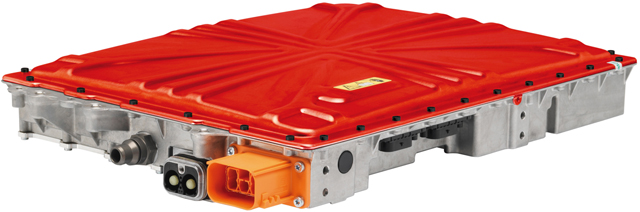
\includegraphics[width = 0.8\textwidth]{figures/brusa_charger.jpg}
	\caption{A svájci BRUSA cég "On-board" töltője} 
	\label{fig:brusa}
\end{figure}

\paragraph{}
Jövőbe tekinthető elképzelés látható \aref{fig:tesla_home} ábrán. A TESLA californiai elektromos autó gyártó cég elképzelése a jövő otthonáról, mely megvalósításához már napjainkban rendelkezésre áll a technológia. Az ábrán egy napelemes cserepekkel burkolt tetejű házat látunk, melynek garázsában található az elektromos autó, illetve a falon a \emph{Powerwall 2.0} nevű akkumulátor csomag, mely az éjszaka folyamán hivatott ellátni a házat elektromossággal. Így tehát megoldódik az otthoni energiaellátás, és a közlekedés problémája is, kevésbé napsütéses időben pedig akár az autó akkumulátora is szolgálhat tartalékként. A falra szerelhető akkumulátor kapacitása egyébként $14\ kWh$, mely egy átlagos háztartást akár 1-2 napig is elláthat elektromos energiával. Hangzatos elképzelés valóban, de a hálózatról való leszakadásra bizonyosan nem alkalmas, hiszen ha sokáig nem tud megfelelő mennyiségű energiát előállítani a rendszer, kénytelenek leszünk a közüzemű elektromos hálózat által biztosított energiára támaszkodni.

\begin{figure}[h]
	\centering
	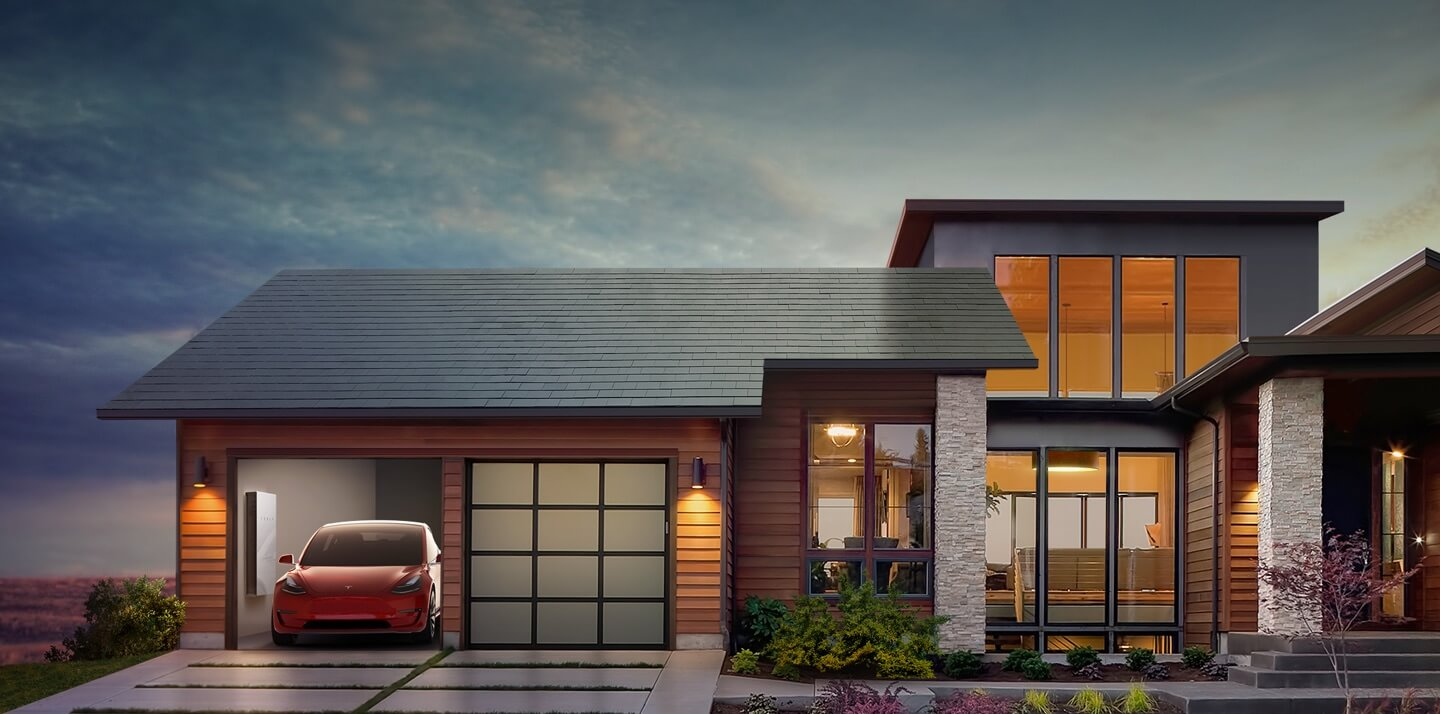
\includegraphics[width = \textwidth]{figures/section-solar.jpg}
	\caption{A TESLA cég elképzelése az integrált otthonról} 
	\label{fig:tesla_home}
\end{figure}



\paragraph{}
A következő probléma az akkumulátorban tárolt energia felhasználása a jármű hajtására. Ehhez nyilvánvalóan szükség van egy motorra, amely többnyire három fázisú szinkrongép. A fenti elvárások most is adottak, hiszen a ezt az eszközt is folyamatosan magunkkal kell vinni. Az integráció, illetve az egyre nagyobb teljesítmény-sűrűség elérésének igényét mutatja, hogy ma már több olyan megoldás is létezik, mely egybe integrálja a motort és annak a meghajtó elektronikáját (ami gyakorlatilag egy három fázisú inverter). \Aref{fig:protean}. ábrán látható az angol \emph{PROTEAN} cég kerékagy motorja, mely a fent leírt rendszert valósítja meg. Biztosítani kell számára a DC nagyfeszültséget, a 12 V-os segéd üzemű táplálást, valamit CAN buszon a vezérlést. Ez a csomag jelentősen megkönnyíti a járműfejlesztő mérnökök dolgát, hiszen nem kell az autóban még egy dobozt elhelyezniük, menet közben pedig egyszerűen csak nyomaték-alapjelet kell a motoroknak küldeni.

\begin{figure}[h]
	\centering
	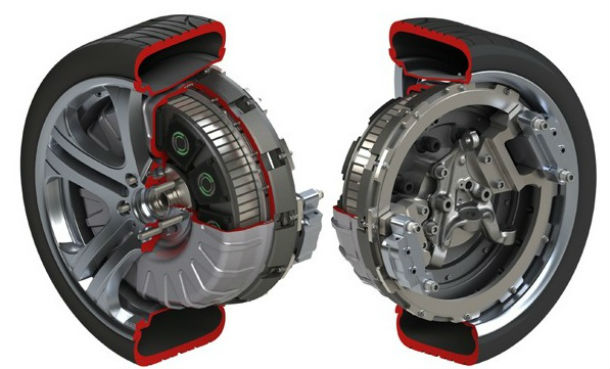
\includegraphics[width = 0.8\textwidth]{figures/protean_motor.jpg}
	\caption{A PROTEAN kerékagymotorja} 
	\label{fig:protean}
\end{figure}

\paragraph{}
Fenti -- és még sok más egyéb -- húzó ágazatok miatt egyre inkább gyorsul a teljesítmény-átalakító eszközök fejlődése, ennélfogva, hogy piacképes terméket lehessen előállítani a fejlesztési időknek is egyre gyorsulnia kell. Ezt támogató eszköz a \emph{Hardware in the Loop} szimulátor. 


\begin{figure}[H]
	\centering
	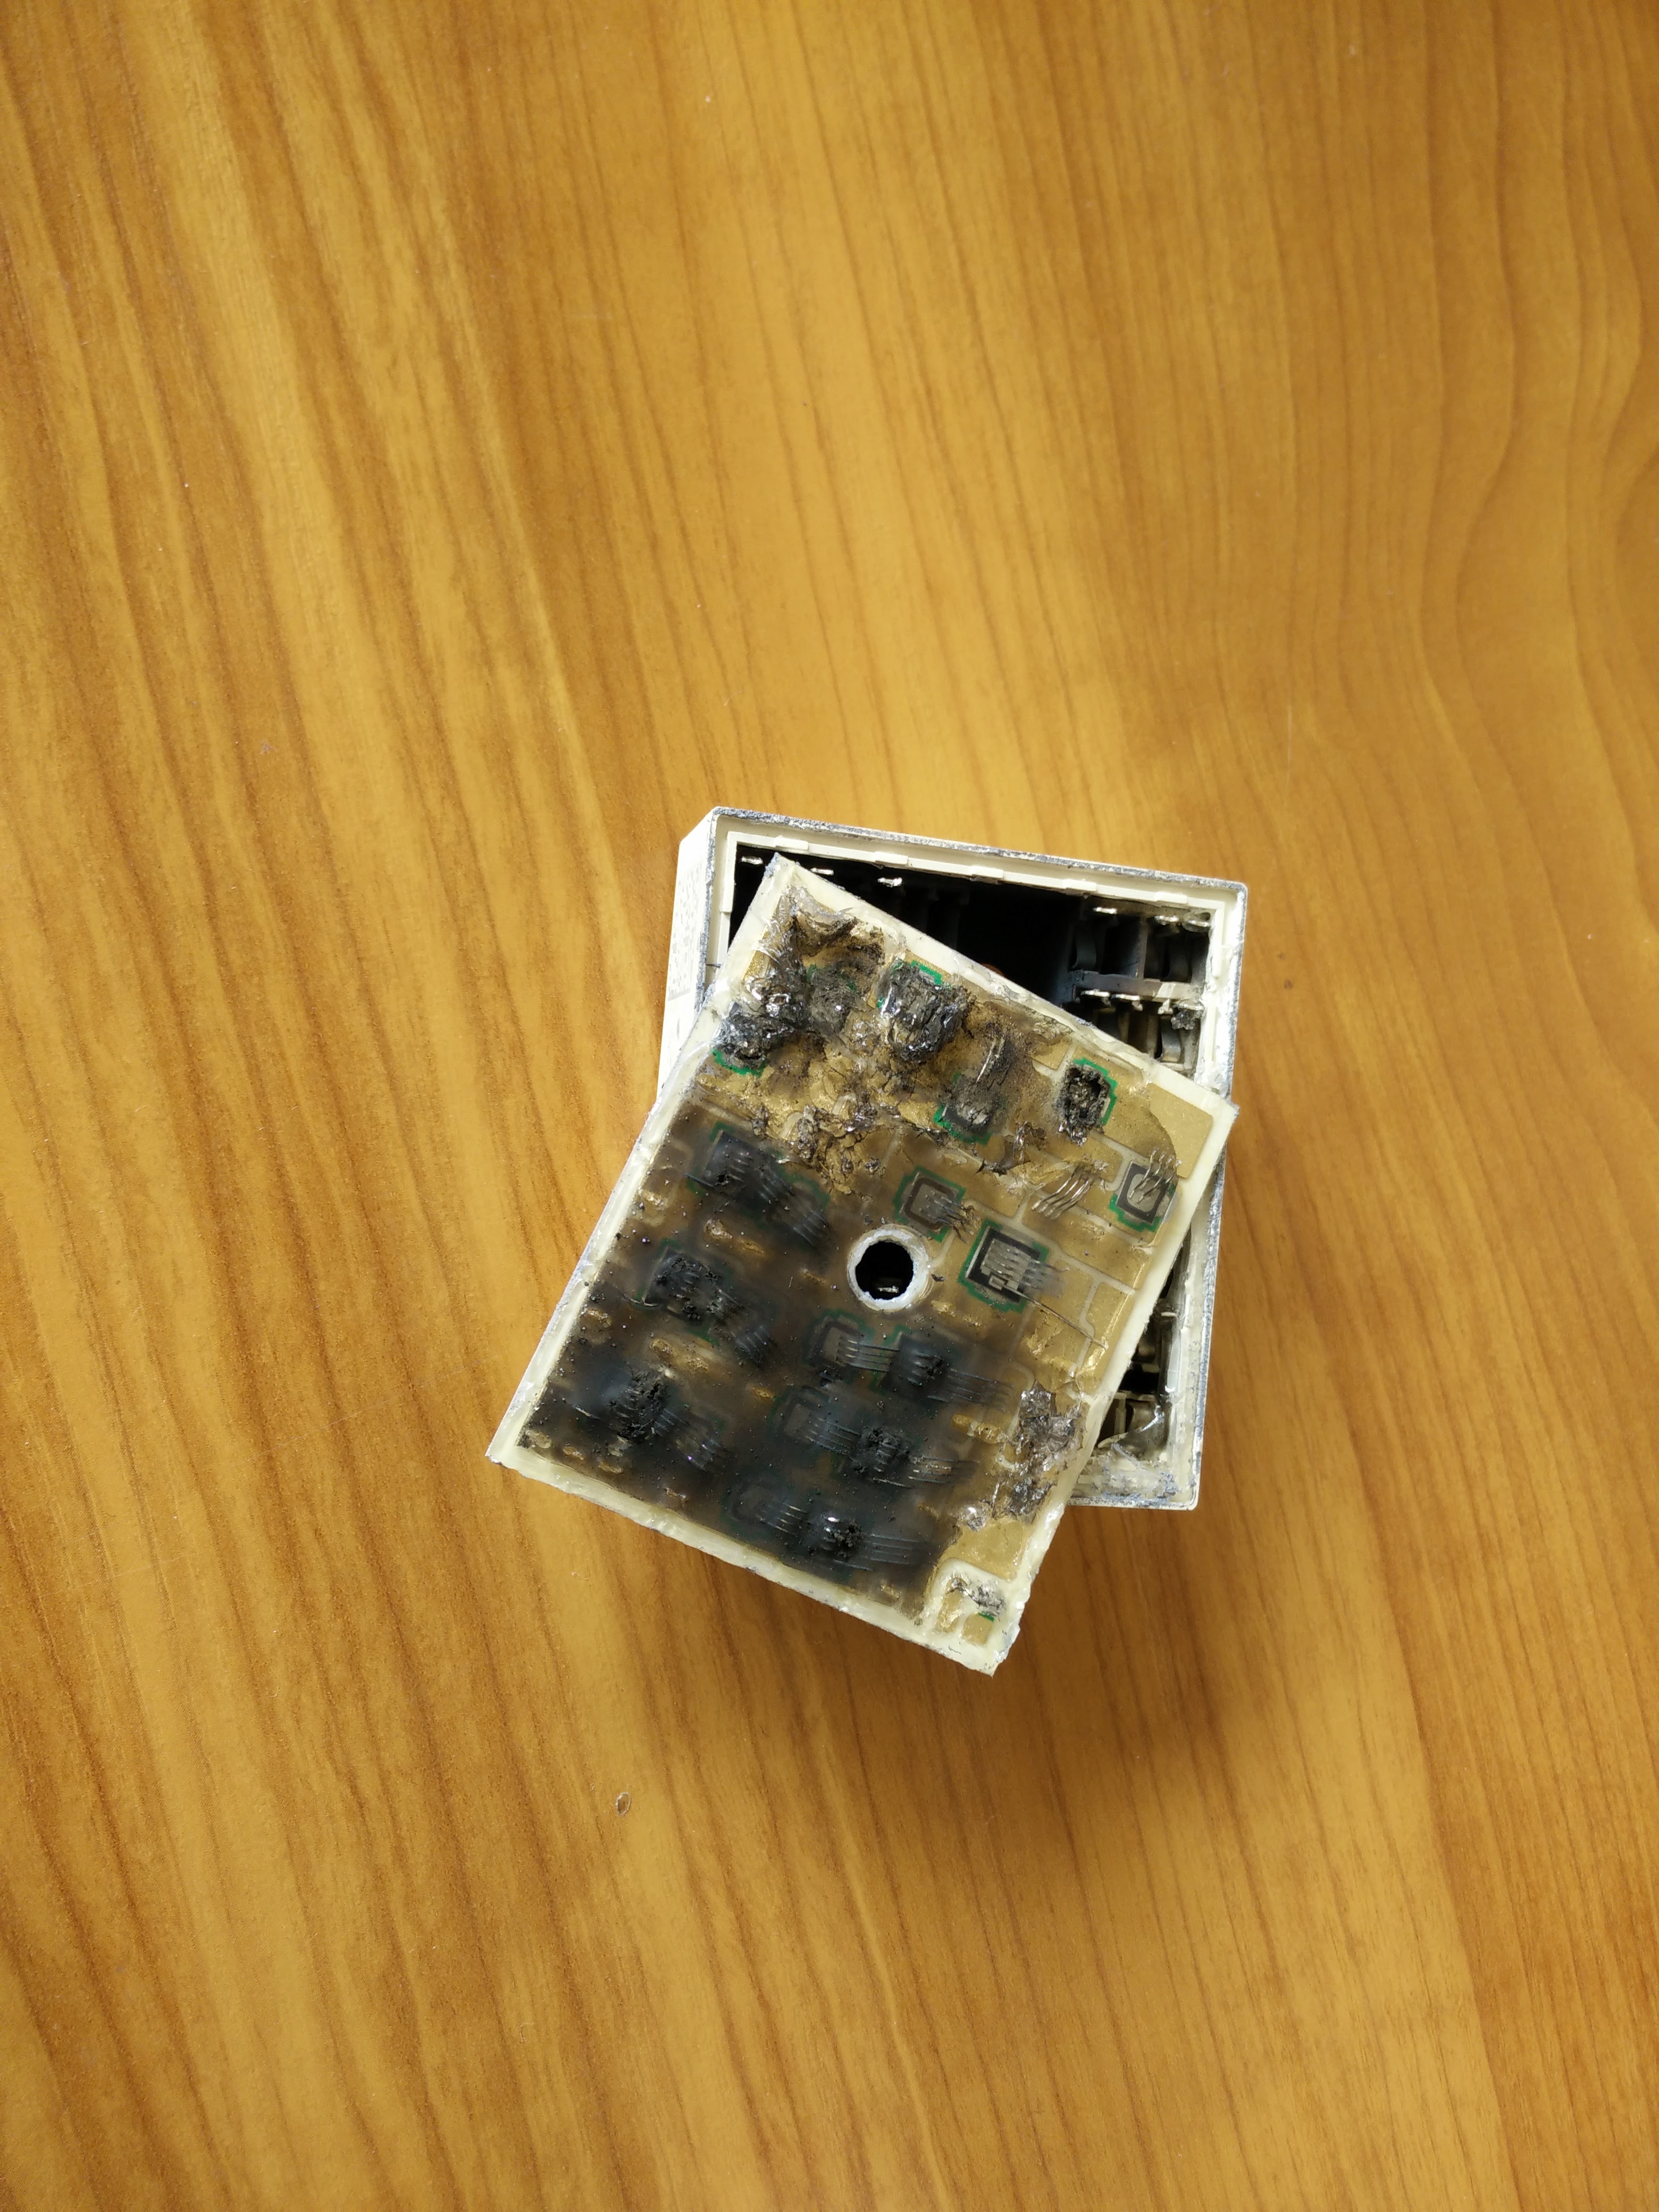
\includegraphics[scale = 0.1]{figures/IMG_20160415_134241.jpg}
	\caption{Felrobbant IGBT modul} 
	\label{fig:blown}
\end{figure}

\paragraph{}
Dolgozatomban végigkísérem egy frekvenciaváltó fejlesztésének folyamatát, különös tekintettel a HIL szimulációra. Megvizsgálom, milyen folyamatok során válik szükségessé, illetve milyen szerepet tölt be az eszköz mind a feljelsztés, mind pedig a tesztelés szakaszában. Maga a teljesítmény átalakító tervezése és vezérlése is igen bonyolult feladat, ezt egy ipari eszközbe kell becsomagolni, melynek kellően robosztusnak kell lennie, hogy az ennek megfelelő szabványoknak és követelményeknek is megfeleljen. Ezért a kifejtés során igyekszem kitekinteni a fejlesztő csapat sokrétűségére is rugalmasságára is, mely ezt segít megvalósítani.
%%----------------------------------------------------------------------------
\chapter*{Zynq SoC}\addcontentsline{toc}{chapter}{Zynq SoC}
%----------------------------------------------------------------------------

\begin{figure}[!ht]
	\centering
	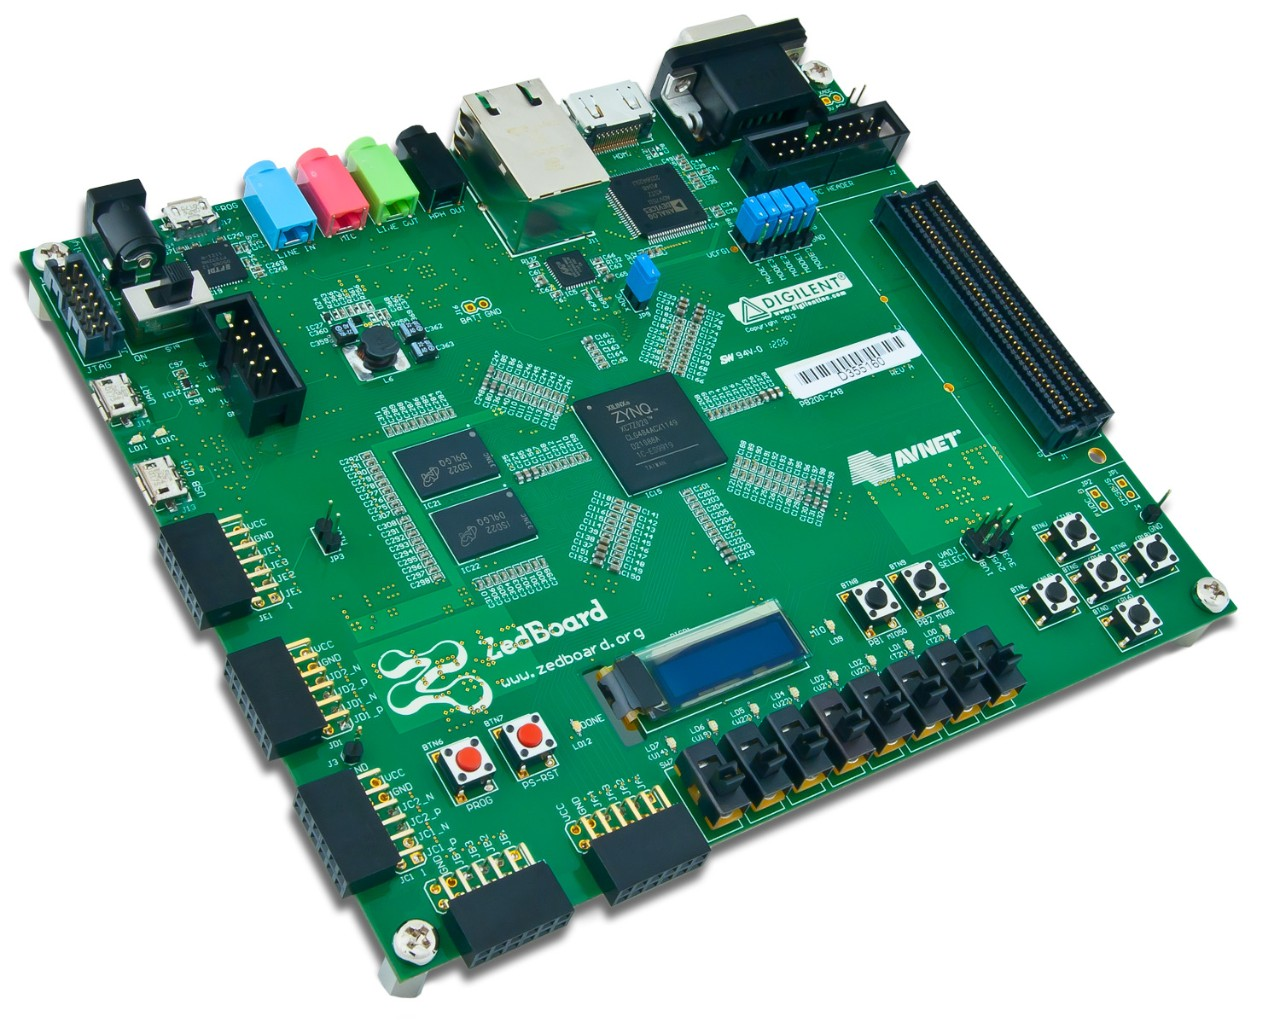
\includegraphics[width = \textwidth]{figures/1381869368208.jpg}
	\caption{A munka során használt ZedBoard} 
	\label{fig:zedboard}
\end{figure}

\begin{figure}[!ht]
	\centering
	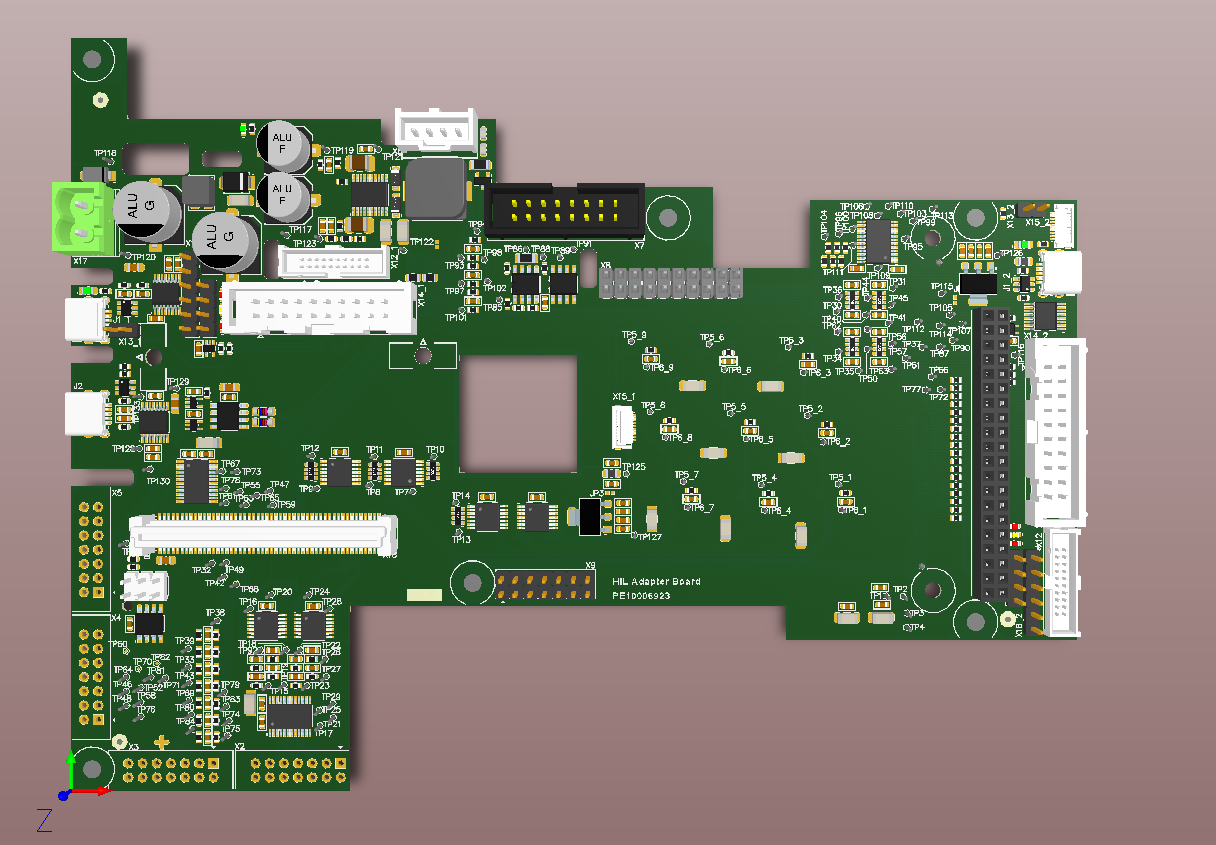
\includegraphics[width = \textwidth]{figures/kieg_nyak.png}
	\caption{A Hyundai által fejelsztett kiegészítő elektornika} 
	\label{fig:kiegnyak}
\end{figure}

\begin{figure}[!ht]
	\centering
	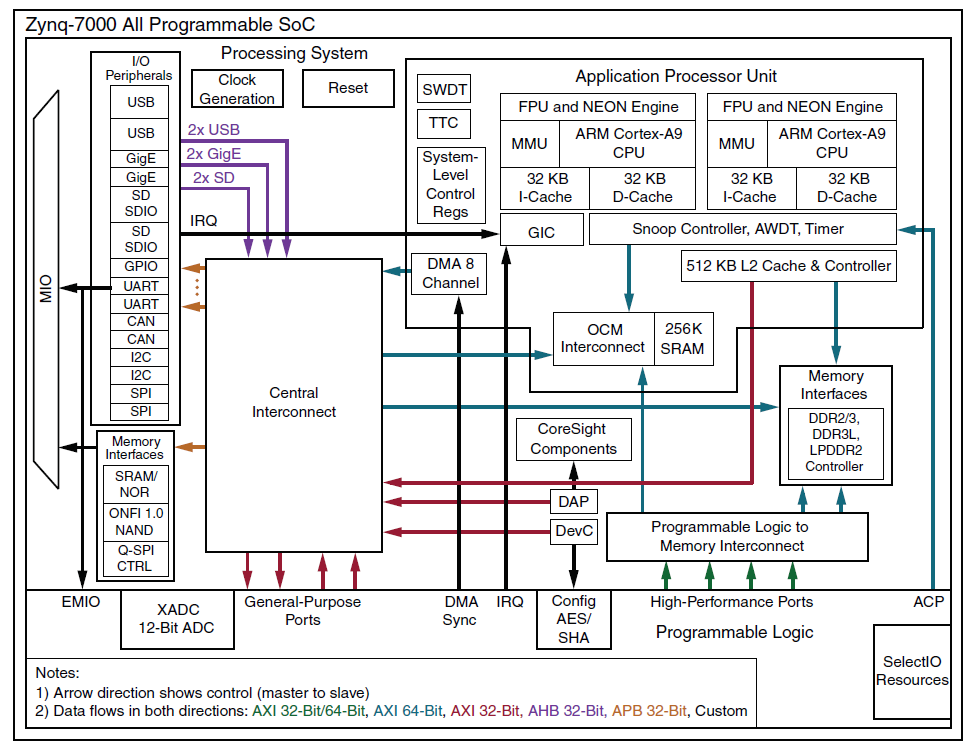
\includegraphics[width = \textwidth]{figures/socfelepites.png}
	\caption{A Xilinx Zynq Z-7000 SoC felépítése\cite{ZynqSOC}} 
	\label{fig:z7000}
\end{figure}
%%----------------------------------------------------------------------------
\chapter*{Az első lépések}\addcontentsline{toc}{chapter}{Az első lépések}
%----------------------------------------------------------------------------

\section{A környezet megismerése}

Ahhoz, hogy a fejelsztést meg tudjuk kezdeni szükségünk van néhány szoftverre, illetve a ZedBoard és a számítógép közötti megfelelő kapcsolat kialakítására. Az egyik legfontosabb szoftver a MATLAB és a Simulink. A MATLAB telepítése után fel kell telepítenünk a ZedBoard-hoz tartozó Hardvare Software Package-et. A telepítés folyamán a ZedBoardhoz tartozó SD kártyára egy speciális image-et is fel kell telepítenünk, ez automatikusan megtörténik. Miután készen vagyunk, csatlakoztatnunk kell a ZedBoard-ot a számítógépünkhöz. Ehhez szükség van egy Ethernet kábelre, illet kettő USB-kábelte, melyek a soros kommunikációt, illetve a JTAG kapcsolatot. A soros portra a kezdeti kapcsoalt miatt van szükség, a JTAG-re az FPGA megfelelő konfigurálásának érdekében, az Ethernetre pedig a szimuláció alatti gyors adatcsere miatt. 

\begin{figure}[!ht]
	\centering
	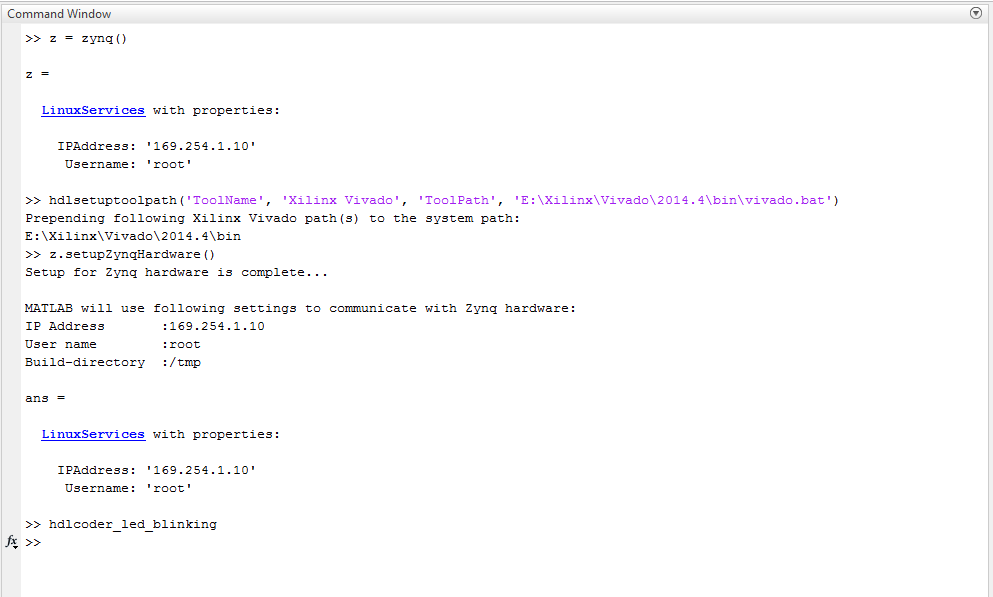
\includegraphics[width = \textwidth]{figures/matlab_1_setup.png}
	\caption{A MATLAB környezet konfigurálása} 
	\label{fig:matlabconf}
\end{figure}

Az alapvető működést egy egyszerű számláló segítségével mutatja be a dolgozat. Ennek modelljét \aref{fig:counter}, illetve \aref{fig:counter_sub} ábárn láthatjuk. \Aref{fig:counter} ábrán a bal oldalon találhatóak a felhasználó bemenetek, a jobb oldalon pedig két \emph{scope}, melyek segítségével megfigyelhetjük a kivezetett változókat, többke között pl. a számláló értékét. \Aref{fig:counter_sub} ábrán pedig a modell belső felépítése látható.

\begin{figure}[!ht]
	\centering
	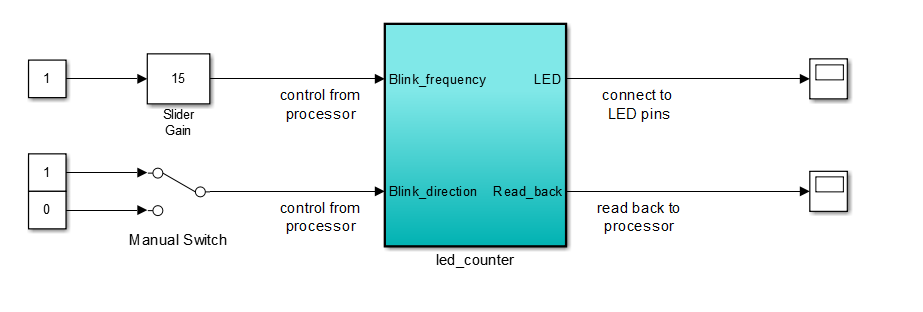
\includegraphics[width = \textwidth]{figures/simulink_1.png}
	\caption{A Simulinkben példa modell} 
	\label{fig:counter}
\end{figure}

Amennyiben a modellel elkészültünk, PC-n futtatva tesztelhetjük a megfelelő működést. Amenyiben elkészültünk, a HDL Workflow Advisor segítségével megkezdhetjük az FPGA projekt létrehozását. Fenti segédprogram végigkísér minket a szükséges lépéseken. Először meg kell adnunk, hogy milyen programmal, mit, és milyen eszközre akarunk készíteni. Jelen esetben a ZedBoard-ra akarunk készíteni egy IP Core-t, a Vivado programcsomaggal.

\begin{figure}[!ht]
	\centering
	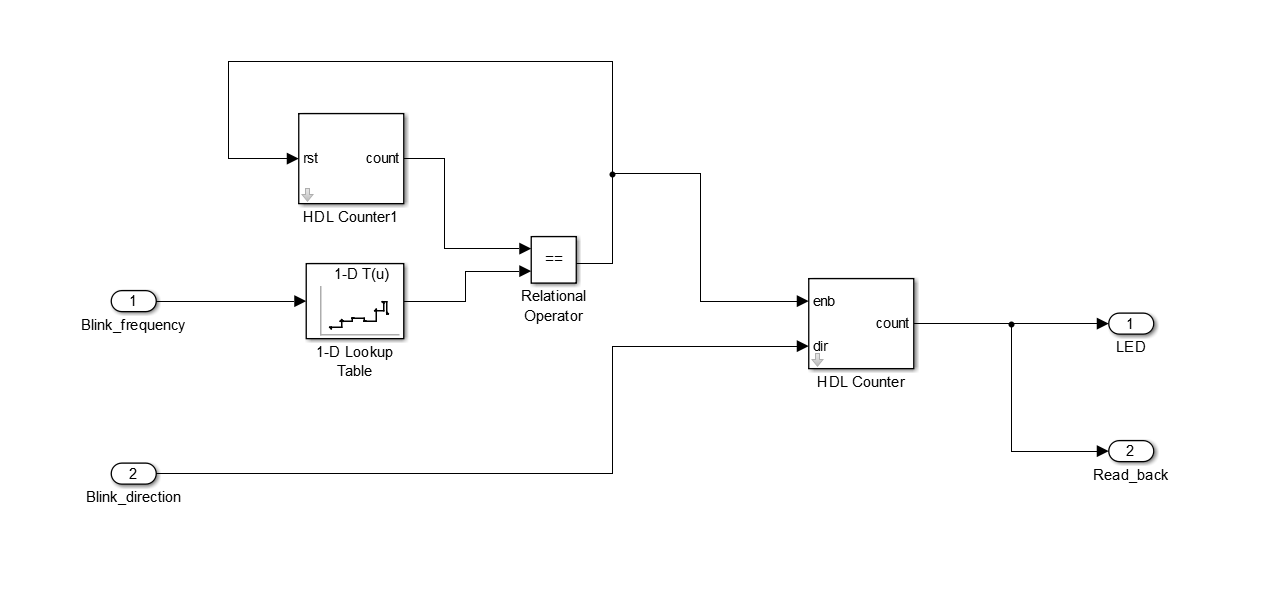
\includegraphics[width = \textwidth]{figures/counter.png}
	\caption{A Simulinkben megvalósított számláló} 
	\label{fig:counter_sub}
\end{figure}

A következő lépésben meg kell adni azt, hogy a fenti kapcsolatok hogyan fognak leképeződni az FPGA-ban fizikailag. A bementeinket egy \emph{AXI4-Lite} buszon keresztül fogjuk elérni. Ez egy kiválasztott címet jelent az SoC közös memóriájában, amire mi tudunk írni, illetve az FPGA blokk onnan olvassa be ezeket az adatokat. Az egyeteln dolog, amit nem így állítunk be, a a számláló, melynek értékét a panelen található LED-ekre is kivezetjük.

\begin{figure}[!ht]
	\centering
	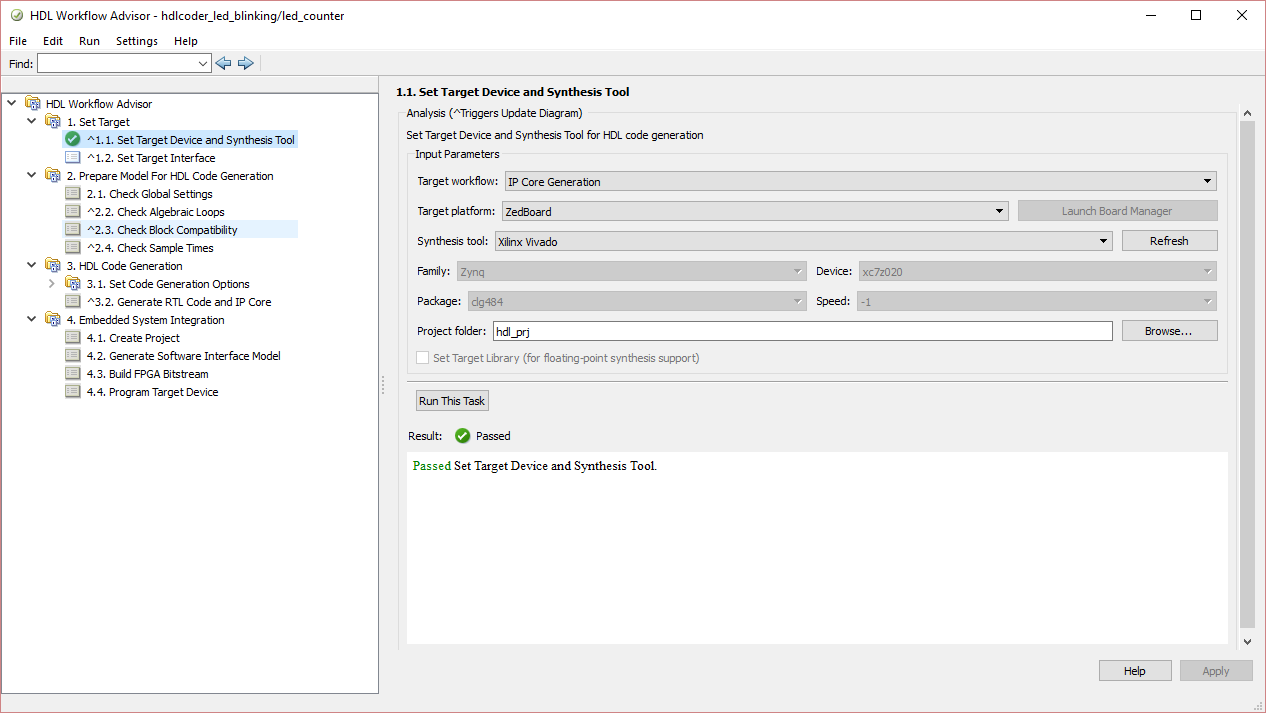
\includegraphics[width = \textwidth]{figures/hdlworkflow.PNG}
	\caption{A HDL kódgenerálás első lépése} 
	\label{fig:hdlgen}
\end{figure}


\begin{figure}[!ht]
	\centering
	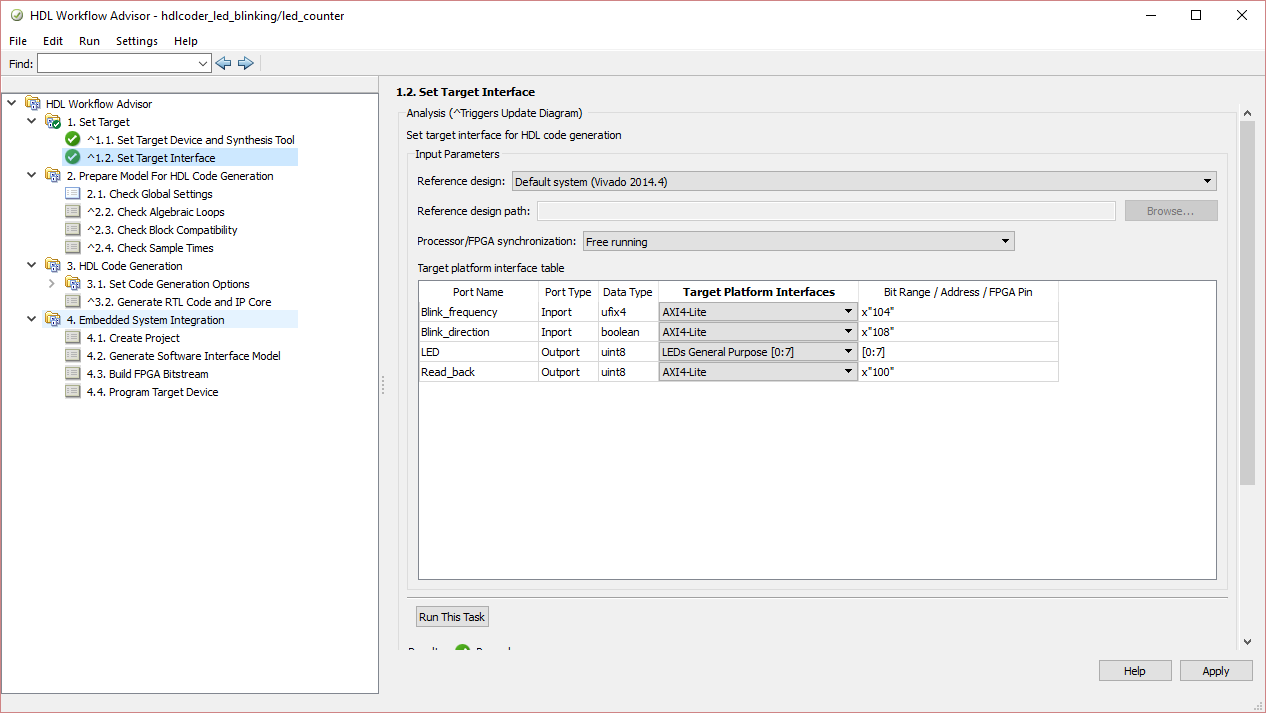
\includegraphics[width = \textwidth]{figures/hdl_2.PNG}
	\caption{A modell elemei és a valós perifériák összerendelése} 
	\label{fig:hdlgen_2}
\end{figure}

Miután ezzel kész vagyunk, a többi lépés gyakorlatilag teljesen automatikus, ezért lefuttathatjuk egyben. Elkészül a Vivado projekt, melynek lefordítására a MATLAB meghívja a Vivado környezetét, elkészíti a bitstreamet, illetve egy C compiler segítségével a modellből készít egy ún. Software Interface modellt. Később ennek segítségével tudjuk a elérni az FPGA-t


\begin{figure}[!ht]
	\centering
	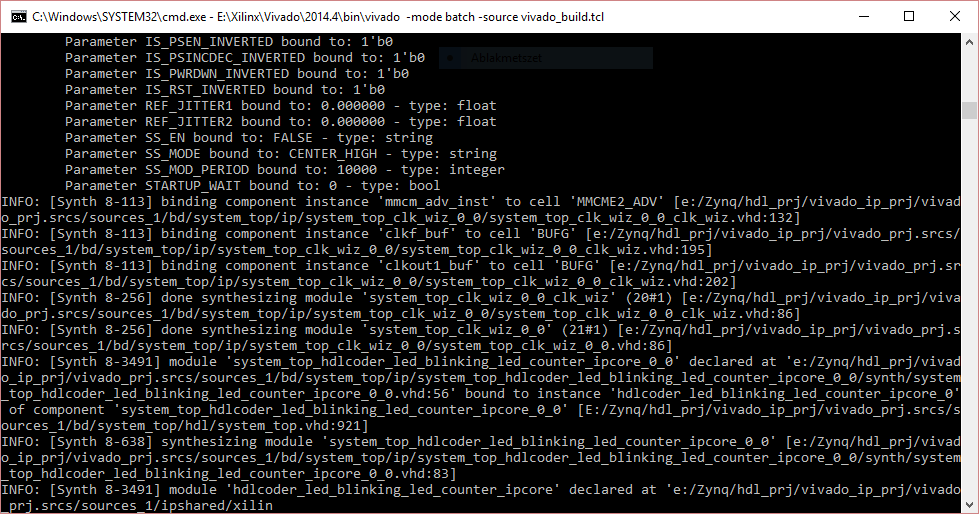
\includegraphics[width = \textwidth]{figures/bitstream.PNG}
	\caption{A HDL projekt fordításásnak kimenete} 
	\label{fig:bitstream}
\end{figure}

\begin{figure}[!ht]
	\centering
	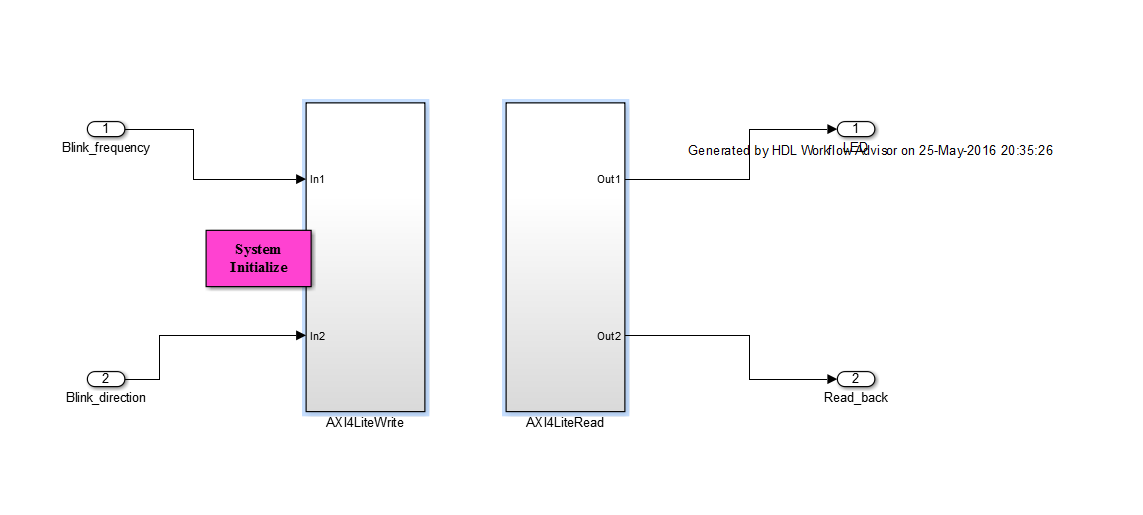
\includegraphics[width = \textwidth]{figures/interface.PNG}
	\caption{A generált Software interface modell} 
	\label{fig:swinterface}
\end{figure}

A Softvare Interface modell első ránézésre ugyan az a modell, mint amit mi készítettünk a folyamat elején. A különbség a színfalak mögött van, ha belenézünk a középső kék blokkba, akkor láthatjuk, hogy itt már nem a számláló van, hanem egy \emph{AXI4LiteWrite} és egy \emph{AXI4LiteRead} blokk található. Tehát a korábbi bemeneteink tényleg leredukálódtak memóriacímekre való írásra, és onnan való olvasásra.

Ahhoz, hogy az FPGA-van valóban kommunikálni tudjunk, ennek a modellnek a futásidejét állítsuk végtelenre, és indísuk el \emph{External} módban. Ez után tudjuk állítani a számlálási frekvenciát, irányt, illetve a kiementeket megnyitva láthatjuk a számláló által létrehozott fűrészjelet is.

\begin{figure}[!ht]
	\centering
	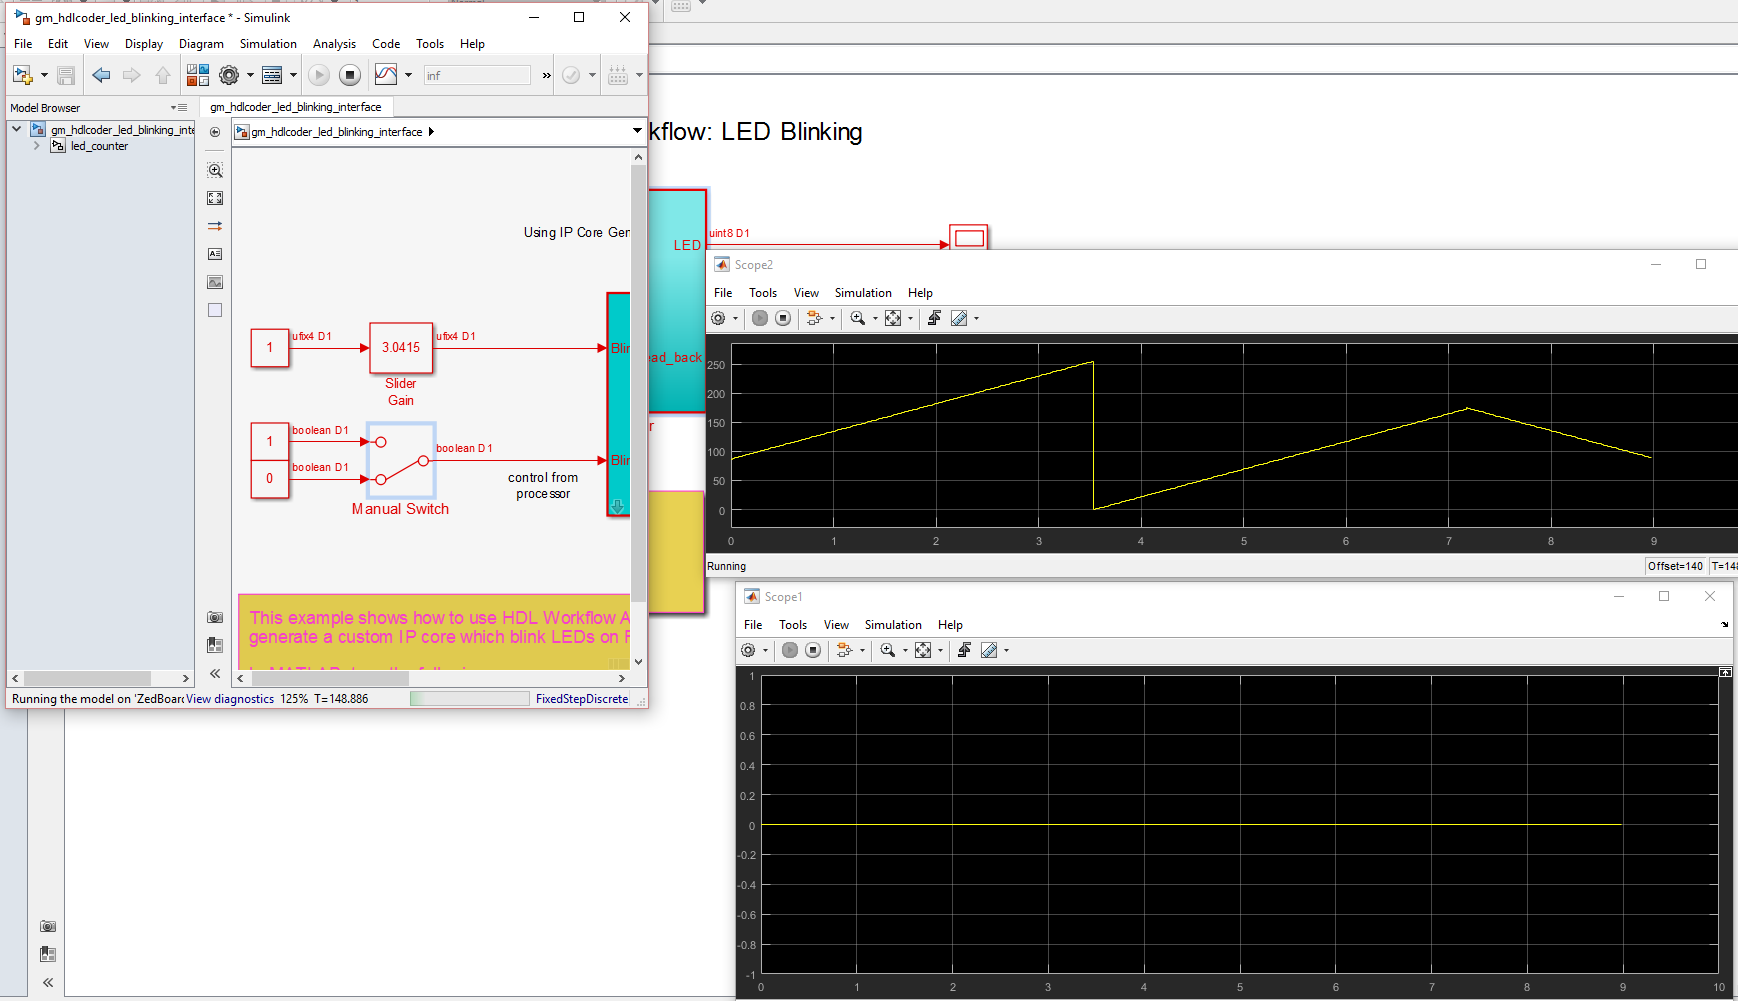
\includegraphics[width = \textwidth]{figures/running.PNG}
	\caption{A futó szimuláció} 
	\label{fig:simualtion}
\end{figure}

%----------------------------------------------------------------------------
\chapter*{Hyundai Technologies Center Hungary Kft.}\addcontentsline{toc}{chapter}{Hyundai Technologies Center Hungary Kft.}
%----------------------------------------------------------------------------

\paragraph{}
A Hyundai Technologies Center Hungary a Hyundai Heavy Industries-nek egy magyarországi fejlesztő központja. A cég 18 éve képviselteti magát a magyar műszaki életben. Bár a névről az első gondolat az autógyártó lehet, azonban a Hyundai egy ennél sokkal nagyobb cég, az autógyár csak egy szelete. A H-TEC a Hyundai Heavy Industries-nek a leányvállalata. A mi cégünk így a HHI-tól kapja a kutatás-fejlesztési megrendeléseket, szorosan együttműködve a dél-koreai kollégákkal.

\begin{figure}[H]
	\centering
	
\includegraphics[width = \textwidth]{figures/hyundai_logo.jpg}
	\caption{A PROTEAN kerékagymotorja} 
	\label{fig:protean}
\end{figure}

\paragraph{}
Az itthoni tevékenysége a cégnek 4 nagyobb csoporra osztható. Ez a beosztás a következőképpen alakul:


\begin{itemize}
	\item{GIS - Gas Insulated Switchgear}
	\item{RM - Rotary Machines}
	\item{TM - Trasformer Machines}
	\item{PE - Power Electronics}
\end{itemize}


\paragraph{}
A részleg, melyben dolgozom a \emph{Power Electronics}\footnote{PE Team} a teljesítményelekotrnikai fejlesztő csoport, a dolgozat írásánk idején ünnepli tizedik évfordulóját haznánkban. A csapatban körülbelül husznöten dolgoznak, az munka az alábbi csoportok között oszlik meg:

\begin{itemize}
	\item{Power Conversion}
	\item{Motor Control}
	\item{Master Control}
	\item{Embedded Control}
	\item{Mechanical}
	\item{Laboratory} 
\end{itemize}

Szerencsére kipróbálhattam magam sok csoportban, foglalkoztam szoftver teszttel, vezélrő algoritmusokkal, illetve a beágyazott szoftverrendszer fejlesztésével is. 




\chapter{Egy frekvenciaváltó tervezése}

\paragraph{}

Tesla 1888-ban bemutatott három fázisú indukciós motorjával, nyilvánvalóvá vált, hogy az ilyen típusú gépek megbízhatóbbak és gazdaságosabbak tudnak lenni, mint az egyenáramú motorok. Jelentős hátrányuk azonban, hogy a vezérlésükhöz háromfázisú feszültséget kell előállítani, mely akkoriban cska egy szintén háromfázisú generátor segítségével volt megoldható. Manapság a háromfázisú teljesítmény a villamos hálózatnak köszönhetően rendelkezésre áll, azonban még így is vet fel prooblémákat ezen motorok üzemeltetése.

A frekvenciaváltó egy olyan eszköz mely váltakozó áramú bemenetből váltakozó áramú kimenetet állít elő, mint ahogy a neve is mutatja, más frekvenciával vagy akár feszültséggel, mint a bemenet. Erre azért van szükség, mert a meghajtani kívánt folyamatnak nagyon valószínű, hogy más igényei vannak, mint amit a hálózat önmagában képes biztosítani. Értem ez alatt azt, hogy közvetlen összeköttetés esetén a motorunk $50\ Hz-el$, vagy ennek egész számú hányadosával tudna forogni, illetve ennek a paraméter a befolyásolása fizikailag csak a motor módosításával lehetséges. Természetesen mint az ipar és az élet minden szegmensében itt is célunk a feladat minél hatékonyabb végrehajtása. A világon a teljes villamosenergia felhasználás mint egy $25\ \%-$-át adják a villamos hajtások és ez a szám folyamatosan nő (pl. az elektromos közlekedés térnyerésével). Az igény tehát nyilvánvaló ezeknek az eszközöknek a folyamatos fejlesztésére.

\begin{figure}[!h]
	\centering
	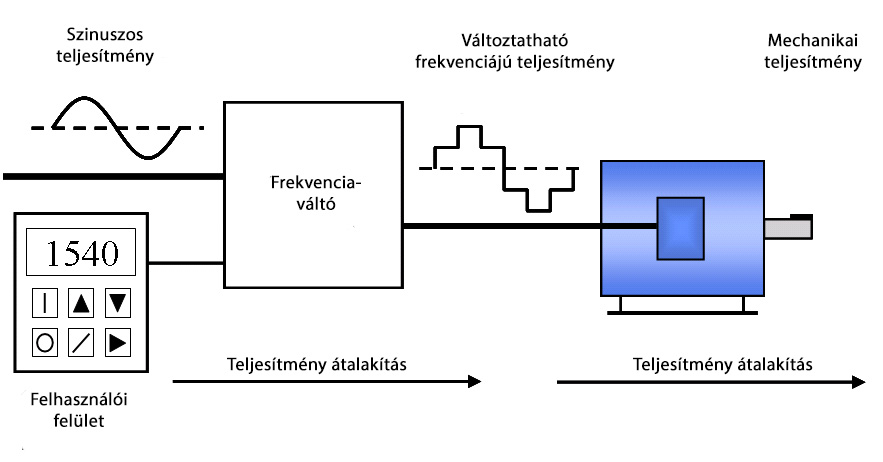
\includegraphics[width = 0.8\textwidth]{figures/VFD_System.jpg}
	\caption{A frekvenciaváltó szerepe} 
	\label{fig:vfd_system}
\end{figure}

Az eszköz feladatát jól összefoglalja \aref{fig:vfd_system} ábra. A hálózatból érkező teljesítményt, a felhasználó által megadott paraméterekkel átalakítjuk, majd a terhelő gépet meghajtuk vele. A modern hajtások ennél jóval szofisztikáltabb működésre is képesek, gondoljunk itt akár távfelügyeletre, identifikációra, vagy esetleg akár vezeték nélküli hozzáférésre.

\paragraph{}
A korábban az ilyen teljesítmény átalakítási feladatokat elektromechanikus berendezésekkel oldották meg, nevezetesen egy motor és generátor párral, ahol is a megfelelő póluspár arány kiválasztásával a frekvenciát módosítani lehetett. Amennyiben szükséges volt feszültségmódosítás is, megfelelő áttételű transzformátor segítségével valósították meg. Ennek a megoldásnak hátránya a nagy teljesítmény esetén nagy méretű villamos gép, ennek megfelelően a kicsi teljesítménysűrűség. A megbízhatóságot csökkenti a mozgó alaktrészek jelenléte és folyamatos igénybevétele, illetve a nagy forgó tömeg is hordoz magában veszélyeket. Ezt követően megjelentek a vákumcsöves eszközök, azonban az igazi áttörést a teljesítményelektronikai félvezető elemek megjelenése okozta.

Ezek a modern eszközök már tartalmaznak mozgó alakrészt (feltéve persze, hogy a reléket és kontaktorokat nem számmítjuk). A félvezető technológia fejlődésével egyre nagyobb és nagyobb teljesítménysűrűségeket tudunk elérni.

\begin{figure}[!h]
	\centering
	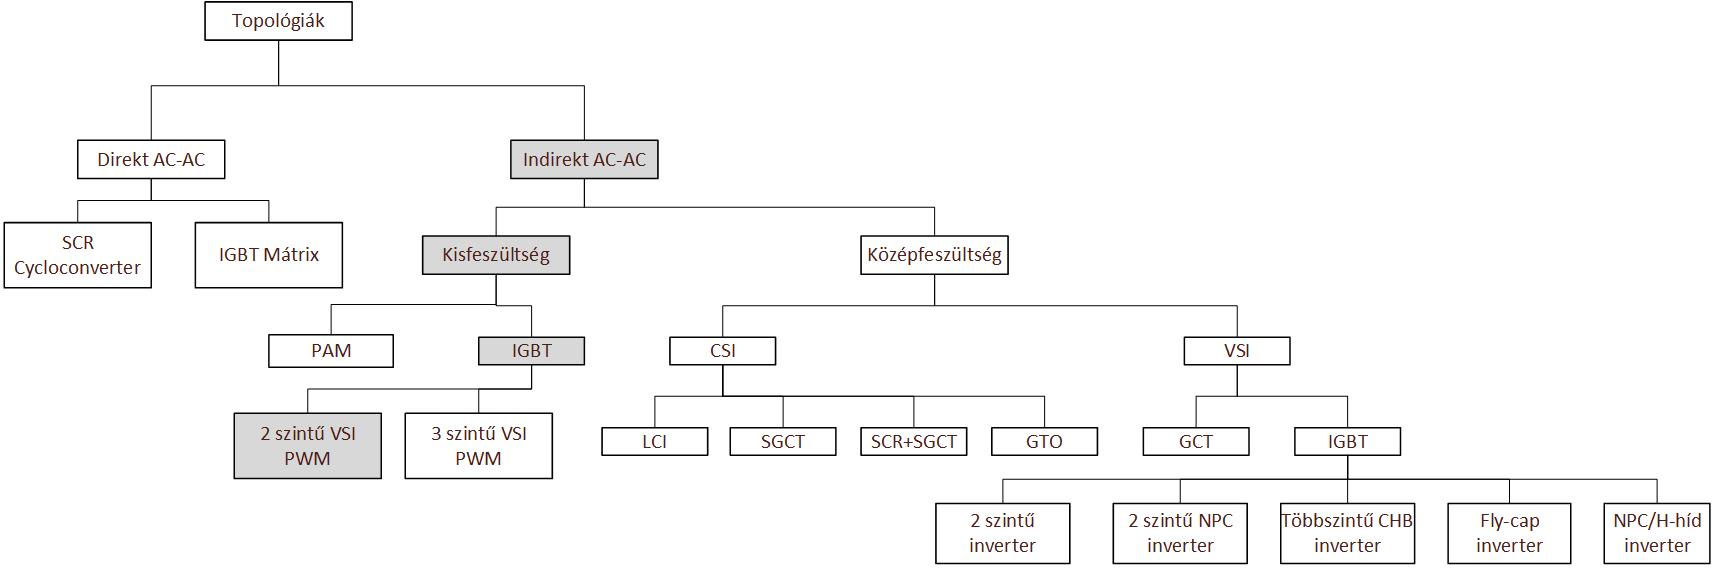
\includegraphics[width = \textwidth]{figures/topologies.jpg}
	\caption{A frekvenciaváltó szerepe} 
	\label{fig:topologies}
\end{figure}

\Aref{fig:topologies} ábrán láthatjuk a napjainkban elterjedt inverter típusokat. Az ábrában szürkével kiemeltem a Hyundai által fejlesztett típust.

\section{Termék specifikáció}

A Hyundai által jelenleg fejlesztett frekvenciaváltó család kis feszültségű, általános célú PWM vezérlet IGBT kapcsolóelemű 2 szintű inverteres frekvenciaváltó, passzív front-end-el, azaz a hálózatra nem tud visszatáplálni. \Aref{fig:family} táblázatban látható a jelenleg fejlesztett termékcsalád.

\begin{table}[]
\centering
\begin{tabular}{|c|c|c|c|l}
\cline{1-4}
\textbf{Név} & \textbf{Teljesítmény (kW)} & \textbf{Áram (A)} & \textbf{Tömeg (kg)} &  \\ \cline{1-4}
\multirow{4}{*}{\textbf{FR1}} & 0,55 & 3,7 & \multirow{4}{*}{6} &  \\ \cline{2-3}
 & 0,75 & 4,8 &  &  \\ \cline{2-3}
 & 1,1 & 6,6 &  &  \\ \cline{2-3}
 & 1,5 & 8 &  &  \\ \cline{1-4}
\multirow{3}{*}{\textbf{FR2}} & 2,2 & 11 & \multirow{3}{*}{10} &  \\ \cline{2-3}
 & 3,7 & 18 &  &  \\ \cline{2-3}
 & 5,5 & 25 &  &  \\ \cline{1-4}
\multirow{2}{*}{\textbf{FR3}} & 7,5 & 31 & \multirow{2}{*}{20} &  \\ \cline{2-3}
 & 11 & 48 &  &  \\ \cline{1-4}
\multirow{3}{*}{\textbf{FR4}} & 15 & 62 & \multirow{3}{*}{37,5} &  \\ \cline{2-3}
 & 18,5 & 75 &  &  \\ \cline{2-3}
 & 22 & 88 &  &  \\ \cline{1-4}
\multirow{3}{*}{\textbf{FR5}} & 30 & 114 & \multirow{3}{*}{66} &  \\ \cline{2-3}
 & 37 & 140 &  &  \\ \cline{2-3}
 & 45 & 170 &  &  \\ \cline{1-4}
\multirow{2}{*}{\textbf{FR6}} & 55 & 211 & \multirow{2}{*}{108} &  \\ \cline{2-3}
 & 75 & 261 &  &  \\ \cline{1-4}
\end{tabular}
\caption{A fejlesztés alatt álló termékpaletta}
\label{fig:family}
\end{table}

Azt, hogy a termék milyen széles területét lefedi az iparnak, jól jellemzi, hogy az ezt leíró dokmentum 52 különböző tételt különböztet meg. A teljesség igénye nélkül a felvevő piac néhány szelete:

\begin{itemize}
	\item{Nagyfeszültségű légkondícionálók}
	\item{Élelmiszeripar}
	\item{Textilipar}
	\item{Szállítószalagok}
	\item{Csomagolás és cimkézés}
	\item{Nyomtatás}
	\item{Gépi megmunkálás}
	\item{Autóipar}
\end{itemize}

A hardveres funkcionalitás nagyjából megegyezeik minden esetben, az igazán nagy különbség az egyes területek között a szoftver funkcionalitásában van. Egy szállítószalag esetében fontos a pontos fordulatszám tartása, vagy a pontos pozíció beállítása, míg más felhsználás esetében a potos nyomatékszabályozás lehet fontos, ilyen lehet pl. a villamos vontatás.

Amennyiben külön nincsen jelölve, a dolgozat a továbbiakban az FR1 kódjelű, legkisebb frekvenciaváltóra hivatkozik a példák esetében.

\section{Az eszköz felépítése}

\paragraph{}
A frekvenciaváltó egyenirányítja a bejövő hálózati feszültséget, egy köztes energiatárolóban, az ún. \emph{DC-link} kondenzátorban tárol némi energiát, hogy a feszültség lengésést alacsonyan tartsa, majd egy kimeneti inverterrel előállítja a szükséges jelalakot. Ezt a vázlatot láthatjuk \aref{fig:vfd_schema} ábrán, kiemelve a hálózatot modellező ellenállást és induktivitást.

\begin{figure}[h]
	\centering
	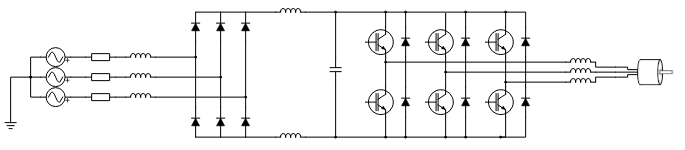
\includegraphics[width = \textwidth]{figures/VFDschematic_choke.png}
	\caption{A frekvenciaváltó egyszerű felépítése} 
	\label{fig:vfd_schema}
\end{figure}

Itt természetesen csak egy vázlatos ábrázolás látató, ezen nem szerepelnek a megható elektronikák, a vezérlés, a mérések, és még sok más. Jól látható azonban, hogy a folyamatra egyedül a félhidak vezérlésével tudunk hatni. A Frame 1-ben a kimeneti IGBT-k és diódák egy tokban vannak, egy Semikron SKiiP 24NAB12T4V1 modulban. \cite{sutozoli} \cite{ctan}

\section{A szükséges kompetenciák}

A felépítés alapján elmondható, hogy egy iylen termék összeállítása nagyon bonyolult feladat, sok területet lefed, sok féle kompetenciára van szükség. A teljesítményelektronikai elemek és kapcsolálos megtervezése gyakorlatilag csak az első gondolat. Ezen túl szükséges még a termikus méretezés, a vezérlő elektronikák tervezése, a különböző mérések megvalósítása. Amikor már ezzel is készen vagyunk, akkor a frekvenciaváltó tervezése elektronikai szempontból késznek mondható. Nem sabad megfeledkezni azonban arról, hogy ez egy készülék, melynek a mechnaikus felépítéséről is gondoskodni kell. Itt kerülnek képbe a konstrukcióval foglalkozó gépész kollégák.

\begin{figure}[h]
	\centering
	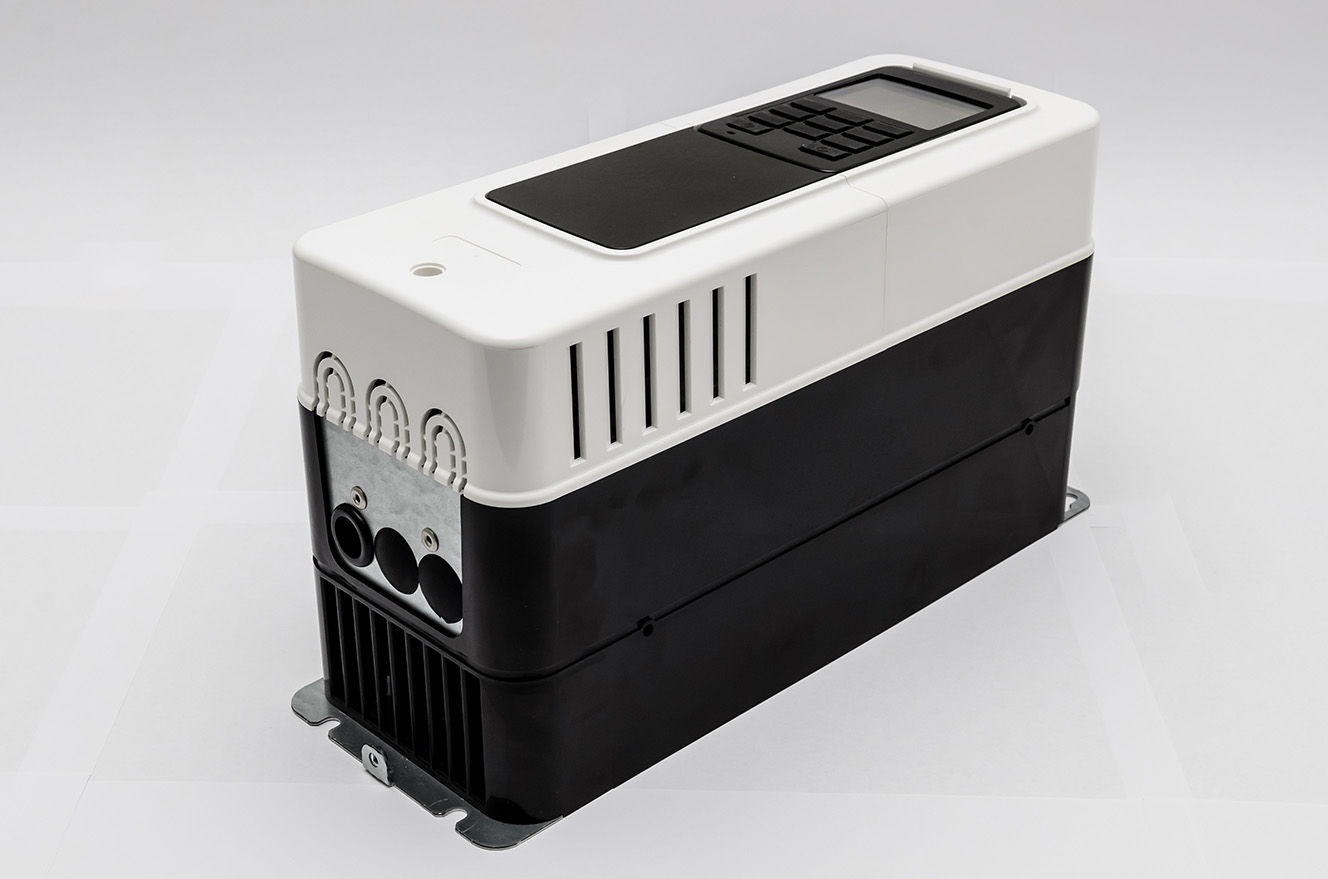
\includegraphics[width = 0.8\textwidth]{figures/n700_proto.jpg}
	\caption{A frekvenciaváltó egyszerű felépítése} 
	\label{fig:n700_proto}
\end{figure}

A feladat már eddig is kellőképpen összett volt, de a termékünk még mindig nem működik. Hiányzik belőlea szoftver, mely önmagában nagyon szerteágazó munka. Először is elő kell állítani a megfelelő szabályzókat, melyek segítsgével elő tudunk állítani színuszos kimenetet, gondoskodni kell a kapcsolóelemek megfelelő modulációjáról. Foglalkozni kell a magasabb szintű funkcionalitás megvalósításával, a különböző kommunikációs vonalak kezelésével, magának a rendszernek a menedzselésével. A HMI\footnote{Human-Machine Interface}-n is meg kell jelenteni információt, biztosíani kell lehetőséget a beavatkozásra. Amennyiben úgy gondolá az olvasó, hogy ez még nem annyira bonyolult, akkor figyelmébe ajánlom a PC-s szoftvert, melyet szintén el kell készíteni, ha egy jól használható terméket kívánunk előálltani. 

\todo[inline]{Félbehagyott gondolat}

\begin{figure}[h]
	\centering
	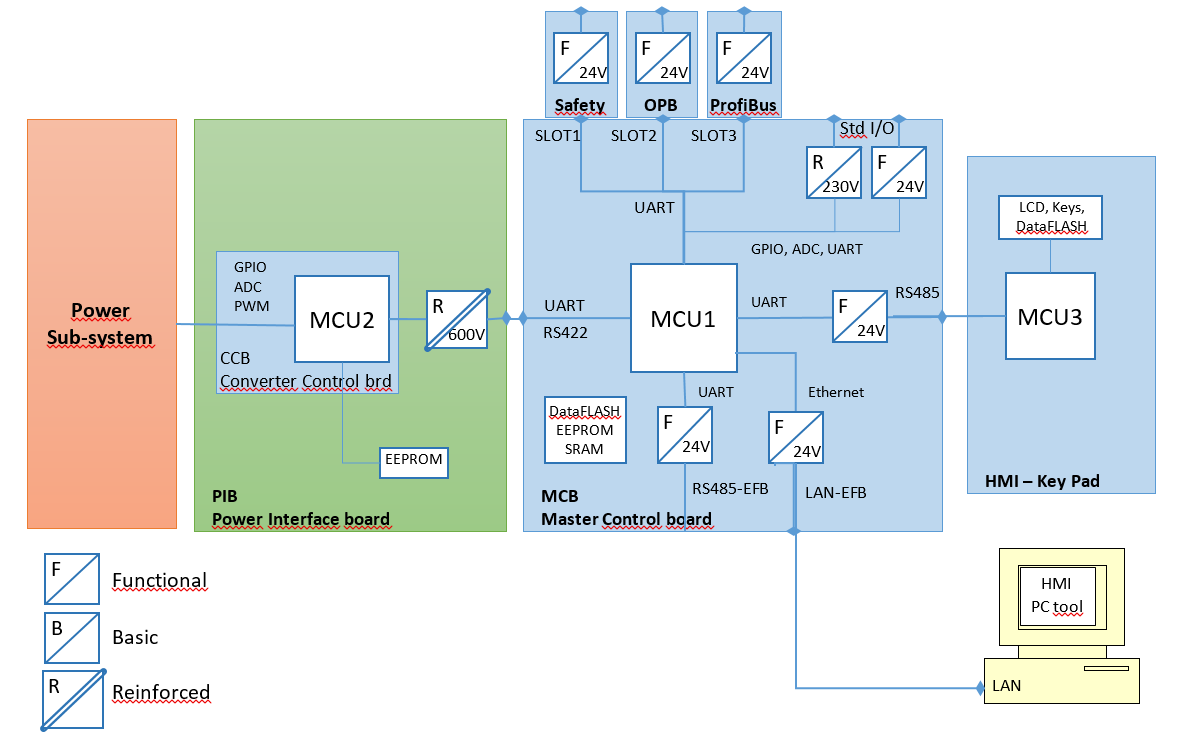
\includegraphics[width = \textwidth]{figures/architect.png}
	\caption{A vezérlő elektronika blokkvázlata} 
	\label{fig:hw_architect}
\end{figure}

\Afigref{hw_architect} ábrán látható a különböző elemek kapcoslata, illetve a kommunikávó közöttük. A CCB feladat a teljesítményátalakítás közvetlen irányítása. Ez a kártya végzi az analóg méréseket, és ezen mérések, illetve a beérkező alapjel alapján előállítja az IGBT-ket vezérlő PWM jeleket. A szoftveres védelmekről is ez a szint gondoskodik. A következő az MCB, mely az egyel magasabb szintű vezérlésért felel. Ez jelenti a kommunikációt más eszközökkel, a különböző terepi buszukon, etherneten, vagy RS-485-ön. Rendelkezik továbbá általános célú digitális és analóg be és kimenetekkel, melyek működése felhasználói igények szerint testre szabható. Ez az eszkösz felelős a számítógépes konfiguráló szoftverrel való kommunikációért, valamint a HMI vezérléséért is. A fejlesztett HIL szimulátor szempontjából ez a három elektronika bír szereppel, ezek közül a HMI csak közvetetten, mivel az MCB-n keresztül kapcsolódik a rendszerhez.

\section{A fejlesztés folyamata}

A teljesítményelektronikai eszközök fejlesztésének a nehézésége abban rejlik, hogy a kisebb teljesítményű modell nem feltéltlenül viselkedik úgy, mint nagyáramú társa. A fenti felíráson az is jól látszik, hogy bizonyos folyamatok párhuzamosíthatóak. A szoftverfejlesztés elkezdődhet a nagyáramú elektornika tervezésésvel együtt, illetve a vezérlő elektronikák is tervezhetően a kezdeti specifiákciók, illetve a a kapcsolódási pontok definiálása után. A fejlődő szoftver teszteléséhez aszonban elengedhetelen, hogy a beágyazott eszköz megkapja a szükséges gerjesztéseket a külvilágtól. Amíg nem áll rendelkezésre a valós eszköz, addig ezt egy szimulátorral vagyunk kénytelenek megvalósítani. Ez a Hardware-in-the-Loop szimulátor. Az eszköz jól jön azonban amikor már a valós frekvenciaváltó is rendelkezésre áll. Az egyes szoftvermódosításokat célszerű kipróbálni ezen az eszközön először, mert egy hiba könnyedén végzetes következményekkel járhat a valós invertren.

\chapter{HIL felépítése}

Nyilvánvaló tehát, hogy napjainkban, a modern teljesítmény elektronikai eszközök fejlesztéséhez elengedhetetlen a HIL szimulátor alkalmazása. Bár az eszköz fejlesztése jelentős terhet ró a készítőkre, segítségével csökkenthető a tervezésre fordítandó idő, a fejlesztési folyamatok párhuzamosításával. Segítségével elkerülhetőek a költséges és veszélyes hibák a fejlesztés alatt, hiszen a teljesítmény elektronikai elemek csak matematikai modell formájában jelennek meg a rendszerben. Ezen felül a tesztelés minősége is jelentősen javítható a költségek csökkentése mellett. Ilyen szimulátorból sok futhat egymás mellett párhuzamosan, a valós elektronika többszöri felépítése nélkül. Így sok különböző teszteset futtatható egyszerre, akár ciklikusan, emberi felügyelet nélkül. \cite{sutozoli}\cite{low_cost_rt_hil}\cite{hw_emu}

\section{Hardware felépítése}

A HIL szimulátor hardware nem más, mint egy interface elektronika a vezérlő hardware-ek és a szimulációt végző FPGA között. \Afigref{hw_architect} ábrán láthatóak a vezérést végző elemek. A HIL szimulátor feladata a bal oldali, Power Subsystem blokkból érkező jelek előállítása, illetve a vezérlő jelek fogadása.

\subsection{CCB és MCB csatlakozó}
\todo[inline]{Meg kell rendesen foglalmani a kis mondandóm}
A szimuláció során a PIB nem szükséges, ezért az MCB és a CCB kapcsolatát is a HIL elektronika biztosítja. A két eszköz között a kommunikáció UART-on valósul meg. A kivitelezés számomra több szempontból is érdekes, mert a sebesség $9\ Mbaud$, illetve a fizikai réteg sem teljesen szokványos. Az UART jelek differenciálisan kerülnek átvitelre az MCB felé, de az Rx és a Tx egy-egy külön érpárt kapott. Az MCB-n keresztül érkeznek még ezen felül a \emph{Sto1X} és a \emph{Sto2X} jelek. Ezek a jelek szintén speciálisak, az eszköz vészleállításáért felnek. A CCB-vel való kommunikáció \aref{table:ccbsignals}. táblázatban felsorolt jelek segítségével valósul meg. 

\begin{table}[]
\centering
\begin{tabular}{|l|l|l|l|}
\hline
\textbf{Név}   & \textbf{I/O} & \textbf{A/D} & \textbf{Leírás}                 \\ \hline
UoutU          & Digital      & Bemenet      & Az U fázis nullátmenetének jele \\ \hline
UoutV          & Digital      & Bemenet      & A V fázis nullátmenetének jele  \\ \hline
UoutW          & Digital      & Bemenet      & A W fázis nullátmenetének jele  \\ \hline
Sto1SatusX     & Digital      & Bemenet      &                                 \\ \hline
Sto2SatusX     & Digital      & Bemenet      &                                 \\ \hline
MCB\_TxD       & Digital      & Kimenet      &                                 \\ \hline
MCB\_RxD       & Digital      & Bemenet      &                                 \\ \hline
EEPROM\_SDA    & Digital      & Be/Kimenet   &                                 \\ \hline
EEPAROM\_SCL   & Digital      & Kimenet      &                                 \\ \hline
RectStatusC    & Digital      & Bemenet      &                                 \\ \hline
PrechargeCtrlX & Digital      &              &                                 \\ \hline
IgbtBFltX      & Digital      &              &                                 \\ \hline
IgbtBRdy       & Digital      &              &                                 \\ \hline
IgbtBRstX      & Digital      &              &                                 \\ \hline
IgbtPsuCtrlX   & Digital      &              &                                 \\ \hline
IgbtInvFltX    & Digital      &              &                                 \\ \hline
IgbtInvRdy     & Digital      &              &                                 \\ \hline
IgbtInvRstX    & Digital      & Kimenet      &                                 \\ \hline
IgbtU1         & Digital      & Kimenet      &                                 \\ \hline
IgbtU2         & Digital      & Kimenet      &                                 \\ \hline
IgbtV1         & Digital      & Kimenet      &                                 \\ \hline
IgbtV2         & Digital      & Kimenet      &                                 \\ \hline
IgbtW1         & Digital      & Kimenet      &                                 \\ \hline
IgbtW2         & Digital      & Kimenet      &                                 \\ \hline
IgbtB          & Digital      & Kimenet      &                                 \\ \hline
FanPsuCtrC     & Digital      & Kimenet      &                                 \\ \hline
FanExtCtrC     & Digital      & Kimenet      &                                 \\ \hline
FanIntCtrC     & Digital      & Kimenet      &                                 \\ \hline
FanExtSpeedC1  & Digital      & Kimenet      &                                 \\ \hline
FanExtSpeedC2  & Digital      & Kimenet      &                                 \\ \hline
5V\_Loopback   & Power        &              &                                 \\ \hline
TIgbtW         & Analog       & Bemenet      &                                 \\ \hline
15VCM          & Analog       & Bemenet      &                                 \\ \hline
TIgbtV         & Analog       & Bemenet      &                                 \\ \hline
UdcMN          & Analog       & Bemenet      &                                 \\ \hline
UdcMP          & Analog       & Bemenet      &                                 \\ \hline
IWN            & Analog       & Bemenet      &                                 \\ \hline
IWP            & Analog       & Bemenet      &                                 \\ \hline
TIgbtU         & Analog       & Bemenet      &                                 \\ \hline
TIgbtB         & Analog       & Bemenet      &                                 \\ \hline
IUP            & Analog       & Bemenet      &                                 \\ \hline
IUN            & Analog       & Bemenet      &                                 \\ \hline
IVP            & Analog       & Bemenet      &                                 \\ \hline
IVN            & Analog       & Bemenet      &                                 \\ \hline
TA             & Analog       & Bemenet      &                                 \\ \hline
5VSto1         & Analog       & Bemenet      &                                 \\ \hline
5VSto2         & Analog       & Bemenet      &                                 \\ \hline
UdcP           & Analog       & Bemenet      &                                 \\ \hline
UdcN           & Analog       & Bemenet      &                                 \\ \hline
\end{tabular}
\caption{A CCB jelei}
\label{ccbsignals}
\end{table}

Ezek azok a jelek, amiket a HIL-nek vagy szimulálnia, vagy pedig fogadnia kell. Kivételt képez ez alól az \emph{5V\_Loopback}. Ennek a funkciója az, hogy létre lehet hozni a PIB-en olyan áramköri részeket, melyek az $5\ V$-os táplálást csak a CCB-n keresztül kapják meg, így nem indulnak el csatlakoztatott kártya nélkül.

A digitális jelek esetében a feladat egyszerű, csak a CCB és az FPGA közti jelszint különbséget kell megoldani. Ebben egy \emph{74LVC8T245PW} típusú level-shifter lesz segítségünkra. A CCB a jelekt $5\ V$-os tartományban adja ki, illetve fogadja, az FPGA maximális kiementi feszültésge $3,3\ V$, és nem is állnak rendelkezésre nagyobb feszültséget toleráló lábak. A kisebb feszültségre való átalakításra lehetséges megoldás a feszültségosztó is, de a nagysebességű jelek dinamikájának megőrzése érdekében inkább itt is a level-shiftert választottam. A lassabb jelek esetében maradtam a feszültségosztóval való megoldásnál.

Analóg jeleket tekintve csak bemenet találhat óa CCB-n. Ezen jelek előállítását Sigma-Delta átalakítók segítségével oldottam meg, melyről részletesebben később lesz szó.

A fent említett jeleken kívül a HIL-en elhelyeésre került az ULINK és az St-Link debuggerek csatlakozója is, a fejlesztés kényelmesebbé tételének érdekében. A CCB-re a JTAG jelei egy külön flat-flex kábel segítségével csatlakoznak. Ennek a mechanikai teherbíása igen alacsony, így pedig nem kell egy külön kártyára csatlakoztatni, kockáztatva ezzel az elmozdulást, kontakthibát vagy vezetékszakadást.

\todo[inline]{Blokkvázlat a HIL-ről}

\subsection{Tápegység}
A kártya $24 V$-os tápfeszültségre lett tervezve. Ebből egy Linear Technologies \emph{LT3845AEFE#PBF} szinkron buck tápegység vezérlő IC és a hozzá tartozó külső apparátus állítja aelő az $5 V$-os tápfeszültséget mind az FPGA mind pedig a CCB számára. A tápegység maximálisan $6 A$ terhelhetőségű, amely előser soknak tűnhet, de az FPGA fogyasztását jelentpsen befolyásolja a benne található firmware, így elképzelhető az kapacitás teljes felhasználása is, kis teljesítmény esetén edig hatékony tud maradni az ún. \emph{Burst mode} működési mód segítségével.

\subsection{ZTEX kártya}

Egy iylen teszt és fejlesztési eszköz fejlesztése során az egyik legfontosabb szempont a modularitás. Nem láthatjuk előre feltétlenül, hogy a későbbiekben mire lesz szükség. Az FPGA önmagában biztosít modularitást, hiszen cserélhető benne a hardware, jelen esetben a megvalósított matematikai modell. Ezen felül egy közel 500 lábbal rendelkező BGA tokos FPGA-hoz a nyáktervezés sem triviális feladat. A megfelelő lábak kivezetéséhez legalább 6-8 rétegre van szükség, és nagyon sok hibalehetőséget tartogat magában. Ezek miatt egy FPGA modul alkalmazása mellett döntöttünk. Bár az elérhető GPIO lábak mennyisége így korlátoztt, az FPGA-t működtető áramkör garantáltan működőképes, illetve a saját tervezésű elektornika bonyolultsága is jelentősen csökken.

\begin{figure}[!ht]
	\centering
	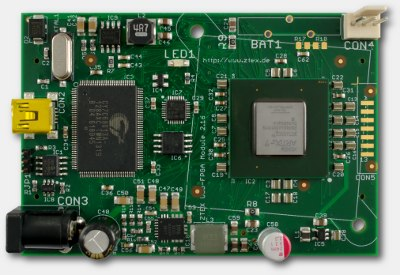
\includegraphics[width = 0.75\textwidth]{figures/fpga216.jpg}
	\caption{A ZTEX 2.16 FPGA board} 
	\label{fig:ztex}
\end{figure}

\Aref{fig:ztex} ábrán látható ZTEX panel mellett tettem le a voksom. A kártyáról kivezetésre kerültek a JTAG interfész jelei is, azonban az ehhez az FPGA-hoz való Xilinx debugger nem áll rendelkezésre. A ZTEX kártyán azonban egy Cypress mikorovezérlő segítségével, \emph{libusb} driver segítségével betölthető a bitstream mind a RAM-ba, ideiglenes teszthez, mind pedig a FLASH-be, melyből az FPGA minden indítás során be tudja olvadni azt.


\begin{figure}[!ht]
	\centering
	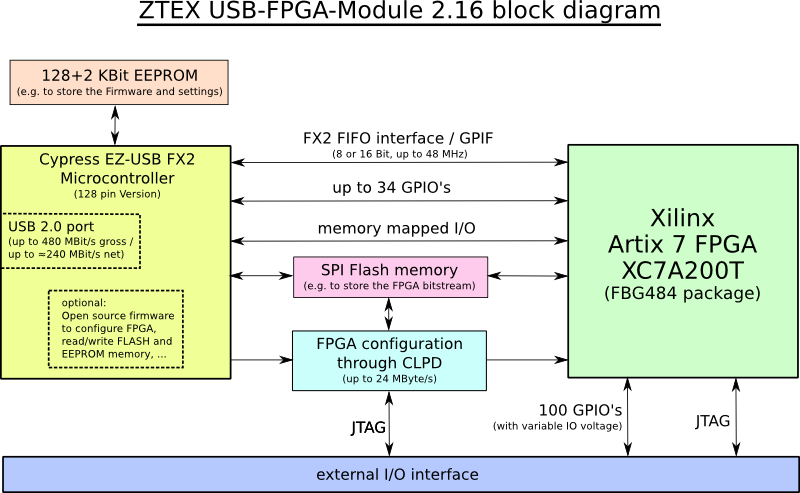
\includegraphics[width = 0.8\textwidth]{figures/usb-fpga-216.png}
	\caption{A ZTEX 2.16 FPGA board felépítése} 
	\label{fig:ztex_block}
\end{figure}

\todo[inline]{Képhiba}

Ezen felül a rajta található Xilinx Artix 7 FPGA megfelelő hűtését is biztosítja a panel. Az FPGA főbb datai \aref{table:artix7spec} táblázatban láthatóak. Ez az eszköz a Xilinx jelegelg kereskedelemi forgalomban kapható egyik zászlóshajója, amit bizonyít is a ZTEX panel 500 Eurós vételára.

\begin{table}[]
\centering
\begin{tabular}{ll}
Logikai cellák               & 215360 \\
Szeletek                     & 33650  \\
CLB Flip-flopok              & 269200 \\
Eloszott memória (kb)        & 2888   \\
Blokk RAM/FIFO (36 kb/darab) & 365    \\
Blokk RAM összesen (kb)      & 13140  \\
                             &        \\
                             &        \\
                             & 
  
\end{tabular}
\caption{A Xilinx Artix 7 XC7A200T}
\label{artix7spec}    
\end{table}

Bár a jelenlegi modell mindössze 10\%-át foglalja le a teljes hardwarenek, a későbbi bővülésre is hagy lehetőséget. A fimware elkészítésére és fejlesztésére a Xilinx Vivado környezet biztosít lehetőséget. Ebben készült el a keretrendszer, mely a Simulinkból generált HDL fájlokat tudja fogadni, megfelelő interfészen keresztül a kártyára vezetni.


\subsection{Szigma-Delta (\Sigma\Delta)\ átalakítók}

Az FPGA nem rendelkezik analóg kiementekkel, azonban a CCB számára elő kell állítani a normál működés során visszamért analóg jeleket, hiszen ebben relik a szimulátor lényege, a vezérlő elektronika szmszögéből nincsen különbség a valós hardware és a szimulátor között. A szigma delta átalakító nagyon nagy vonalakban egy órajel és egy fix impulzusszélességű négyszögjel, mely vagy logikai egy értéket, vagy logikai nulla értéket vesz fel az órajel minden felfutó (vagy lefutó) élére. Az így kialakult impulzusjel kitöltési tényezője egy hosszabb mintavételi ablakot tekintve arányos a bemeneti kódszóval. Ezek után a jelet egy az órajelnél sokkal kisebb vágási frekvenciájú aluláteresztő szűrűvel feldolgozva analóg jelet kapunk. A szigma delta átalakító további odo{vagy további, vagy rendes összehasonlítás} előnye a PWM kimenethez képest, hogy a kvantálái zajt nagyfrekvenciás tartományba tolja.\cite{artofelectronics}

\todo[inline]{PWM vs sigma delta spektrum}

Igen félrevezető névvel szokás "1 bites DA" átalakítónak is nevezni. A kifejezés egyszerűséget és alacsony teljesítményt sugall, ennek ellenére a megoldás rendkívül lineáris és nagy felbontású eredményt ad, így elterjedten használják pl. audio eszközökben is.

A mi esetünkben két részre bontható az átalakító. A modellben fut egy analógjelből digitális jelet létrehozó szigma-delta átalakító, majd az így kiadott digitális jelet szűrjük már az FPGA-n kívül egy aluláteresztő szűrűvel. \Aref{fig:sigmadelta} ábra szemlélteti az átalakító működését. A bejövő analalóg jelből levonjuk a hibajelet, majd egy komparátor összehasonlítja egy referenciával. Amennyiben nagyobb a bejövő jel, a kimenet logikai "1" értéket vesz fel, ha kisebb, logikai "0"-t. Ezt a jelet, egy 1-bites DAC-on keresztül vezetve akkumuláljuk, így kialakítva a hibajelet. 

\begin{figure}[!h]
	\centering
	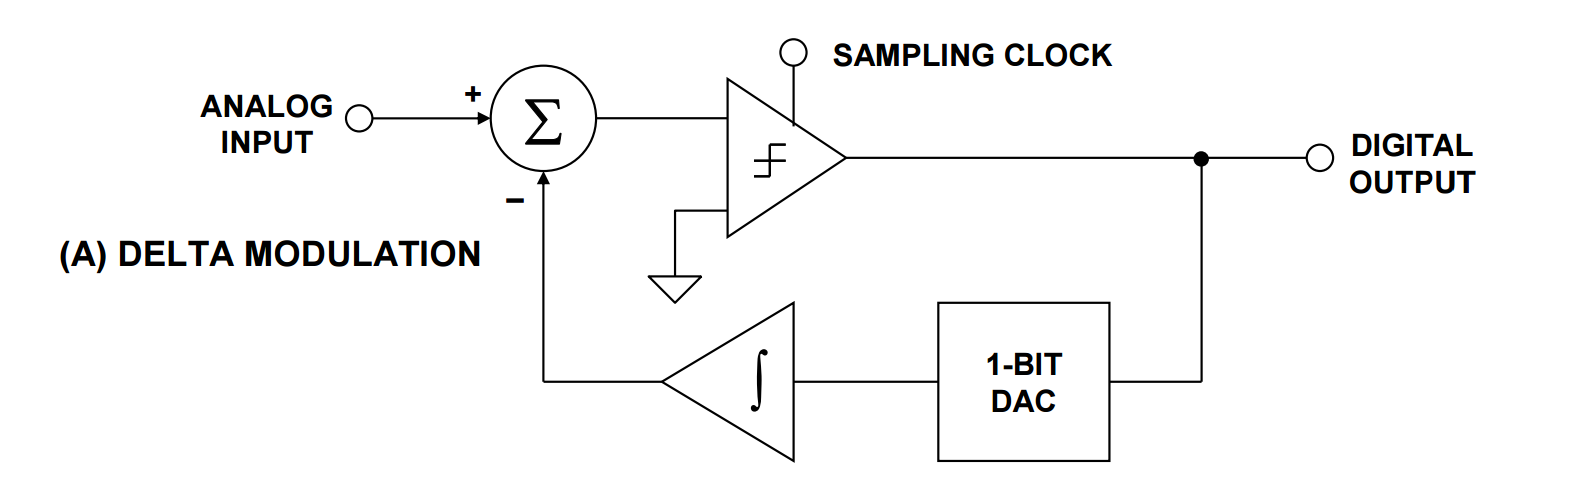
\includegraphics[width = 0.75\textwidth]{figures/sigmadelta.png}
	\caption{A szigma-delta átalakító} 
	\label{fig:sigmadelta}
\end{figure}

Az így kapott jelet már a modellből az FPGA lábára vezethetjük. Mivel az FPGA kiemeneti bankjainak feszültsége maximum $3,3\ V$, ezért a szűrés után erősítésre is szükség lehet.

\begin{figure}[!h]
	\centering
	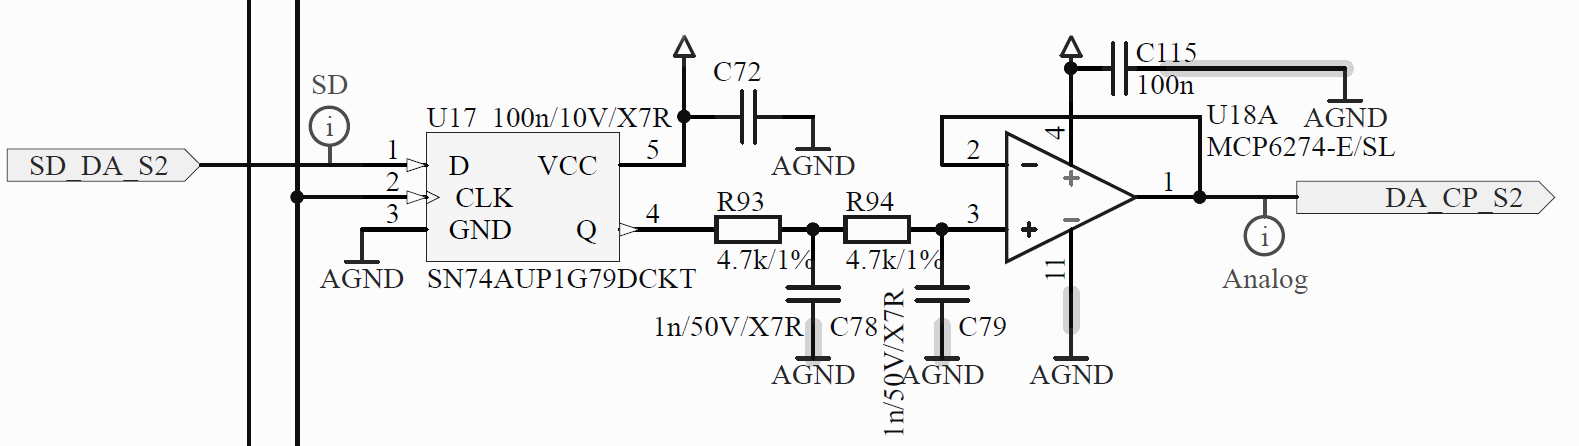
\includegraphics[width = \textwidth]{figures/lowpassfilter.png}
	\caption{A négyszögjelet fogadó aluláteresztő szűrő} 
	\label{fig:lowpass}
\end{figure}

\Aref{fig:lowpass} ábrán látható aluláteresztő szűrő kimenet már közvetlenül a CCB analóg bemenetére csatalkozik. A CCB analóg mérései differenciálisak a valóságban, mivel a valós enelktronikában sokkal nagyobb zaj éri a rendszert. A modellen azonban ez a zavar nem jelentős, így a mérés negatív jelét földre kötjük.

\section{Simulink modell}

A futtatandó modell magában foglalja a teljesítményelektronikai elemek modelljét, egy motor modellt és egy mechanikai terhelés modellt. Hiányossaág volt a modellnek, hogy a DC link feszültésge egy konstans érték volt, így a különböző terhelések DC feszültségre való visszahatásást nem lehetett vizsgálni. További hiányosság, hogy a hálózat paramétereit sem vette így figyelembe a modell.

\subsection{A rendelkezésre álló modell}

\Aref{fig:original_model}. ábrán látható a korábban elkészített modell és az egyes blokkok kapcsolata. Jó kiniduló alapot biztosított, jól megfigyelhető rajta a rendszer működése. Ez a modell bemenetként tekint a DC feszültségre, így az én bemeneti modellemet ezen kívül helyeztem el. A terhelés a bemeneti modellben DC terhelőáram formájában jelentkezik, így ezt a jelet elő kellett még állítani. A rendelkezésre álló félhíd modell csak az AC áramot állítja elő kiemenetként, így ezt módosítani kellett, hogy a DC áram is előálljon. Ezek után a három félhíd áramát összegezve felhasználhatóvá vált az I_{DC} terhelőáram, bemenetként a DC kört is tartalmazó modellemnek.


\begin{figure}[]
	\centering
	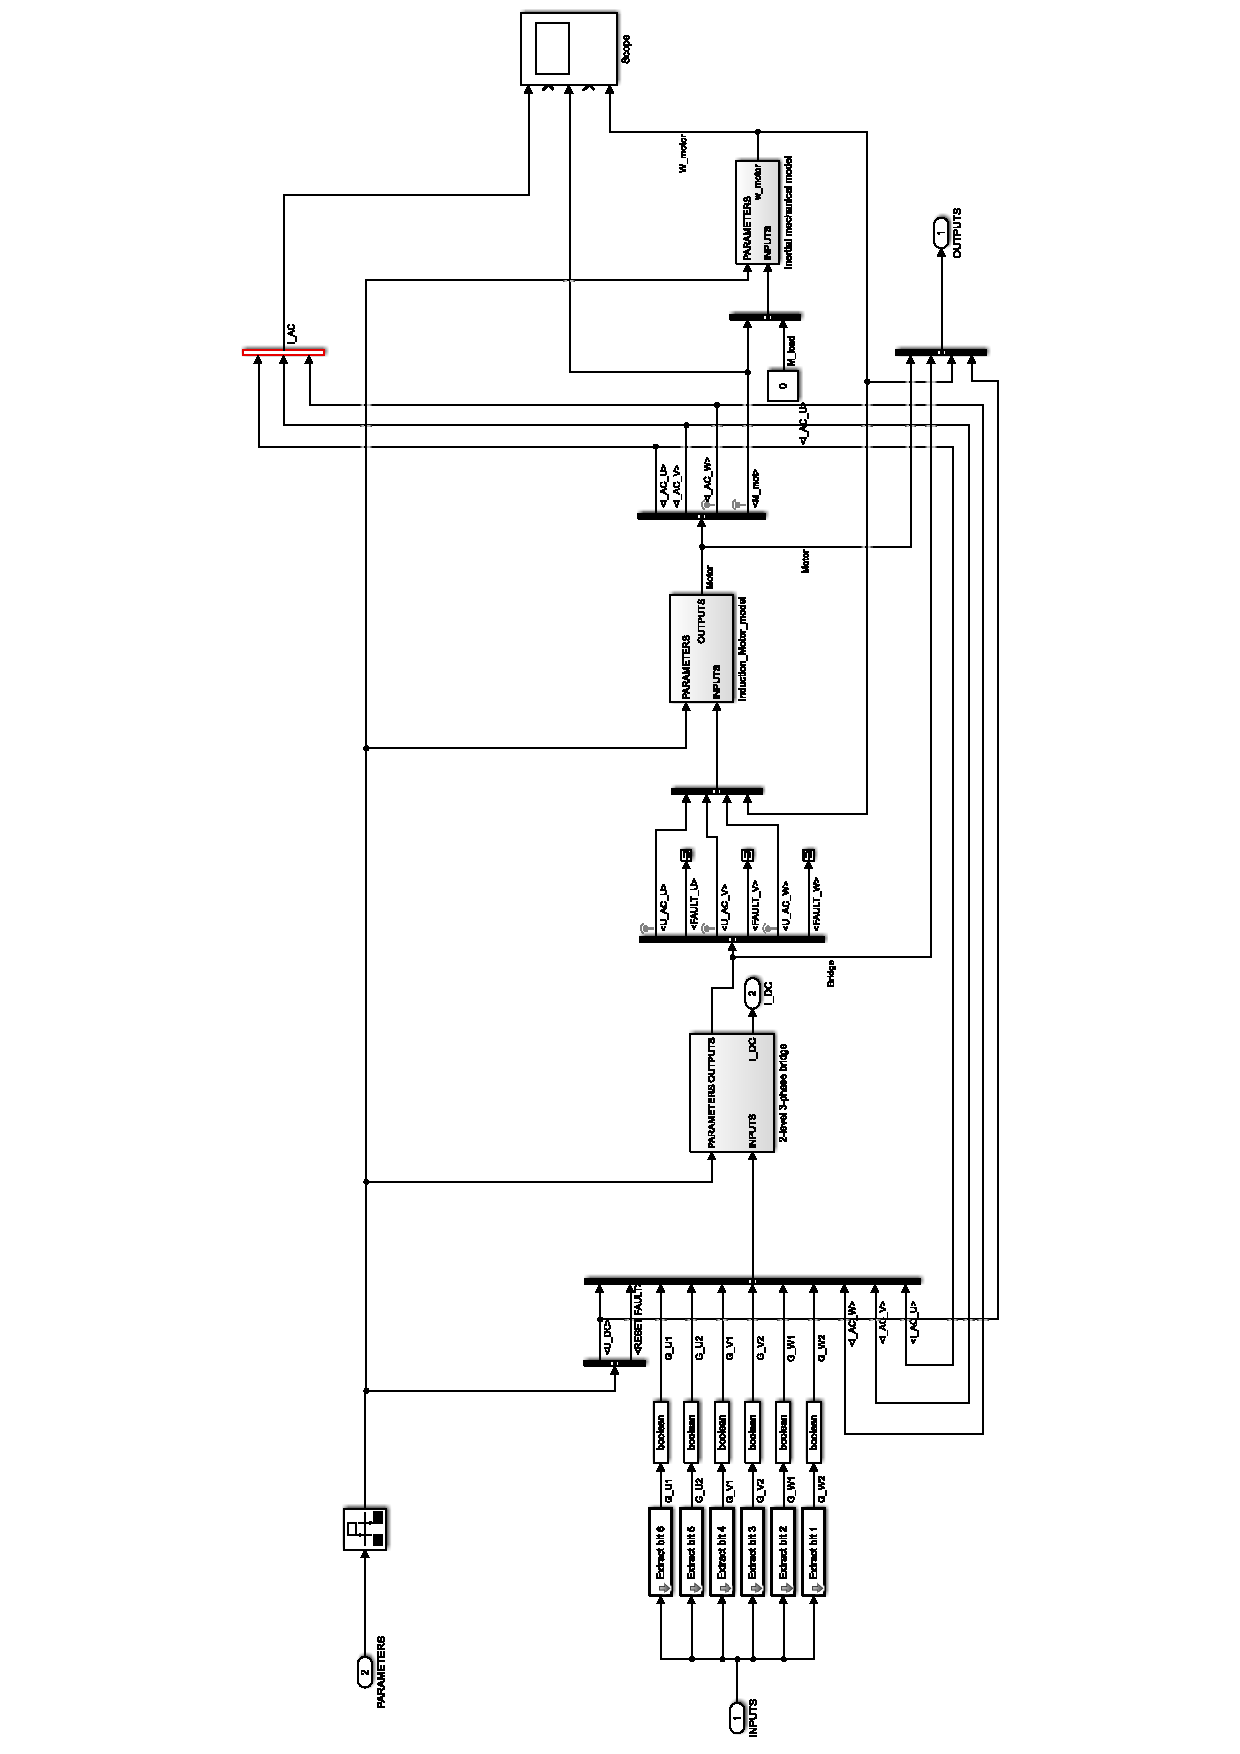
\includegraphics[width = \textwidth]{figures/hil_model.pdf}
	\caption{A SIMULINK model} 
	\label{fig:original_model}
\end{figure}

Az I_{DC} terhelőáramot az alábbi egyenletek segítségével határozhatjuk meg:

\begin{equation}
\centering
$$
I_{DC}
=
\begin{cases}
I_{AC}   & ha \  PWM_H = 1 \  | \  PWM_H = 0 \  \& \  I_{AC} < 0 \\
0 & 
\end{cases}
$$    
\end{equation}

A módosítások \aref{fig:igbt_model}. ábra alsó részén láthatóak. Ebből a modellből valóstja meg együttesen három darab az inverter kimeneti fokozatának modelljét. 

\begin{figure}[]
	\centering
	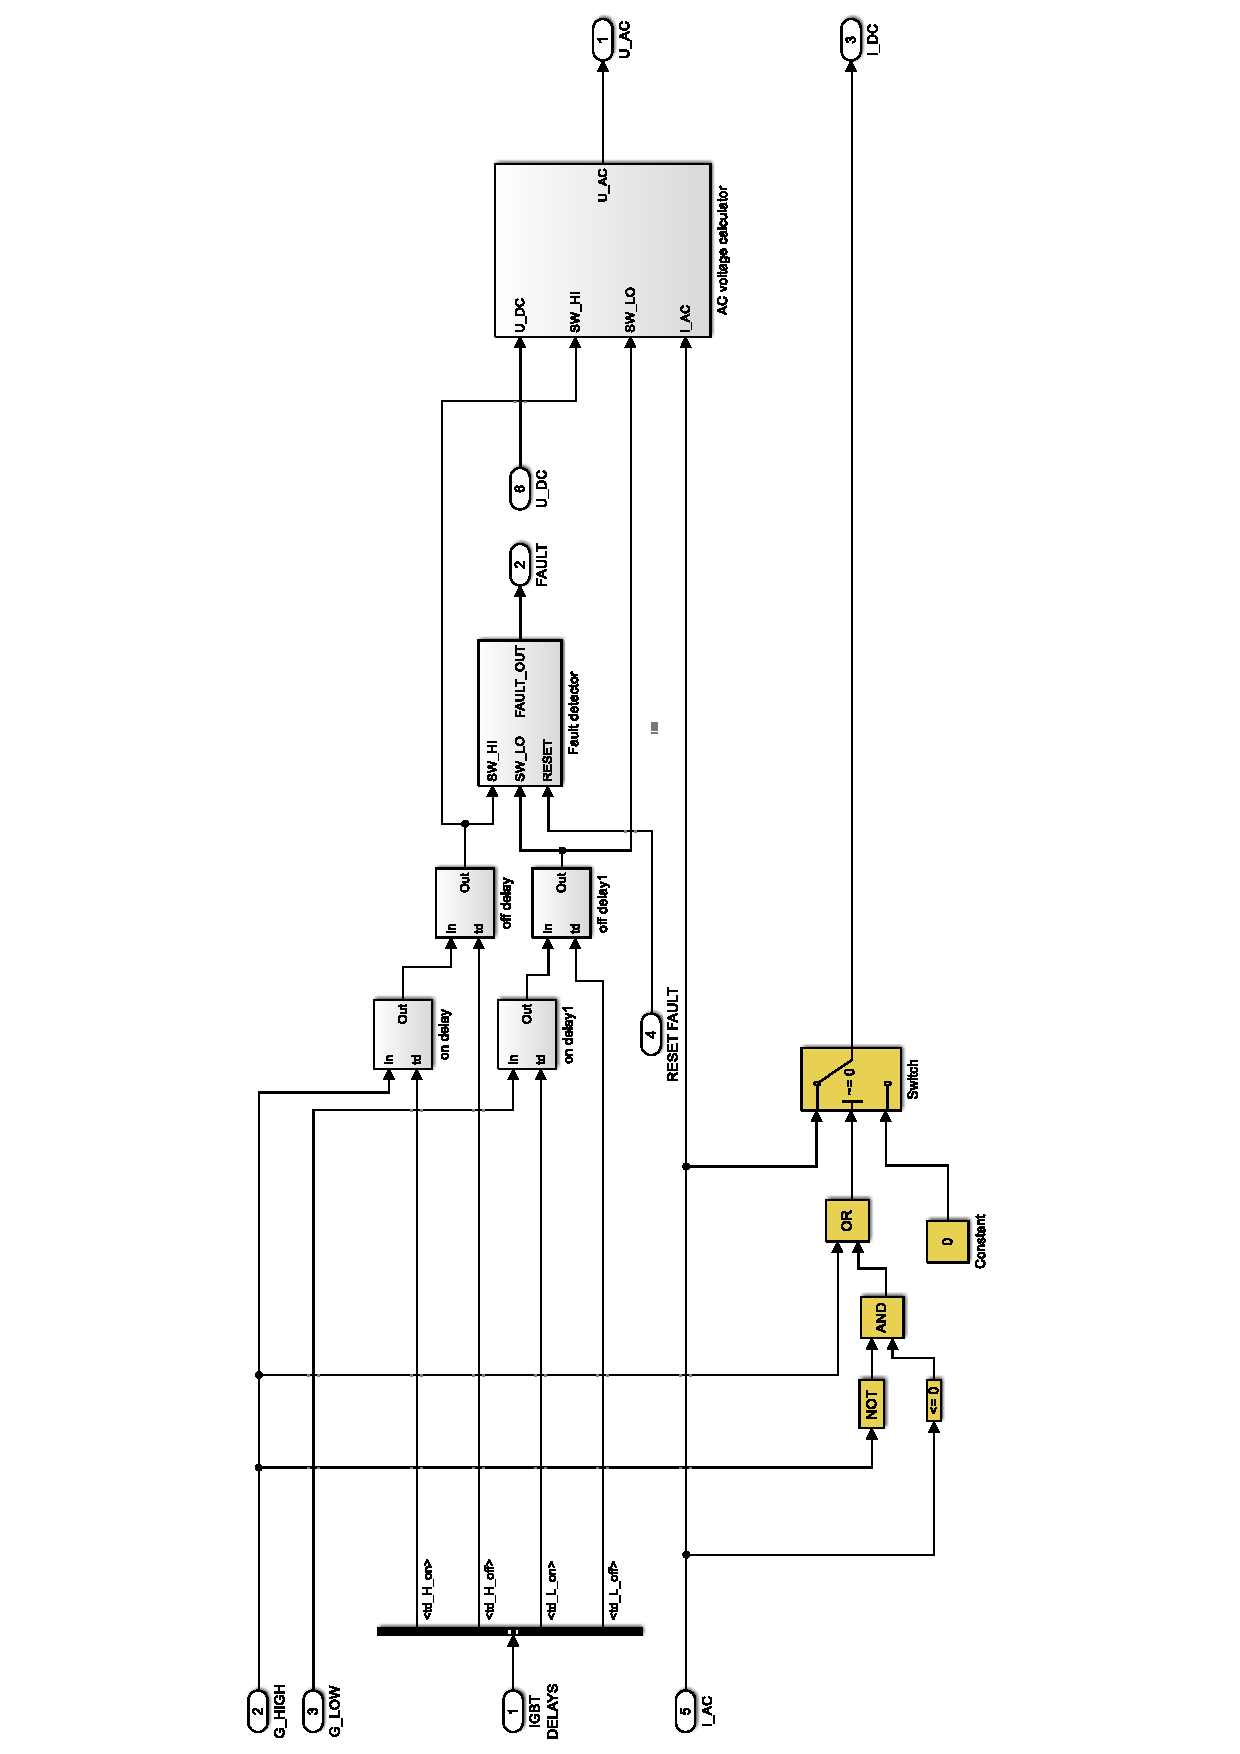
\includegraphics[width = \textwidth]{figures/igbt_model.pdf}
	\caption{A módosított félhíd modell} 
	\label{fig:igbt_model}
\end{figure}




\subsection{Az implementált bemeneti modell}

\begin{figure}[]
	\centering
	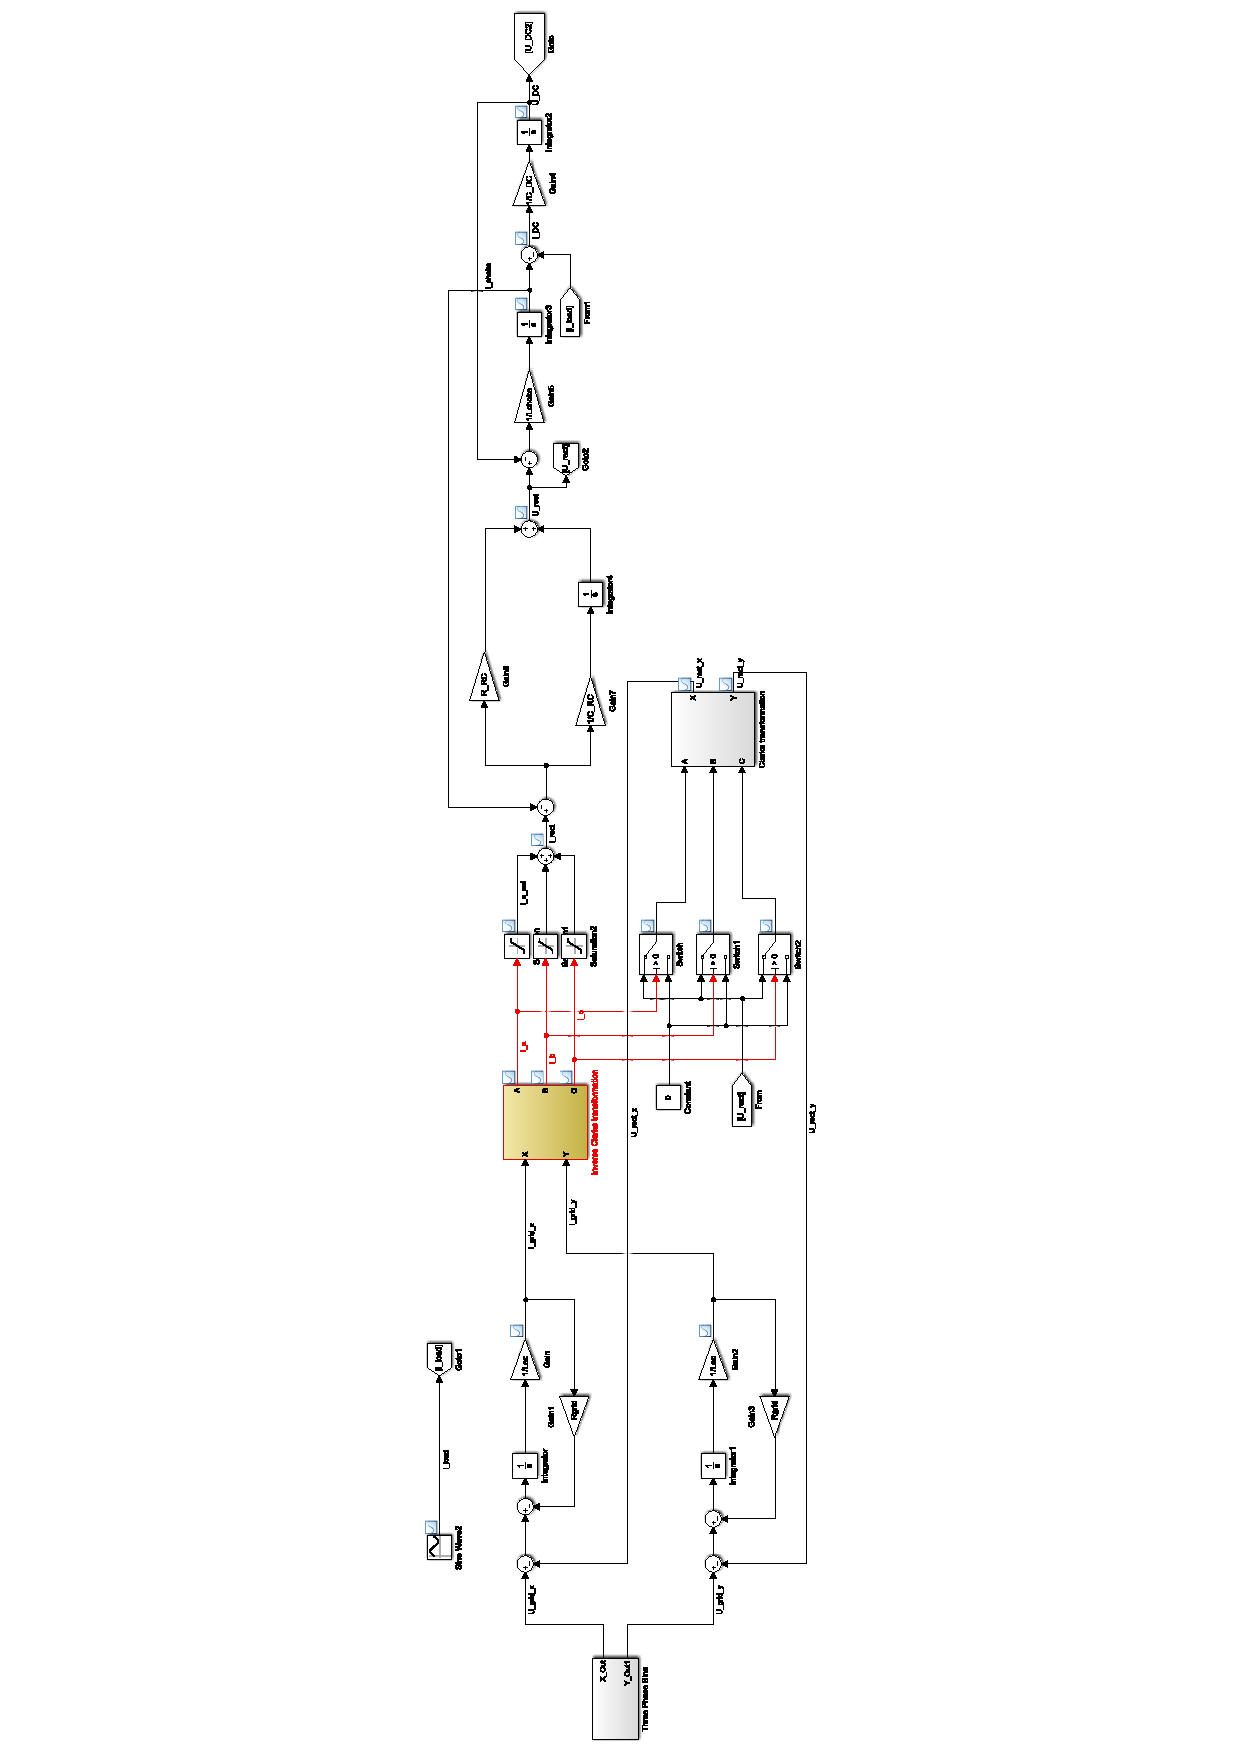
\includegraphics[width = 1.2\textwidth]{figures/model_continous.pdf}
	\caption{A frekvenciaváltó bemenetének folytonos modellje} 
	\label{fig:cont_input_model}
\end{figure}

A feladat tehát az volt, hogy a korábbi modellt egészítsem ki egy olyan blokkal ami a felsorolt hiányosságokat orvosolja. Az elkészítendő modellnek tartalmaznia kell tehát egy háromfázisú hálózatmodellt, a diódás hidat, a bemeneti DC folytót, illetve a DC link kondenzátort. A modellezendő főáramkori részt \aref{fig:input_marked} ábrán jelöltem. 

\begin{figure}[H!]
	\centering
	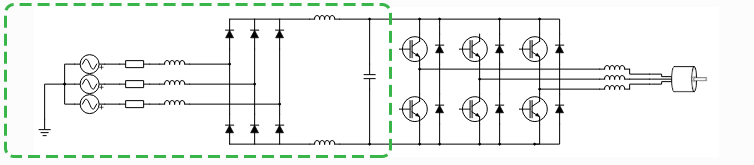
\includegraphics[width = \textwidth]{figures/VFDschematic_choke_marked.png}
	\caption{A frekvenciaváltó bemenetének folytonos modellje} 
	\label{fig:input_marked}
\end{figure}

Az első lépés a hálózat modellezése. Ehhez szükségünk van egy szinuszos feszültség előállítására. Mivel a hálózatot egy soros RL modell adja, melynek átviteli függvénye az alábbi. 

\begin{equation}
I(s) = \frac{U(s)}{R+Ls}
\end{equation}

Mivel a három fázis induktivitása nem független egymástól, ezért az egyes fázisok egymásra hatását is fogyelembe kell venni a szimuláció során. Ez jelentős számításbeli töbleetet jelenteni, a modell struktúráját is bonyolítaná, ezért a fázisokat inkább szétcsatoljuk és az $x,y$ koordinátarendszerben ábrázoljuk őket. Emiatt a szinusz generátor modulban máregyből egy sinust és cosinust hozunk léra, azaz két szinusz hullámot, $90°$ fáziskülönbséggel. Ezt a két jelet vezetjük át egy-egy R-L blokkon megkapva így a hálózati áramokat. Azért, hogy visszakapjuk a háromfázisú mennyiségeket, inverz Clarke transzoformációt alkalmazunk a két jelent, ígyelőáll a három fázis árama, mely a diódás híd bemenetéül szolgál.

\begin{equation}
\centering
\begin{bmatrix}
       U_a\\[0.3em]
       U_b\\[0.3em]
       U_c          
\end{bmatrix}
=
\begin{bmatrix}
       1 & 0 & 1  \\[0.3em]
       -\frac{1}{2} & \frac{\sqrt{3}}{2} & 1  \\[0.3em]
       -\frac{1}{2} & -\frac{\sqrt{3}}{2} & 1 
\end{bmatrix}
\begin{bmatrix}
       U_x\\[0.3em]
       U_y\\[0.3em]
       U_0,,        
\end{bmatrix}    
\end{equation}

\begin{equation}
\centering
\begin{bmatrix}
       U_x\\[0.3em]
       U_y\\[0.3em]
       U_0 
\end{bmatrix}
=
\begin{bmatrix}
       \frac{2}{3} & -\frac{1}{3} & -\frac{1}{3}  \\[0.3em]
       0 & \frac{1}{\sqrt{3}} & -\frac{1}{\sqrt{3}}  \\[0.3em]
       \frac{1}{3} & \frac{1}{3} & \frac{1}{3}    
\end{bmatrix}
\begin{bmatrix}
       U_a\\[0.3em]
       U_b\\[0.3em]
       U_c    
\end{bmatrix}
\end{equation}

A Clarke transzformáció arra szolgál, hogy egyszerűsítsük a háromfázisú rendszerekben elvégzendő számításokat, mivel a három jellemző mennyiséget csupán kettővel reprezentálja. További előnye, hogy a nulla sorrendű komponensek a számítások során kiesnek, amire jelen esetben csak akkor lenne szükségünk, ha földzárlatot is kívánnánk szimulálni.

A didódás modell nagyon leegyszerűsített, csak azon üzemállapotát reprezántálja a 3 fázisú 2 utas, 6 ütemű egyenirányítónak, amikor két dióda vezet benne. Ezt pedig úgy valósítjuk meg, hogy mind a három fázis negatív tatományát levágjuk, ezek után pedig az áramok összegezhetővé válnak, így előállítva az $I_{rect}$ egyenirányított áramot. A diódákon eső feszültséget pedig úgy állítjuk elő, hogy ahhoz a diódához, amelyik éppen vezet, hozzárendeljük az $U_rect$ egyenirányított feszültséget. A hálózatra való visszahatás kiszámításához azonban az így kapott háromfázisú mennyiséget vissza kell alakítanunk $x,y$ tartomány beli mennyiségekké, erre szolgál a Clark traszformáció.

Ezen a ponton két problémába is ütközünk: a didás hídnak nincs olyan állapota ,hogy egyik dióda sem vezet, emiatt a DC kondenzátorunk a végelenségig töltődik. A jövőben tervezem a modell további finomításást, ehhez egy állapotgépet kell majd megvalósítani, a modell demonstrációs jellegére való tekintettel azonban most mást megoldást válaszottam. Empirikus úton kiderül, hogy a kondenzátort minimum $350\ mA$-el terhelni kell, hogy ne inegrálódjon el, hanem stabilizálódjon az értéke.

A msáik probléma abból adódik, hogy DC fojtó modelljének feszültség bementere van szüksége, és áram kimenetet ad, a diódás hídnak pedig áram kimenete van. Más struktúrájú modellel lehetséges így is megvalósítani a szimulációt, azonban egyszerűbb szétválasztani ezeket az állapotávltozókat egy virtuális RC-tag bevezetésével. Ennek segítségével az egyenirányító és a fojtó között is megjelenik a modellben egy potenciál. Az RC-tag paramétereit úgy választjuk meg, hogy az a modell valós működésést ne befolyásolja. Úgy is tekinthetünk erre a tagra, mint egy PI szabályzóra, mely az induktivitáson eső feszültséget igyekszik $0$-ra szabályozni, felvéve a DC-link kondenzátor feszültségét.

\begin{figure}[H!]
	\centering
	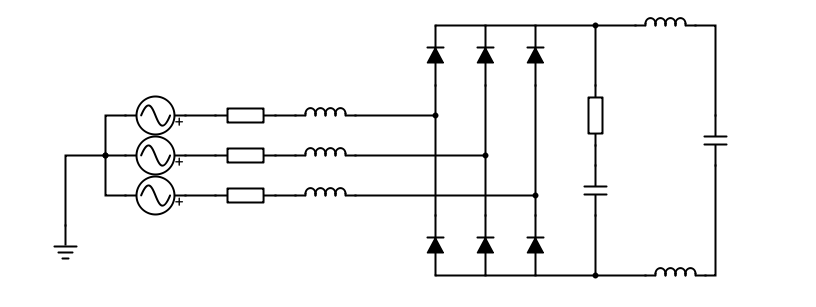
\includegraphics[width = \textwidth]{figures/VFD_virtual_RC.png}
	\caption{A frekvenciaváltó modellezett szakasza} 
	\label{fig:virtualRC}
\end{figure}

Ez így kiszámolt áramból kivonva a terhelés áramát meg kapjuk a DC kondenzátort töltő áramot.

Az így kialakult modell paraméterei \aref{tab:parameters}. táblázatban láthatóak. A DC fojtó induktivitását úgy kell érteni, hogy a valós rendszerben a negatív és a pozitív sínen is van egy-egy fojtó, azonban a modellben ez a kettő egyesítve van.

\begin{table}[H]
\centering
\begin{tabular}{lS}
Hálózati feszültség            & $325\ V$ 		\\
Hálózati ellenállás            & $2\ m\Omega$   \\
Hálózati induktivitás          & $20\ \mu{}H$    			\\
DC fojtó induktivitása         & $2 \cdot{} 3\ mH$    			\\
DC link kondenzátor kapacitása & $270\ \mu{}F $   
\end{tabular}
\caption{A modell paraméterei}
\label{parameters}
\end{table}

\begin{figure}[H]
	\centering
	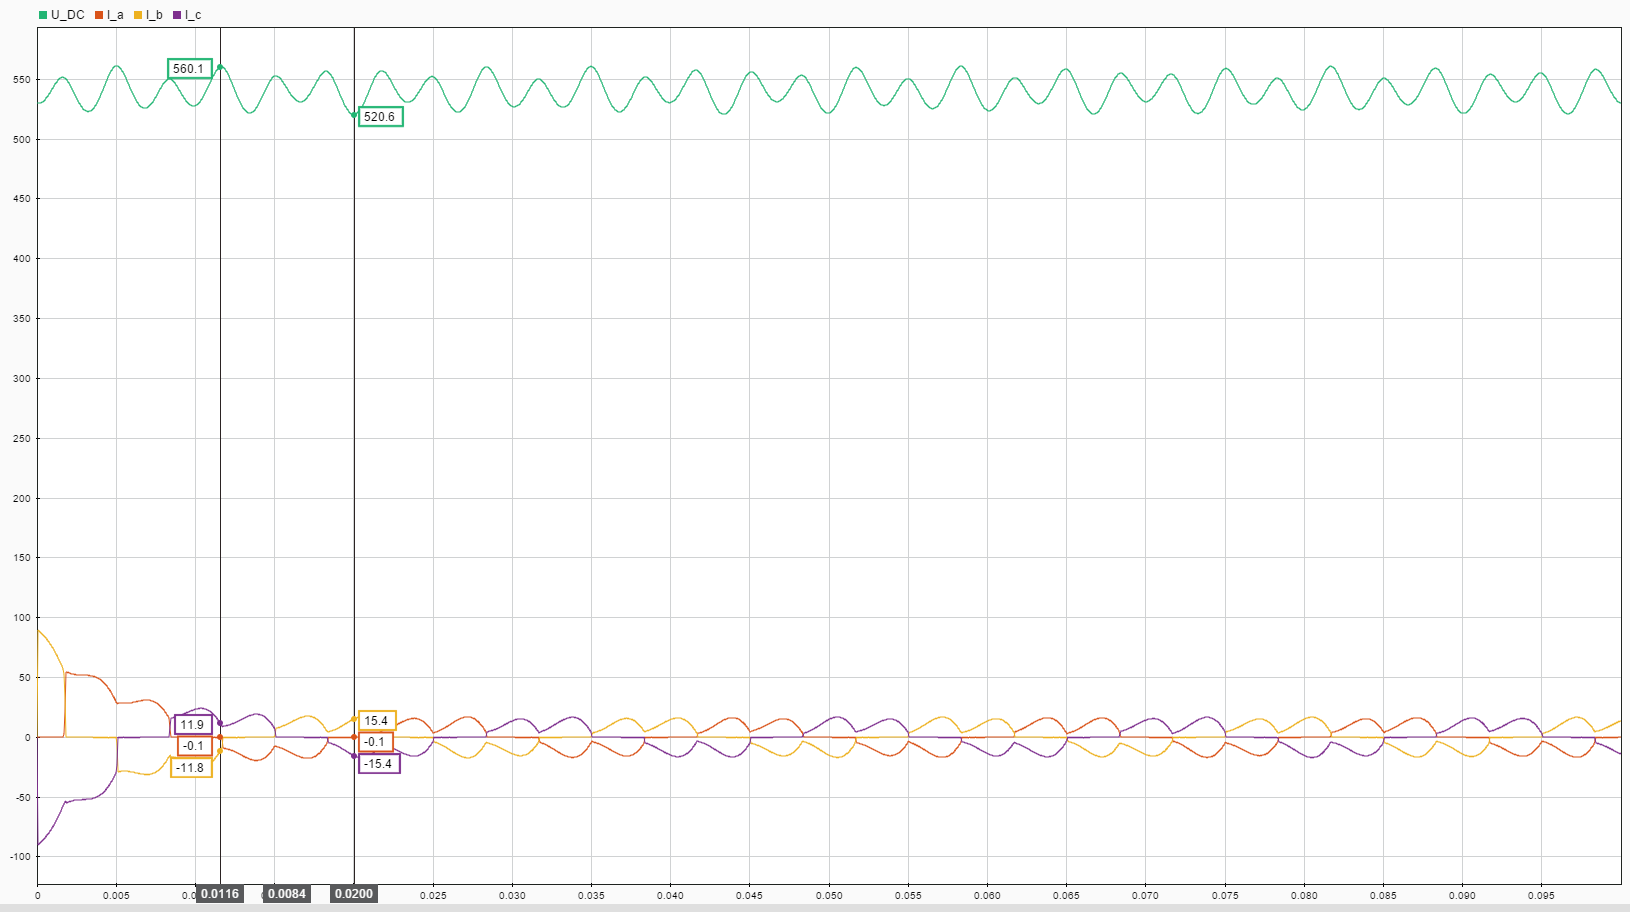
\includegraphics[width = \textwidth]{figures/continous_testrun_1.png}
	\caption{A frekvenciaváltó modellezett szakasza} 
	\label{fig:cont_run}
\end{figure}

\subsection{A DC fojtó szerepe}

A frekvenciaváltók bemeneti fokozatára vagy DC vagy AC oldalon szokásos fojtót alkalmazni. 

\begin{figure}[H!]
	\centering
	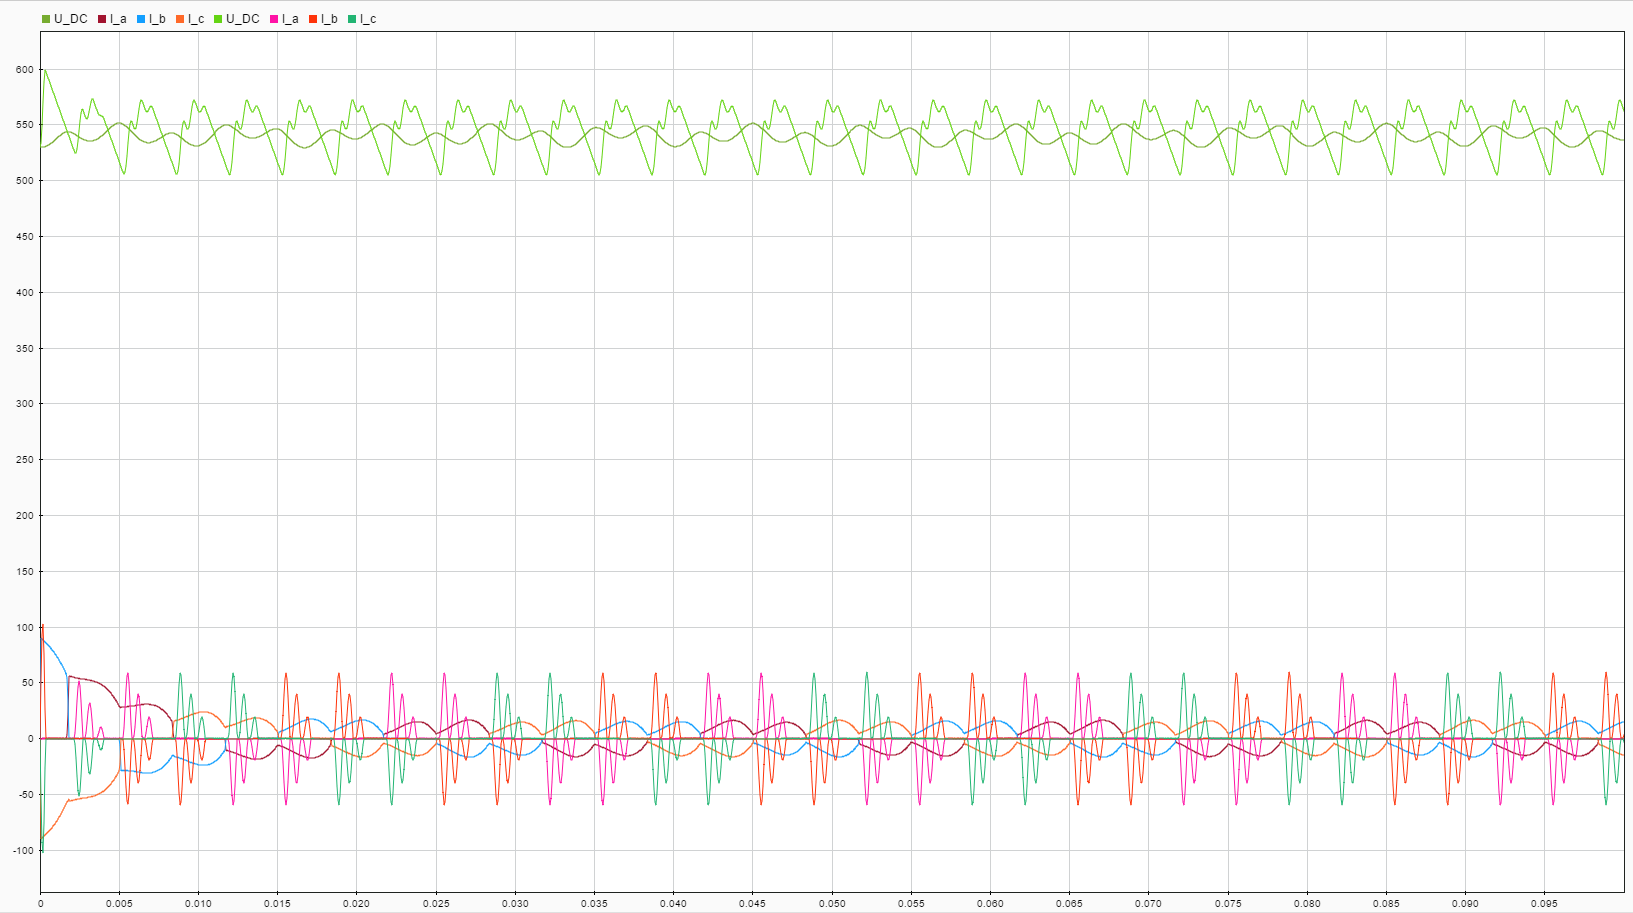
\includegraphics[width = \textwidth]{figures/choke_vs_nochoke_11A.png}
	\caption{A DC fojtó szerepe} 
	\label{fig:cont_run}
\end{figure}



\subsection{Áttérés diszrét időre}

Az eddig mevalósított hálózatmodell folytonos idejű, Laplace tartományban ábárzolt egyenletekkel. Az FPGA, mint minden digitális rendszer azonban diszkrét időben fogja ezeket megoldani. Emiatt a modellt át kell traszformálni \emph{z} tartományba. Az integrátor matematikailag az alábbi alaknak felel meg:

\begin{equation}
\centering
\frac{1}{s} \Rightarrow \frac{1}{1-z^{-1}}
\end{equation}

Ez az átalakítás a modellben grafikusan pedig az alábbi módon jelentkezik:

\begin{figure}[h]
	\centering
	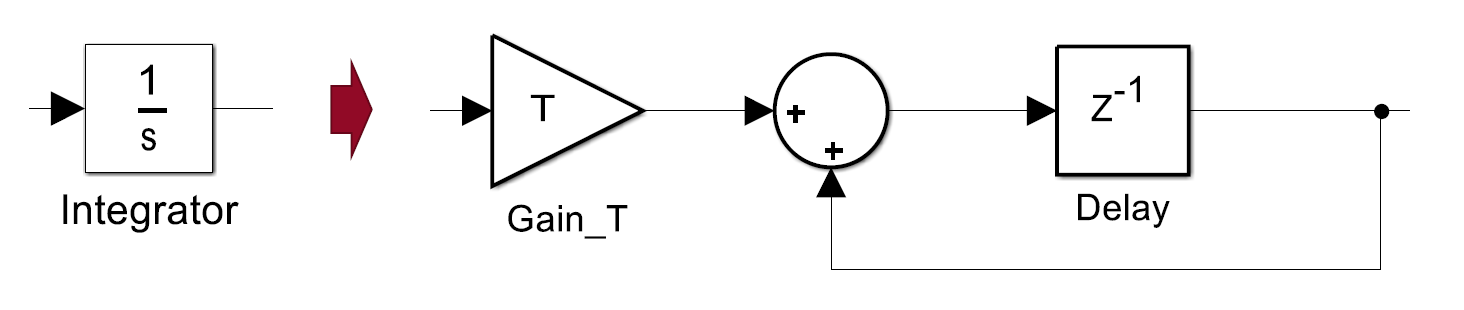
\includegraphics[width = \textwidth]{figures/integrator.png}
	\caption{Az integrázor diszkrét idejű megvalósítása} 
	\label{fig:integrator}
\end{figure}

Tehát az összes integrátor blokkon el kell végezni a fenti átalakítást.

\todo[inline]{Itt még ki kéne egészíteni z tartomány beli rizsával}

\subsection{Fixpontos ábárzolás}

Az FPGA-ban hatékonyan csak fixpontos aritmetika valósítható meg, így a most lebegőpontos változóinkat át kell alakítanunk fixpontosra. Ez könnyen megoldható, hiszen az egyes változók értéktartománya előre ismert, pl tudjuk, hogy a DC feszültség biztosan kisebb, mint $U_{DC}=1000\ V$.

A lebegépontos számábárolás megkülönböztet egyszeres (floating) és kétszeres (double) precizitást. Előbbi a számot 32 utóbbi pedig 64 biten tárolja.

\begin{figure}[H]
	\centering
	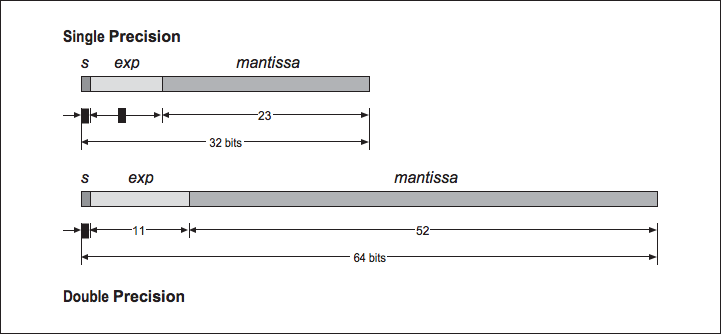
\includegraphics[width = 0.8\textwidth]{figures/floating.png}
	\caption{A lebegőpontos számábrázolás} 
	\label{fig:floating}
\end{figure}

Ilyen módon a floating körülbelül 7, a double pedig 17 tizedesjegy pontosságot enged meg. Mindkét ábrázolásmód 1 darab előjel bitet után mantissza és exponens formájában tárolja a számot. A mantissza normál alakban, a kettedespont mögötti biteket tárolja. A normálak biztosítja, hogy a kettedespont előtt már csak garantáltan 1 darab 1-es van, így ez elhagyható. Az exponens pedig egy a kettedespont helyét tárolja úgy, hogy a valós kitevő 127-el csökkentve van.

A fixpontos ábrázolás ezzel szemben rögzíti a tizedespont helyét, valamint azt nem kódolja a változóban, hanem a típusa határozza meg az értelmezés módját. A MATLAB-nak saját fixpontos formátuma van, melyet a \emph{fixdt(s,b,f)} formátummal használhatunk. Az \emph{s} jelöli, hogy az adott szám előjeles-e vagy sem, ha 1 az értéke akkor igen, ha 0, akkor nem. A következő \emph{b} a bitek számát jelöli összesen, theát itt adhatjuk meg, hogy hány biten legyen ábrázolva a szám. Ha az adott szám előjeles, akkor nem adódik hozzá a mérethez még egy bit az előjel miatt, hanem 1 bittel csökken a szám tárolására felhasnználható hely. Az utolsó \emph{f} szám jeleni a kettedesjegyek számát. Néhány példa \aref{tab:fixdt}. táblázatban látható. 

\begin{table}[]
\centering
\begin{tabular}{|l|l|l|}
\hline
MATLAB típus  & tartomány               & LSB \\ \hline
fixdt(0,32,0) & 0..4294967296           & 1   \\ \hline
fixdt(1,32,0) & -2147483648..2147483648	& 1   \\ \hline
fixdt(0,8,10) & 0..0,25        	   	    & 0,0009765625 \\ \hline
fixdt(0,8,8)  & 0..1     			 	& 0,00390625    \\ \hline
fixdt(1,8,2)  & -31..32     			& 0,25    \\ \hline
\end{tabular}
\caption{A MATLAB fixpontos formátumai}
\label{tab:fixdt}
\end{table}

A Simulink alapbeállításként double változóként hozza létre a jeleket és dolgozik velük. Az FPGA-val való kompatibilitás miatt azonban át kell étrni fixpontos ábárzolásra. Ennek a feladatnak a megkönnyítésére a MATLAB tartalmazza a \emph{Fixpoint Advisor} nevű eszközt, azonban ilyen kis méretű modell esetében az eszköz jó felparaméterezése tovább tarthat, mint maga a megvalósítás. Az egyes változók határai látszanak a vizsált értéktartományból. Ezen felül korlátot jelet még maga a hardver, mivel az FPGA maximum egy 18 és egy 25 bites számot tud összeszorozni. A mayimumális bitszám miatt tehát a pontosság és az ábrázolható értéktartomány között kell megtalálni az egyensúlyt.

\begin{table}[]
\centering
\begin{tabular}{|l|l|l|}
\hline
Jel  					&		 tartomány              & választott adattípus \\ \hline
Hálózati feszültség (V) & -1000-1000          	 		& fixdt()\\ \hline
Hálózati áram (A) 		& -50..50						& fixdt()\\ \hline
DC áram 				& -50..50        	   	   		& fixdt() \\ \hline
DC feszültség  			& 0..1000     			 		& fixdt(0,18,6)    \\ \hline
\end{tabular}
\caption{A vizsgált jeltartományok}
\label{tab:values}
\end{table} 

A kezdeti értékek meghatározása után azonban a modellen belüli számítások elvégézéséhez is meg kell találnunk a megfelelő típusokat. Ennek érdekében célszerű megvizsgálni, hogy az egyes műveletek milyen változást okoznak az ábrázolandó tartományban.

Összeadás esetén ha fixdt(1,n,f1) és fixdt(1,n,f2) típusú számokat adunk össze (f1 < f2), esetén el kell dönteni, hogy a pontosság csökkenhet-e. Amennyiben igen, használhatjuk a továbbiakban a kevesebb törtrész bitet használó típust. Ha nem engedhető meg az ábárzolás pontosságának csökkenése fixdt(1,n+f1-f2,f1) típust kell választani kimenetként. Bár a táoláshoz szükséges bitek száma megnő, nem történik sem túlcsordulás és nem vesztünk az ábrázolási pontosságból sem.

Szorzás esetén az eredményhez szükséges bitek számának változását az operandus kettes alapú logaritmusával számíthatjuk. A törrész bitek száma $-log_2\abs{a} = m$ bittel nő a törtrész bitek száma.

Integrálás esetén ütközünk jelentősebb problémába (és a Fixpoint Advisor is itt vérzik el), mivel ebben az esetben nagyon kis számokat kell akkumulálni. A folytonos összegzés miatt az eredmény nagyra nőhet, a pontosságot azonban úgy kell megválasztnai, hogy ábrázolható legyen az inkrement. Szerencsére összeadni több biten is lehet az FPGA-ban, így nem okoz problémát nagyobb típust váalsztani, azonban az integrátor után vissza kell konvertálni 18 biten ábrázolható méretre, még ha ezzel a pontossábgól veszítünk is.
\chapter{Miért FPGA?}
\section{Zynq vs. ZTEX}

yolo
\chapter{A Simulink modell felépítése}
\chapter{Működés és tesztek}


%%----------------------------------------------------------------------------
\chapter{\LaTeX-eszközök}\label{sect:LatexTools}
%----------------------------------------------------------------------------
\section{A szerkesztéshez használatos eszközök}
%----------------------------------------------------------------------------
Ez a sablon TeXstudio 2.8.8 szerkesztővel készült. A TeXstudio egy platformfüggetlen, Windows, Linux és Mac OS alatt is elérhető \LaTeX-szerkesztőprogram számtalan hasznos szolgáltatással (\figref{TeXstudio} ábra). A szoftver ingyenesen letölthető\footnote{A TeXstudio hivatalos oldala: \url{http://texstudio.sourceforge.net/}}.

\begin{figure}[!ht]
\centering
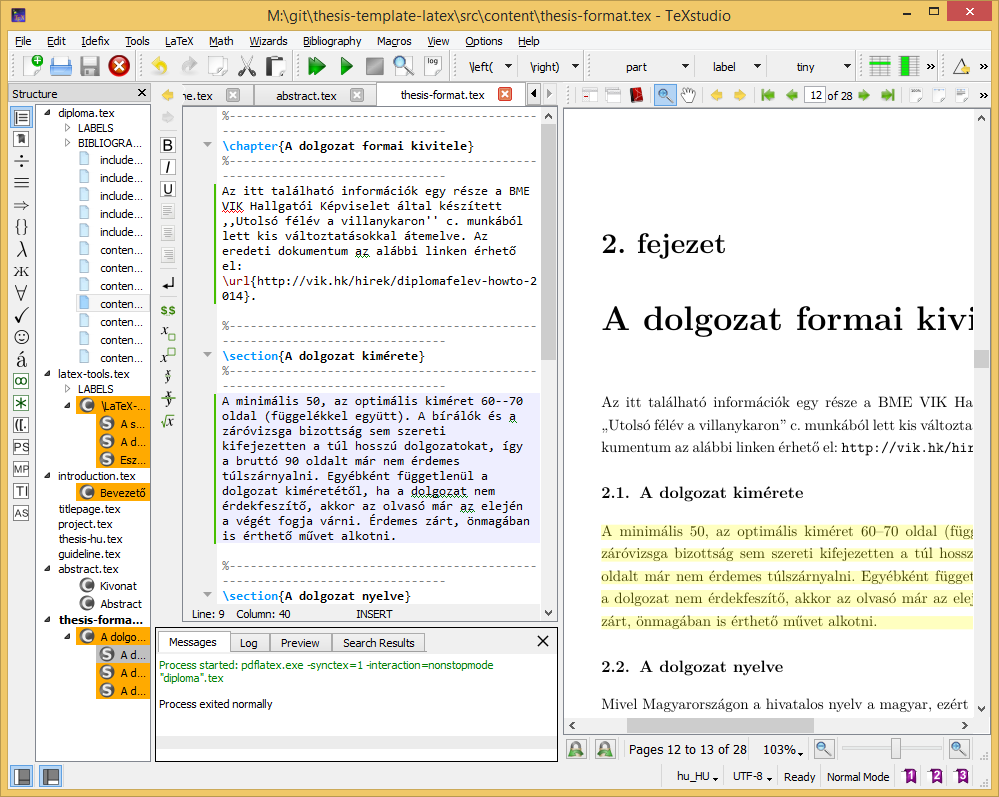
\includegraphics[width=150mm, keepaspectratio]{figures/TeXstudio.png}
\caption{A TeXstudio \LaTeX-szerkesztő.} 
\label{fig:TeXstudio}
\end{figure}

A TeXstudio telepítése után érdemes még letölteni a magyar nyelvű helyesírásellenőrző-szótárakat hozzá. A TeXstudio az OpenOffice-hoz használatos formátumot tudja kezelni. A TeXstudio beállításainál a \verb+General+ fülön a \verb+Dictionaries+ résznél tudjuk megadni, hogy melyik szótárat használja.

Egy másik használható Windows alapú szerkesztőprogram a LEd\footnote{A LEd hivatalos oldala: \url{http://www.latexeditor.org/}} (LaTeX Editor), a TeXstudio azonban stabilabb, gyorsabb, és jobban használható.

%----------------------------------------------------------------------------
\section{A dokumentum lefordítása Windows alatt}
%----------------------------------------------------------------------------
A TeXstudio és a LEd kizárólag szerkesztőprogram (bár az utóbbiban DVI-nézegető is van), így a dokumentum fordításához szükséges eszközöket nem tartalmazza. Windows alatt alapvetően két lehetőség közül érdemes választani: MiKTeX (\url{http://miktex.org/}) és TeX Live (\url{http://www.tug.org/texlive/}) programcsomag. Az utóbbi működik Mac OS X, GNU/Linux alatt és Unix-származékokon is. A MiKTeX egy alapcsomag telepítése után mindig letölti a használt funkciókhoz szükséges, de lokálisan hiányzó \TeX-csomagokat, míg a TeX Live DVD ISO verzóban férhető hozzá. Ez a dokumentum TeX Live 2008 programcsomag segítségével fordult, amelynek DVD ISO verziója a megadott oldalról letölthető. A sablon lefordításához a disztribúcióban szereplő \verb+magyar.ldf+ fájlt a \verb+http://www.math.bme.hu/latex/+ változatra kell cserélni, vagy az utóbbi változatot be kell másolni a projekt-könyvtárba (ahogy ezt meg is tettük a sablonban) különben anomáliák tapasztalhatók a dokumentumban (pl. az ábra- és táblázat-aláírások formátuma nem a beállított lesz, vagy bizonyos oldalakon megjelenik alapértelmezésben egy fejléc). A TeX Live 2008-at még nem kell külön telepíteni a gépre, elegendő DVD-ről (vagy az ISO fájlból közvetlenül, pl. DaemonTools-szal) használni. 

Ha a MiKTeX csomagot használjuk, akkor parancssorból a következő módon tudjuk újrafordítani a teljes dokumentumot:

\begin{lstlisting}[frame=single,float=!ht]
texify -p diploma.tex
\end{lstlisting}

A \verb+texify+ parancs a MiKTex programcsomag \verb+miktex/bin+ alkönyvtárában található. A parancs gondoskodik arról, hogy a szükséges lépéseket (fordítás, hivatkozások generálása stb.) a megfelelő sorrendben elvégezze. A \verb+-p+ kapcsoló hatására PDF-et generál. A fordítást és az ideiglenes fájlok törlését elvégezhetjük a sablonhoz mellékelt \verb+manual_build.bat+ szkript segítségével is.

A \TeX-eszközöket tartalmazó programcsomag binárisainak elérési útját gyakran be kell állítani a szerkesztőprogramban, például TeXstudio esetén legegyszerűbben az \verb+Options / Configure TeXstudio... / Commands+ menüponttal előhívott dialógusablakban tehetjük ezt meg.

A PDF-\LaTeX~használata esetén a generált dokumentum közvetlenül PDF-formátumban áll rendelkezésre. Amennyiben a PDF-fájl egy PDF-nézőben (pl. Adobe Acrobat Reader vagy Foxit PDF Reader) meg van nyitva, akkor a fájlleírót a PDF-néző program tipikusan lefoglalja. Ilyen esetben a dokumentum újrafordítása hibaüzenettel kilép. Ha bezárjuk és újra megnyitjuk a PDF dokumentumot, akkor pedig a PDF-nézők többsége az első oldalon nyitja meg a dokumentumot, nem a legutóbb olvasott oldalon. Ezzel szemben például az egyszerű és ingyenes \textcolor{blue}{Sumatra PDF} nevű program képes arra, hogy a megnyitott dokumentum megváltozását detektálja, és frissítse a nézetet az aktuális oldal megtartásával.

%----------------------------------------------------------------------------
\section{Eszközök Linuxhoz}
%----------------------------------------------------------------------------
Linux operációs rendszer alatt is rengeteg szerkesztőprogram van, pl. a KDE alapú Kile jól használható. Ez ingyenesen letölthető, vagy éppenséggel az adott Linux-disztribúció eleve tartalmazza, ahogyan a dokumentum fordításához szükséges csomagokat is. Az Ubuntu Linux disztribúciók alatt például legtöbbször a \verb+texlive-*+ csomagok telepítésével használhatók a \LaTeX-eszközök. A jelen sablon fordításához szükséges csomagok (kb. 0,5 GB) az alábbi paranccsal telepíthetők:

\begin{lstlisting}[language=bash,morekeywords={sudo,apt\-get},alsoletter={-},breaklines=true]
sudo apt-get install texlive-latex-extra texlive-fonts-extra texlive-fonts-recommended texlive-xetex texlive-science
\end{lstlisting}

Amennyiben egy újabb csomag hozzáadása után hiányzó fájlra utaló hibát kapunk a fordítótól, telepítenünk kell az azt tartalmazó TeX Live csomagot. Ha pl. a \verb+bibentry+ csomagot szeretnénk használni, futtassuk az alábbi parancsot:

\begin{lstlisting}[language=bash,morekeywords={apt\-cache},alsoletter={-},breaklines=true]
$ apt-cache search bibentry
texlive-luatex - TeX Live: LuaTeX packages
\end{lstlisting}

Majd telepítsük fel a megfelelő TeX Live csomagot, jelen esetben a `texlive-lualatex`-et. (Egy LaTeX csomag több TeX Live csomagban is szerepelhet.)

Ha gyakran szerkesztünk más \LaTeX dokumentumokat is, kényelmes és biztos megoldás a teljes TeX Live disztribúció telepítése, ez azonban kb. 4 GB helyet igényel.

\begin{lstlisting}[language=bash,morekeywords={sudo,apt\-get},alsoletter={-},breaklines=true]
sudo apt-get install texlive-full
\end{lstlisting}

%%----------------------------------------------------------------------------
\chapter{A dolgozat formai kivitele}
%----------------------------------------------------------------------------
Az itt található információk egy része a BME VIK Hallgatói Képviselet által készített ,,Utolsó félév a villanykaron'' c. munkából lett kis változtatásokkal átemelve. Az eredeti dokumentum az alábbi linken érhető el: \url{http://vik.hk/hirek/diplomafelev-howto-2014}.

%----------------------------------------------------------------------------
\section{A dolgozat kimérete}
%----------------------------------------------------------------------------
A minimális 50, az optimális kiméret 60--70 oldal (függelékkel együtt). A bírálók és a záróvizsga bizottság sem szereti kifejezetten a túl hosszú dolgozatokat, így a bruttó 90 oldalt már nem érdemes túlszárnyalni. Egyébként függetlenül a dolgozat kiméretétől, ha a dolgozat nem érdekfeszítő, akkor az olvasó már az elején a végét fogja várni. Érdemes zárt, önmagában is érthető művet alkotni.

%----------------------------------------------------------------------------
\section{A dolgozat nyelve}
%----------------------------------------------------------------------------
Mivel Magyarországon a hivatalos nyelv a magyar, ezért alapértelmezésben magyarul kell megírni a dolgozatot. Aki külföldi posztgraduális képzésben akar részt venni, nemzetközi szintű tudományos kutatást szeretne végezni, vagy multinacionális cégnél akar elhelyezkedni, annak célszerű angolul megírnia diplomadolgozatát. Mielőtt a hallgató az angol nyelvű verzió mellett dönt, erősen ajánlott mérlegelni, hogy ez mennyi többletmunkát fog a hallgatónak jelenteni fogalmazás és nyelvhelyesség terén, valamint - nem utolsó sorban - hogy ez mennyi többletmunkát fog jelenteni a konzulens illetve bíráló számára. Egy nehezen olvasható, netalán érthetetlen szöveg teher minden játékos számára.

%----------------------------------------------------------------------------
\section{A dokumentum nyomdatechnikai kivitele}
%----------------------------------------------------------------------------
A dolgozatot A4-es fehér lapra nyomtatva, 2,5 centiméteres margóval (+1~cm kötésbeni), 11--12 pontos betűmérettel, talpas betűtípussal és másfeles sorközzel célszerű elkészíteni.

Annak érdekében, hogy a dolgozat külsőleg is igényes munka benyomását keltse, érdemes figyelni az alapvető tipográfiai szabályok betartására~\cite{Jeney}.

%% !TEX encoding = UTF-8 Unicode
%----------------------------------------------------------------------------
\chapter{A \LaTeX-sablon használata}
%----------------------------------------------------------------------------

Ebben a fejezetben röviden, implicit módon bemutatjuk a sablon használatának módját, ami azt jelenti, hogy sablon használata ennek a dokumentumnak a forráskódját tanulmányozva válik teljesen világossá. Amennyiben a szoftver-keretrendszer telepítve van, a sablon alkalmazása és a dolgozat szerkesztése \LaTeX-ben a sablon segítségével tapasztalataink szerint jóval hatékonyabb, mint egy WYSWYG (\emph{What You See is What You Get}) típusú szövegszerkesztő esetén (pl. Microsoft Word, OpenOffice).

%----------------------------------------------------------------------------
\section{Címkék és hivatkozások}
%----------------------------------------------------------------------------
A \LaTeX~dokumentumban címkéket (\verb+\label+) rendelhetünk ábrákhoz, táblázatokhoz, fejezetekhez, listákhoz, képletekhez stb. Ezekre a dokumentum bármely részében hivatkozhatunk, a hivatkozások automatikusan feloldásra kerülnek.

A sablonban makrókat definiáltunk a hivatkozások megkönnyítéséhez. Ennek megfelelően minden ábra (\emph{figure}) címkéje \verb+fig:+ kulcsszóval kezdődik, míg minden táblázat (\emph{table}), képlet (\emph{equation}), fejezet (\emph{section}) és lista (\emph{listing}) rendre a \verb+tab:+, \verb+eq:+, \verb+sect:+ és \verb+listing:+ kulcsszóval kezdődik, és a kulcsszavak után tetszőlegesen választott címke használható. Ha ezt a konvenciót betartjuk, akkor az előbbi objektumok számára rendre a \verb+\figref+, \verb+\tabref+, \verb+\eqref+, \verb+\sectref+ és \verb+\listref+ makrókkal hivatkozhatunk. A makrók paramétere a címke, amelyre hivatkozunk (a kulcsszó nélkül). Az összes említett hivatkozástípus, beleértve az \verb+\url+ kulcsszóval bevezetett web-hivatkozásokat is a  \verb+hyperref+\footnote{Segítségével a dokumentumban megjelenő hivatkozások nem csak dinamikussá válnak, de színezhetők is, bővebbet erről a csomag dokumentációjában találunk. Ez egyúttal egy példa lábjegyzet írására.} csomagnak köszönhetően aktívak a legtöbb PDF-nézegetőben, rájuk kattintva a dokumentum megfelelő oldalára ugrik a PDF-néző vagy a megfelelő linket megnyitja az alapértelmezett böngészővel. A \verb+hyperref+ csomag a kimeneti PDF-dokumentumba könyvjelzőket is készít a tartalomjegyzékből. Ez egy szintén aktív tartalomjegyzék, amelynek elemeire kattintva a nézegető behozza a kiválasztott fejezetet.

%----------------------------------------------------------------------------
\section{Ábrák és táblázatok}
%----------------------------------------------------------------------------
Használjunk vektorgrafikus ábrákat, ha van rá módunk. PDFLaTeX használata esetén PDF formátumú ábrákat lehet beilleszteni könnyen, az EPS (PostScript) vektorgrafikus képformátum beillesztését a PDFLaTeX közvetlenül nem támogatja (de lehet konvertálni, lásd később). Ha vektorgrafikus formában nem áll rendelkezésünkre az ábra, akkor a  veszteségmentes PNG, valamint a veszteséges JPEG formátumban érdemes elmenteni.  Figyeljünk arra, hogy ilyenkor a képek felbontása elég nagy legyen ahhoz, hogy nyomtatásban is megfelelő minőséget nyújtson (legalább 300 dpi javasolt). A dokumentumban felhasznált képfájlokat a dokumentum forrása mellett érdemes tartani, archiválni, mivel ezek hiányában a dokumentum nem fordul újra. Ha lehet, a vektorgrafikus képeket vektorgrafikus formátumban is érdemes elmenteni az újrafelhasználhatóság (az átszerkeszthetőség) érdekében.

Kapcsolási rajzok legtöbbször kimásolhatók egy vektorgrafikus programba (pl. CorelDraw) és onnan nagyobb felbontással raszterizálva kimenthatők PNG formátumban. Ugyanakkor kiváló ábrák készíthetők Microsoft Visio vagy hasonló program használatával is: Visio-ból az ábrák közvetlenül PDF-be is menthetők.

Lehetőségeink Matlab ábrák esetén:
\begin{itemize}
	\item Képernyőlopás (\emph{screenshot}) is elfogadható minőségű lehet a dokumentumban, de általában jobb felbontást is el lehet érni más módszerrel.
	\item A Matlab ábrát a \verb+File/Save As+ opcióval lementhetjük PNG formátumban (ugyanaz itt is érvényes, mint korábban, ezért nem javasoljuk).
	\item A Matlab ábrát az \verb+Edit/Copy figure+ opcióval kimásolhatjuk egy vektorgrafikus programba is és onnan nagyobb felbontással raszterizálva kimenthatjük PNG formátumban (nem javasolt).
	\item Javasolt megoldás: az ábrát a \verb+File/Save As+ opcióval EPS \emph{vektorgrafikus} formátumban elmentjük, PDF-be konvertálva beillesztjük a dolgozatba.
\end{itemize}
Az EPS kép az \verb+epstopdf+ programmal\footnote{a korábban említett \LaTeX-disztribúciókban megtalálható} konvertálható PDF formátumba. Célszerű egy batch-fájlt készíteni az összes EPS ábra lefordítására az alábbi módon (ez Windows alatt működik).
\begin{lstlisting}
@echo off
for %%j in (*.eps) do (
echo converting file "%%j"
epstopdf "%%j"
)
echo done .
\end{lstlisting}

Egy ilyen parancsfájlt (\verb+convert.cmd+) elhelyeztük a sablon \verb+figures\eps+ könyvtárába, így a felhasználónak csak annyi a dolga, hogy a \verb+figures\eps+ könyvtárba kimenti az EPS formátumú vektorgrafikus képet, majd lefuttatja a \verb+convert.cmd+ parancsfájlt, ami PDF-be konvertálja az EPS fájlt.

Ezek után a PDF-ábrát ugyanúgy lehet a dokumentumba beilleszteni, mint a PNG-t vagy a JPEG-et. A megoldás előnye, hogy a lefordított dokumentumban is vektorgrafikusan tárolódik az ábra, így a mérete jóval kisebb, mintha raszterizáltuk volna beillesztés előtt. Ez a módszer minden -- az EPS formátumot ismerő -- vektorgrafikus program (pl. CorelDraw) esetén is használható.

A képek beillesztésére az \sectref{LatexTools}. fejezetben mutattunk be példát (\figref{TeXstudio}~ábra). Az előző mondatban egyúttal az automatikusan feloldódó ábrahivatkozásra is láthatunk példát. Több képfájlt is beilleszthetünk egyetlen ábrába. Az egyes képek közötti horizontális és vertikális margót metrikusan szabályozhatjuk (\figref{HVSpaces}~ábra). Az ábrák elhelyezését számtalan tipográfiai szabály egyidejű teljesítésével a fordító maga végzi, a dokumentum írója csak preferenciáit jelezheti a fordító felé (olykor ez bosszúságot is okozhat, ilyenkor pl. a kép méretével lehet játszani).

\begin{figure}[!ht]
	\centering
	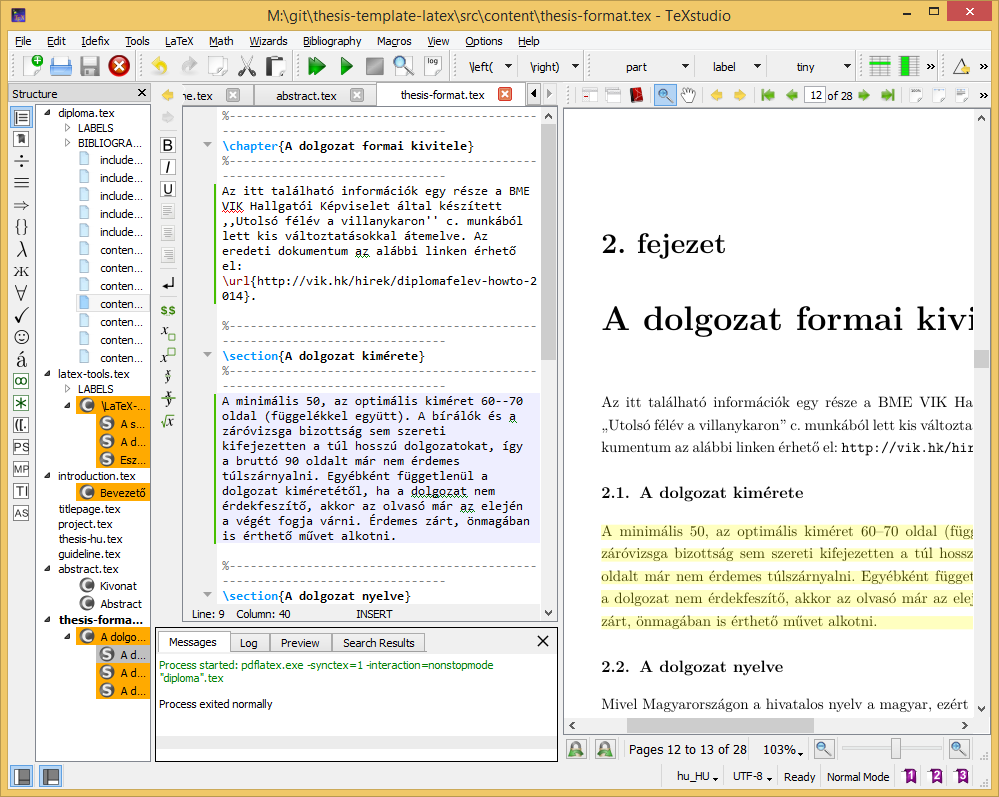
\includegraphics[width=67mm, keepaspectratio]{figures/TeXstudio.png}\hspace{1cm}
	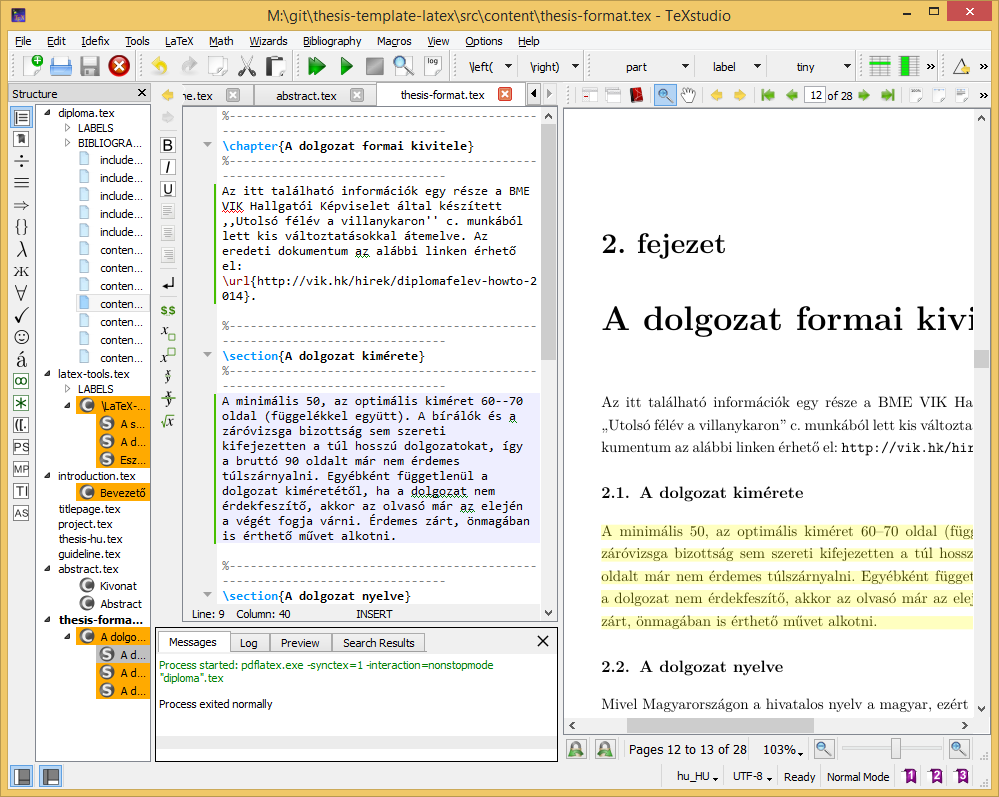
\includegraphics[width=67mm, keepaspectratio]{figures/TeXstudio.png}\\\vspace{5mm}
	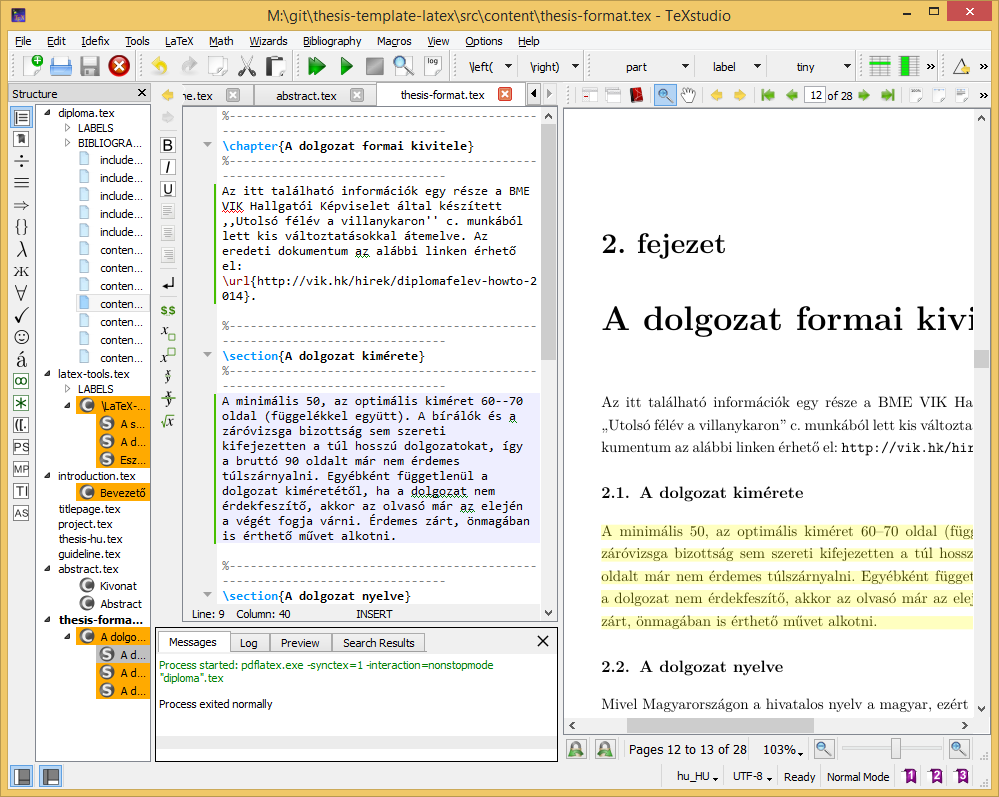
\includegraphics[width=67mm, keepaspectratio]{figures/TeXstudio.png}\hspace{1cm}
	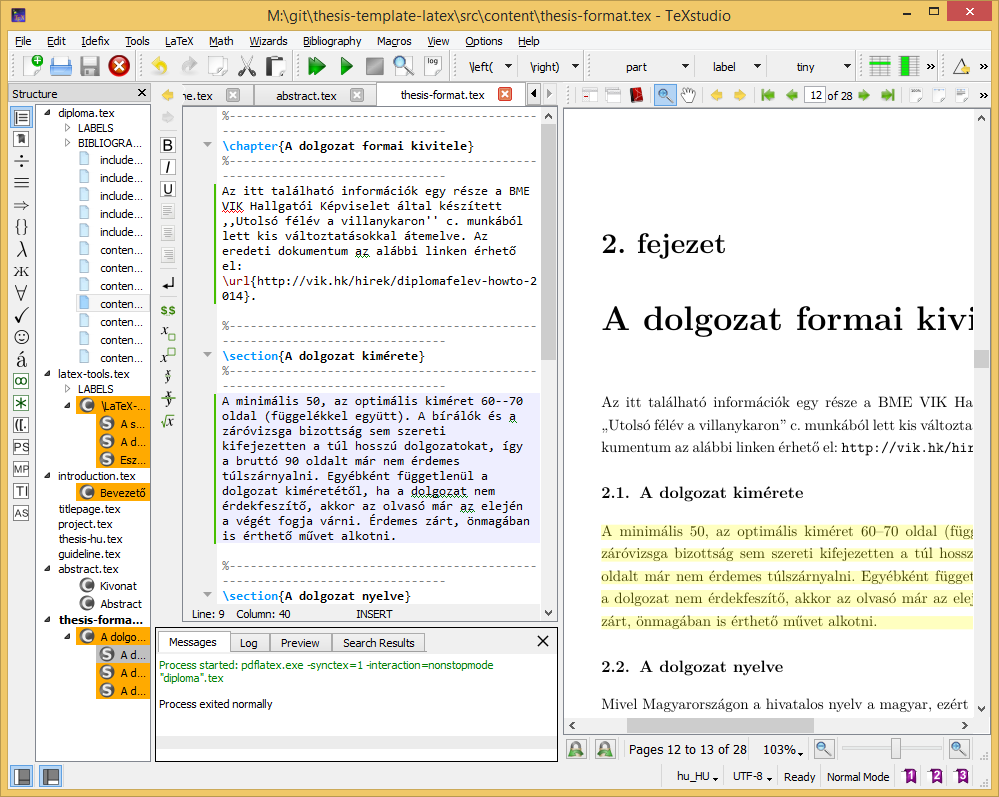
\includegraphics[width=67mm, keepaspectratio]{figures/TeXstudio.png}
	\caption{Több képfájl beillesztése esetén térközöket is érdemes használni.} 
	\label{fig:HVSpaces}
\end{figure}

A táblázatok használatára a \tabref{TabularExample}~táblázat mutat példát. A táblázat címkéje nem véletlenül került a táblázat fölé, ez a szokványos. A táblázatok formázásához hasznos tanácsokat találunk a \verb+booktabs+ csomag dokumentációjában.

\begin{table}[ht]
	\footnotesize
	\centering
	\caption{Az órajel-generátor chip órajel-kimenetei.} \label{tab:SysClocks}
	\begin{tabular}{ l c c }
		\toprule
		Órajel & Frekvencia & Cél pin \\
		\midrule
		CLKA & 100 MHz & FPGA CLK0\\
		CLKB & 48 MHz  & FPGA CLK1\\
		CLKC & 20 MHz  & Processzor\\
		CLKD & 25 MHz  & Ethernet chip \\
		CLKE & 72 MHz  & FPGA CLK2\\
		XBUF & 20 MHz  & FPGA CLK3\\
		\bottomrule
	\end{tabular}
	\label{tab:TabularExample}
\end{table}


%----------------------------------------------------------------------------
\section{Felsorolások és listák}
%----------------------------------------------------------------------------
Számozatlan felsorolásra mutat példát a jelenlegi bekezdés:
\begin{itemize}
	\item \emph{első bajusz:} ide lehetne írni az első elem kifejését,
	\item \emph{második bajusz:} ide lehetne írni a második elem kifejését,
	\item \emph{ez meg egy szakáll:} ide lehetne írni a harmadik elem kifejését.
\end{itemize}

Számozott felsorolást is készíthetünk az alábbi módon:
\begin{enumerate}
	\item \emph{első bajusz:} ide lehetne írni az első elem kifejését, és ez a kifejtés így néz ki, ha több sorosra sikeredik,
	\item \emph{második bajusz:} ide lehetne írni a második elem kifejését,
	\item \emph{ez meg egy szakáll:} ide lehetne írni a harmadik elem kifejését.
\end{enumerate}
A felsorolásokban sorok végén vessző, az utolsó sor végén pedig pont a szokásos írásjel. Ez alól kivételt képezhet, ha az egyes elemek több teljes mondatot tartalmaznak.

Listákban a dolgozat szövegétől elkülönítendő kódrészleteket, programsorokat, pszeudo-kódokat jeleníthetünk meg (\listref{Example}~lista). 
\begin{lstlisting}[caption=A fenti számozott felsorolás \LaTeX-forráskódja,label=listing:Example]
\begin{enumerate}
	\item \emph{els(*@ő@*) bajusz:} ide lehetne írni az els(*@ő@*) elem kifejését, 
	és ez a kifejtés így néz ki, ha több sorosra sikeredik,
	\item \emph{második bajusz:} ide lehetne írni a második elem kifejését,
	\item \emph{ez meg egy szakáll:} ide lehetne írni a harmadik elem kifejését.
\end{enumerate}
\end{lstlisting}
A lista keretét, háttérszínét, egész stílusát megválaszthatjuk. Ráadásul különféle programnyelveket és a nyelveken belül kulcsszavakat is definiálhatunk, ha szükséges. Erről bővebbet a \verb+listings+ csomag hivatalos leírásában találhatunk.

%----------------------------------------------------------------------------
\section{Képletek}
%----------------------------------------------------------------------------
Ha egy formula nem túlságosan hosszú, és nem akarjuk hivatkozni a szövegből, mint például a $e^{i\pi}+1=0$ képlet, \emph{szövegközi képletként} szokás leírni. Csak, hogy másik példát is lássunk, az $U_i=-d\Phi/dt$ Faraday-törvény a $\rot E=-\frac{dB}{dt}$ differenciális alakban adott Maxwell-egyenlet felületre vett integráljából vezethető le. Látható, hogy a \LaTeX-fordító a sorközöket betartja, így a szöveg szedése esztétikus marad szövegközi képletek használata esetén is.

Képletek esetén az általános konvenció, hogy a kisbetűk skalárt, a kis félkövér betűk ($\mathbf{v}$) oszlopvektort -- és ennek megfelelően $\mathbf{v}^T$ sorvektort -- a kapitális félkövér betűk ($\mathbf{V}$) mátrixot jelölnek. Ha ettől el szeretnénk térni, akkor az alkalmazni kívánt jelölésmódot célszerű külön alfejezetben definiálni. Ennek megfelelően, amennyiben $\mathbf{y}$ jelöli a mérések vektorát, $\mathbf{\vartheta}$ a paraméterek vektorát és $\hat{\mathbf{y}}=\mathbf{X}\vartheta$ a paraméterekben lineáris modellt, akkor a \emph{Least-Squares} értelemben optimális paraméterbecslő $\hat{\mathbf{\vartheta}}_{LS}=(\mathbf{X}^T\mathbf{X})^{-1}\mathbf{X}^T\mathbf{y}$ lesz.

Emellett kiemelt, sorszámozott képleteket is megadhatunk, ennél az \verb+equation+ és a \verb+eqnarray+ környezetek helyett a korszerűbb \verb+align+ környezet alkalmazását javasoljuk (több okból, különféle problémák elkerülése végett, amelyekre most nem térünk ki). Tehát
\begin{align}
\dot{\mathbf{x}}&=\mathbf{A}\mathbf{x}+\mathbf{B}\mathbf{u},\\
\mathbf{y}&=\mathbf{C}\mathbf{x},
\end{align}
ahol $\mathbf{x}$ az állapotvektor, $\mathbf{y}$ a mérések vektora és $\mathbf{A}$, $\mathbf{B}$ és $\mathbf{C}$ a rendszert leíró paramétermátrixok. Figyeljük meg, hogy a két egyenletben az egyenlőségjelek egymáshoz igazítva jelennek meg, mivel a mindkettőt az \& karakter előzi meg a kódban. Lehetőség van számozatlan kiemelt képlet használatára is, például
\begin{align}
\dot{\mathbf{x}}&=\mathbf{A}\mathbf{x}+\mathbf{B}\mathbf{u},\nonumber\\
\mathbf{y}&=\mathbf{C}\mathbf{x}\nonumber.
\end{align}
Mátrixok felírására az $\mathbf{A}\mathbf{x}=\mathbf{b}$ inhomogén lineáris egyenlet részletes kifejtésével mutatunk példát:
\begin{align}
\begin{bmatrix}
a_{11} & a_{12} & \dots & a_{1n}\\
a_{21} & a_{22} & \dots & a_{2n}\\
\vdots & \vdots & \ddots & \vdots\\
a_{m1} & a_{m2} & \dots & a_{mn}
\end{bmatrix}
\begin{pmatrix}x_1\\x_2\\\vdots\\x_n\end{pmatrix}=
\begin{pmatrix}b_1\\b_2\\\vdots\\b_m\end{pmatrix}.
\end{align}
A \verb+\frac+ utasítás hatékonyságát egy általános másodfokú tag átviteli függvényén keresztül mutatjuk be, azaz
\begin{align}
W(s)=\frac{A}{1+2T\xi s+s^2T^2}.
\end{align}
A matematikai mód minden szimbólumának és képességének a bemutatására természetesen itt nincs lehetőség, de gyors referenciaként hatékonyan használhatók a következő linkek:\\
\indent\url{http://www.artofproblemsolving.com/LaTeX/AoPS_L_GuideSym.php},\\
\indent\url{http://www.ctan.org/tex-archive/info/symbols/comprehensive/symbols-a4.pdf},\\
\indent\url{ftp://ftp.ams.org/pub/tex/doc/amsmath/short-math-guide.pdf}.\\
Ez pedig itt egy magyarázat, hogy miért érdemes \verb+align+ környezetet használni:\\
\indent\url{http://texblog.net/latex-archive/maths/eqnarray-align-environment/}.

%----------------------------------------------------------------------------
\section{Irodalmi hivatkozások}\label{sect:HowtoReference}
%----------------------------------------------------------------------------
Egy \LaTeX~dokumentumban az irodalmi hivatkozások definíciójának két módja van. Az egyik a \verb+\thebibliograhy+ környezet használata a dokumentum végén, az \verb+\end{document}+ lezárás előtt.
\begin{lstlisting}
\begin{thebibliography}{9}

\bibitem{Lamport94} Leslie Lamport, \emph{\LaTeX: A Document Preparation System}. 
Addison Wesley, Massachusetts, 2nd Edition, 1994.

\end{thebibliography}
\end{lstlisting}

Ezek után a dokumentumban a \verb+\cite{Lamport94}+ utasítással hivatkozhatunk a forrásra. A fenti megadás viszonylag kötetlen, a szerző maga formázza az irodalomjegyzéket (ami gyakran inkonzisztens eredményhez vezet). 

Egy sokkal professzionálisabb módszer a BiB\TeX~használata, ezért ez a sablon is ezt támogatja. Ebben az esetben egy külön szöveges adatbázisban definiáljuk a forrásmunkákat, és egy külön stílusfájl határozza meg az irodalomjegyzék kinézetét. Ez, összhangban azzal, hogy külön formátumkonvenció határozza meg a folyóirat-, a könyv-, a konferenciacikk- stb. hivatkozások kinézetét az irodalomjegyzékben (a sablon használata esetén ezzel nem is kell foglalkoznia a hallgatónak, de az eredményt célszerű ellenőrizni). A felhasznált hivatkozások adatbázisa egy \verb+.bib+ kiterjesztésű szöveges fájl, amelynek szerkezetét a \listref{Bibtex} kódrészlet demonstrálja. A forrásmunkák bevitelekor a sor végi vesszők külön figyelmet igényelnek, mert hiányuk a BiB\TeX-fordító hibaüzenetét eredményezi. A forrásmunkákat típus szerinti kulcsszó vezeti be (\verb+@book+ könyv, \verb+@inproceedings+ konferenciakiadványban megjelent cikk, \verb+@article+ folyóiratban megjelent cikk, \verb+@techreport+ valamelyik egyetem gondozásában megjelent műszaki tanulmány, \verb+@manual+ műszaki dokumentáció esetén stb.). Nemcsak a megjelenés stílusa, de a kötelezően megadandó mezők is típusról-típusra változnak. Egy jól használható referencia a \url{http://en.wikipedia.org/wiki/BibTeX} oldalon található.
\begin{lstlisting}[caption=Példa szöveges irodalomjegyzék-adatbázisra BiBTeX használata esetén.,label=listing:Bibtex]
@BOOK{Wettl04,
  author="Ferenc Wettl and Gyula Mayer and Péter Szabó",
  title="\LaTeX~kézikönyv",
  publisher="Panem Könyvkiadó",
  year=2004
}

@ARTICLE{Candy86,
  author ="James C. Candy",
  title  ="Decimation for Sigma Delta Modulation",
  journal="{IEEE} Trans.\ on Communications",
  volume =34,
  number =1,
  pages  ="72--76",
  month  =jan,
  year   =1986,
  note = {\doi{10.1109/TCOM.1986.1096432}},
}

@INPROCEEDINGS{Lee87,
  author =       "Wai L. Lee and Charles G. Sodini",
  title =        "A Topology for Higher Order Interpolative Coders",
  booktitle =    "Proc.\ of the IEEE International Symposium on Circuits and Systems",
  year =         1987,
  vol =          2,
  month =        may # "~4--7",
  address =      "Philadelphia, PA, USA",
  pages =        "459--462"
}

@PHDTHESIS{KissPhD,
  author =   "Peter Kiss",
  title =    "Adaptive Digital Compensation of Analog Circuit Imperfections for Cascaded Delta-Sigma Analog-to-Digital Converters",
  school =   "Technical University of Timi\c{s}oara, Romania",
  month =    apr,
  year =     2000
}

@MANUAL{Schreier00,
  author = "Richard Schreier",
  title  = "The Delta-Sigma Toolbox v5.2",
  organization = "Oregon State University",
  year   = 2000,
  month  = jan,
  note   ="\url{http://www.mathworks.com/matlabcentral/fileexchange/}"
}

@MISC{DipPortal,
	author = "{Budapesti Műszaki és Gazdaságtudományi Egyetem Villamosmérnöki és Informatikai Kar}",
	title = "Diplomaterv portál (2011. február 26.)",
	howpublished = "\url{http://diplomaterv.vik.bme.hu/}",
}

@incollection{Mkrtychev:1997,
	author={Mkrtychev, Alexey},
	title={Models for the logic of proofs},
	year={1997},
	editor={Adian, Sergei and Nerode, Anil},
	booktitle={Logical Foundations of Computer Science},
	series={Lecture Notes in Computer Science},
	volume={1234},
	pages={266-275},
	isbn={978-3-540-63045-6},
	doi={10.1007/3-540-63045-7_27},
	publisher={Springer Berlin Heidelberg},
	url={http://dx.doi.org/10.1007/3-540-63045-7_27},
}
\end{lstlisting}

A stílusfájl egy \verb+.sty+ kiterjesztésű fájl, de ezzel lényegében nem kell foglalkozni, mert vannak beépített stílusok, amelyek jól használhatók. Ez a sablon a BiB\TeX-et használja, a hozzá tartozó adatbázisfájl a \verb+mybib.bib+ fájl. Megfigyelhető, hogy az irodalomjegyzéket a dokumentum végére (a \verb+\end{document}+ utasítás elé) beillesztett \verb+\bibliography{mybib}+ utasítással hozhatjuk létre, a stílusát pedig ugyanitt a  \verb+\bibliographystyle{plain}+ utasítással adhatjuk meg. Ebben az esetben a \verb+plain+ előre definiált stílust használjuk (a sablonban is ezt állítottuk be). A \verb+plain+ stíluson kívül természetesen számtalan más előre definiált stílus is létezik. Mivel a \verb+.bib+ adatbázisban ezeket megadtuk, a BiB\TeX-fordító is meg tudja különböztetni a szerzőt a címtől és a kiadótól, és ez alapján automatikusan generálódik az irodalomjegyzék a stílusfájl által meghatározott stílusban.

Az egyes forrásmunkákra a szövegből továbbra is a \verb+\cite+ paranccsal tudunk hivatkozni, így a \listref{Bibtex}~kódrészlet esetén a hivatkozások rendre \verb+\cite{Wettl04}+, \verb+\cite{Candy86}+, \verb+\cite{Lee87}+, \verb+\cite{KissPhD}+, \verb+\cite{Schreirer00}+,
\verb+\cite{Mkrtychev:1997}+ és \verb+\cite{DipPortal}+. Az egyes forrásmunkák sorszáma az irodalomjegyzék bővítésekor változhat. Amennyiben az aktuális számhoz illeszkedő névelőt szeretnénk használni, használjuk az \verb+\acite{}+ parancsot.

Az irodalomjegyzékben alapértelmezésben csak azok a forrásmunkák jelennek meg, amelyekre található hivatkozás a szövegben, és ez így alapvetően helyes is, hiszen olyan forrásmunkákat nem illik az irodalomjegyzékbe írni, amelyekre nincs hivatkozás.

Mivel a fordítási folyamat során több lépésben oldódnak fel a szimbólumok, ezért gyakran többször is le kell fordítani a dokumentumot. Ilyenkor ez első 1-2 fordítás esetleg szimbólum-feloldásra vonatkozó figyelmeztető üzenettel zárul. Ha hibaüzenettel zárul bármelyik fordítás, akkor nincs értelme megismételni, hanem a hibát kell megkeresni. A \verb+.bib+ fájl megváltoztatáskor sokszor nincs hatása a változtatásnak azonnal, mivel nem mindig fut újra a BibTeX fordító. Ezért célszerű a változtatás után azt manuálisan is lefuttatni (TeXstudio esetén \verb+Tools/Bibliography+).

Hogy a szövegbe ágyazott hivatkozások kinézetét demonstráljuk, itt most sorban meghivatkozzuk a \cite{Wettl04}, \cite{Candy86}, \cite{Lee87}, \cite{KissPhD}, \cite{Schreier00} és \acite{Mkrtychev:1997}\footnote{Informatikai témában gyakran hivatkozunk cikkeket a Springer LNCS valamely kötetéből, ez a hivatkozás erre mutat egy helyes példát.} forrásmunkát, valamint \acite{DipPortal} weboldalt.

Megjegyzendő, hogy az ékezetes magyar betűket is tartalmazó \verb+.bib+ fájl az \verb+inputenc+ csomaggal betöltött \verb+latin2+ betűkészlet miatt fordítható. Ugyanez a \verb+.bib+ fájl hibaüzenettel fordul egy olyan dokumentumban, ami nem tartalmazza a \verb+\usepackage[latin2]{inputenc}+ sort. Speciális igény esetén az irodalmi adatbázis általánosabb érvényűvé tehető, ha az ékezetes betűket speciális latex karakterekkel helyettesítjük a \verb+.bib+ fájlban, pl. á helyett \verb+\'{a}+-t vagy ő helyett \verb+\H{o}+-t írunk. 

Oldaltörés következik (ld. forrás).
\newpage

%----------------------------------------------------------------------------
\section{A dolgozat szerkezete és a forrásfájlok}
%----------------------------------------------------------------------------
A diplomatervsablonban a TeX fájlok két alkönyvtárban helyezkednek el. Az \verb+include+ könyvtárban azok szerepelnek, amiket tipikusan nem kell szerkesztenünk, ezek a sablon részei (pl. címoldal). A \verb+content+ alkönyvtárban pedig a saját munkánkat helyezhetjük el. Itt érdemes az egyes fejezeteket külön TeX állományokba rakni.

A diplomatervsablon (a kari irányelvek szerint) az alábbi fő fejezetekből áll:
\begin{enumerate}
	\item 1 oldalas \emph{tájékoztató} a szakdolgozat/diplomaterv szerkezetéről (\verb+include/guideline.tex+), ami a végső dolgozatból törlendő,
	\item \emph{feladatkiírás} (\verb+include/project.tex+), a dolgozat nyomtatott verzójában ennek a helyére kerül a tanszék által kiadott, a tanszékvezető által aláírt feladatkiírás, a dolgozat elektronikus verziójába pedig a feladatkiírás egyáltalán ne kerüljön bele, azt külön tölti fel a tanszék a diplomaterv-honlapra,
	\item \emph{címoldal} (\verb+include/titlepage.tex+),
	\item \emph{tartalomjegyzék} (\verb+diploma.tex+),
	\item a diplomatervező \emph{nyilatkozat}a az önálló munkáról (\verb+include/declaration.tex+),
	\item 1-2 oldalas tartalmi \emph{összefoglaló} magyarul és angolul, illetve elkészíthető még további nyelveken is (\verb+content/abstract.tex+),
	\item \emph{bevezetés}: a feladat értelmezése, a tervezés célja, a feladat indokoltsága, a diplomaterv felépítésének rövid összefoglalása (\verb+content/introduction.tex+),
	\item sorszámmal ellátott \emph{fejezetek}: a feladatkiírás pontosítása és részletes elemzése, előzmények (irodalomkutatás, hasonló alkotások), az ezekből levonható következtetések, a tervezés részletes leírása, a döntési lehetőségek értékelése és a választott megoldások indoklása, a megtervezett műszaki alkotás értékelése, kritikai elemzése, továbbfejlesztési lehetőségek,
	\item esetleges \emph{köszönetnyilvánítás}ok (\verb+content/acknowledgement.tex+),
	\item részletes és pontos \emph{irodalomjegyzék} (ez a sablon esetében automatikusan generálódik a \verb+diploma.tex+ fájlban elhelyezett \verb+\bibliography+ utasítás hatására, a \sectref{HowtoReference}. fejezetben leírtak szerint),
	\item \emph{függelékek} (\verb+content/appendices.tex+).
\end{enumerate}

A sablonban a fejezetek a \verb+diploma.tex+ fájlba vannak beillesztve \verb+\include+ utasítások segítségével. Lehetőség van arra, hogy csak az éppen szerkesztés alatt álló \verb+.tex+ fájlt fordítsuk le, ezzel lerövidítve a fordítási folyamatot. Ezt a lehetőséget az alábbi kódrészlet biztosítja a \verb+diploma.tex+ fájlban.
\begin{lstlisting}
\includeonly{
	guideline,%
	project,%
	titlepage,%
	declaration,%
	abstract,%
	introduction,%
	chapter1,%
	chapter2,%
	chapter3,%
	acknowledgement,%
	appendices,%
}
\end{lstlisting}

Ha az alábbi kódrészletben az egyes sorokat a \verb+%+ szimbólummal kikommentezzük, akkor a megfelelő \verb+.tex+ fájl nem fordul le. Az oldalszámok és a tartalomjegyék természetesen csak akkor billennek helyre, ha a teljes dokumentumot lefordítjuk.

%----------------------------------------------------------------------------
\newpage
\section{Alapadatok megadása}
%----------------------------------------------------------------------------
A diplomaterv alapadatait (cím, szerző, konzulens, konzulens titulusa) a \verb+diploma.tex+ fájlban lehet megadni.

%----------------------------------------------------------------------------
\section{Új fejezet írása}
%----------------------------------------------------------------------------
A főfejezetek külön \verb+content+ könyvtárban foglalnak helyet. A sablonhoz 3 fejezet készült. További főfejezeteket úgy hozhatunk létre, ha új TeX fájlt készítünk a fejezet számára, és a \verb+diploma.tex+ fájlban, a \verb+\include+ és \verb+\includeonly+ utasítások argumentumába felvesszük az új \verb+.tex+ fájl nevét.


%----------------------------------------------------------------------------
\section{Definíciók, tételek, példák}
%----------------------------------------------------------------------------

\begin{definition}[Fluxuskondenzátor térerőssége]
Lorem ipsum dolor sit amet, consectetur adipiscing elit, sed do eiusmod tempor incididunt ut labore et dolore magna aliqua. Ut enim ad minim veniam, quis nostrud exercitation ullamco laboris nisi ut aliquip ex ea commodo consequat. 
\end{definition}

\begin{example}
Példa egy példára. Duis aute irure dolor in reprehenderit in voluptate velit esse cillum dolore eu fugiat nulla pariatur. Excepteur sint occaecat cupidatat non proident, sunt in culpa qui officia deserunt mollit anim id est laborum.
\end{example}

\begin{theorem}[Kovács tétele]
Duis aute irure dolor in reprehenderit in voluptate velit esse cillum dolore eu fugiat nulla pariatur. Excepteur sint occaecat cupidatat non proident, sunt in culpa qui officia deserunt mollit anim id est laborum.
\end{theorem}



% Acknowledgements
%~~~~~~~~~~~~~~~~~~~~~~~~~~~~~~~~~~~~~~~~~~~~~~~~~~~~~~~~~~~~~~~~~~~~~~~~~~~~~~~~~~~~~~
%----------------------------------------------------------------------------
\chapter*{\koszonetnyilvanitas}\addcontentsline{toc}{chapter}{\koszonetnyilvanitas}
%----------------------------------------------------------------------------

Munkám során lehetőségem nyílt megismerni egy új közösséget a Hyundai Technologies Center Kft. PE csoportjának tagjaként. Köszönettel tartozom Mariscsák Balázsnak és Futó Andrásnak a témába korábban befektetett munkájukért és tanácsaiékrt munkám során. Köszönettel tartozom továbbá magának c gének, hogy biztosították a munkámhoz szükséges eszközöket és időt.

Továbbá köszönettel tartozom még Dr. Varjasi Istvánnak, amiért BSc Önálló laboratórium óta segíti szakmai fejlődésem.


% List of Figures, Tables
%~~~~~~~~~~~~~~~~~~~~~~~~~~~~~~~~~~~~~~~~~~~~~~~~~~~~~~~~~~~~~~~~~~~~~~~~~~~~~~~~~~~~~~
\listoffigures\addcontentsline{toc}{chapter}{\abrakjegyzeke}
\listoftables\addcontentsline{toc}{chapter}{\tablazatokjegyzeke}


% Bibliography
%~~~~~~~~~~~~~~~~~~~~~~~~~~~~~~~~~~~~~~~~~~~~~~~~~~~~~~~~~~~~~~~~~~~~~~~~~~~~~~~~~~~~~~
\bibliography{bib/mybib}
\addcontentsline{toc}{chapter}{\irodalomjegyzek}


% Appendix
%~~~~~~~~~~~~~~~~~~~~~~~~~~~~~~~~~~~~~~~~~~~~~~~~~~~~~~~~~~~~~~~~~~~~~~~~~~~~~~~~~~~~~~
%----------------------------------------------------------------------------
\appendix
%----------------------------------------------------------------------------
\chapter*{\fuggelek}\addcontentsline{toc}{chapter}{\fuggelek}
\setcounter{chapter}{\appendixnumber}
%\setcounter{equation}{0} % a fofejezet-szamlalo az angol ABC 6. betuje (F) lesz
\numberwithin{equation}{section}
\numberwithin{figure}{section}
\numberwithin{lstlisting}{section}
%\numberwithin{tabular}{section}

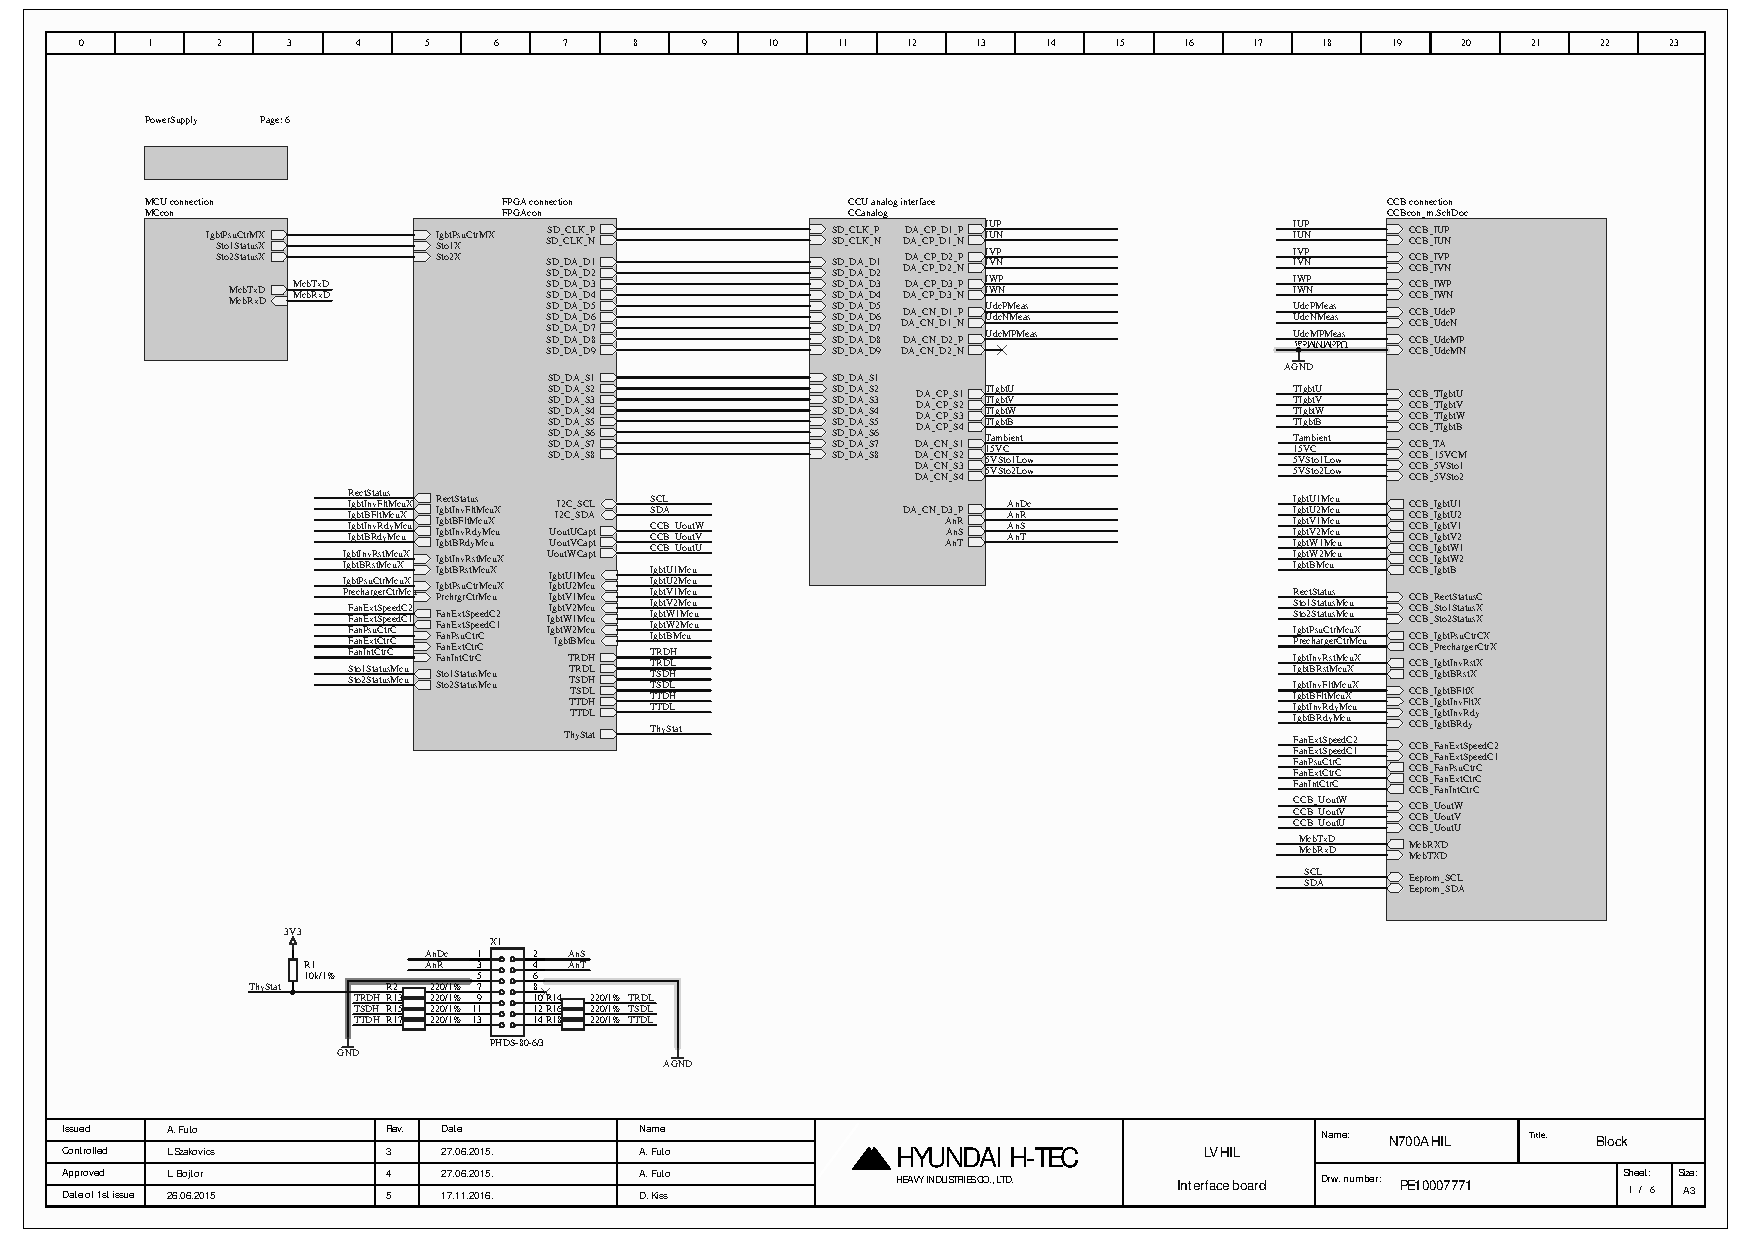
\includepdf[pages=-]{appendix/HIL.PDF}



%\label{page:last}
\end{document}
